\documentclass[a4paper]{article}

\usepackage[english]{babel}
\usepackage[utf8x]{inputenc}
\usepackage{amsmath,amsthm,enumitem}
\usepackage{graphicx}
\usepackage{lscape}
\usepackage{geometry}
\usepackage{color}
\usepackage{float}
\usepackage{listings}
\usepackage{amssymb}
\usepackage{verbatim}
\usepackage{algpseudocode} 
\usepackage{algorithm}  
\usepackage{algorithmicx}  
\usepackage{hyperref}
\usepackage{float}
\renewcommand{\baselinestretch}{1.5}
\usepackage{todonotes}
\geometry{left=2.5cm,right=2.5cm,top=2.5cm,bottom=2.5cm} 

\title{Note on Mathematics of Imaging}
\author{Haocheng Dai}
\date{}
\theoremstyle{definition}
\newtheorem{definition}{Definition}
% \newtheorem{definition}{Example}

\algnewcommand{\Inputs}[1]{%
  \State \textbf{Inputs:}\hspace*{\algorithmicindent}\parbox[t]{.8\linewidth}{\raggedright #1}
}

\theoremstyle{plain}
\newtheorem{theorem}{Theorem}
\newtheorem{lemma}{Lemma}
\newtheorem{remark}{Remark}
\newtheorem{corollary}{Corollary}
\newenvironment{example}[1][]{\refstepcounter{example}\par\medskip
   \noindent \textbf{Example~\theexample. #1} \rmfamily}{\medskip}
\newcounter{example}{Example}
      
\DeclareMathOperator*{\argmin}{arg\,min}
\DeclareMathOperator*{\argmax}{arg\,max}
\begin{document}
\maketitle

\section{Vector Space}
\begin{definition}
\fbox{\textbf{Inner product}}\cite{optimization} $\langle\cdot,\cdot\rangle:X\times X\rightarrow\mathbb{R}$ is a mapping that satisfies the following axioms:
\begin{enumerate}
    \item $\langle x,y\rangle=\langle y,x\rangle$
    \item $\langle x+y,z\rangle=\langle x,z\rangle+\langle y,z\rangle$
    \item $\langle\lambda x,y\rangle=\lambda\langle x,y\rangle$
    \item $\langle x,x\rangle\ge0$ and $\langle x,x\rangle=0$ if and only if $x=\theta$
\end{enumerate}
where $X$ is a vector space.
\end{definition}

\begin{example}
For $A,B\in \mathrm{GL}(n)$, the inner product $\langle A,B\rangle=\mathrm{Tr}(A^*B)$ and the associated norm $\|A\|_2=\mathrm{Tr}(A^*A)^{1/2}$.
\end{example}

\begin{definition}
\fbox{\textbf{Norm}} $\|\cdot\|:X\times X\rightarrow\mathbb{R}$ is a mapping that satisfies the following axioms:
\begin{enumerate}
    \item $\|x\|\ge0$ for all $x\in X$, $\|x\|=0$ if and only in $x=\theta$
    \item $\|x+y\|\le\|x\|+\|y\|$ for each $x,y\in X$ \Comment{Triangle inequality}
    \item $\|\alpha x\|=|\alpha|\cdot\|x\|$ for all scalars $\alpha$ and each $x\in X$
\end{enumerate}
where $X$ is a vector space.
\end{definition}

\begin{example}
The norm is clearly an abstraction of our usual concept of length. For continuous situation, the \textbf{supremum norm} $\|f\|_\infty$ is the supremum (lowest upper bound) of all elements of its domain evaluated in $f$. For discrete situation, the sup norm equals to the maximum of absolute values of its components, namely $\|f\|_\infty=\max |f_i|$.
\end{example}

\begin{remark}
If $f:\mathbb{R}^n\rightarrow\mathbb{R}, f(x)=\|x\|_p, p\ge1$, then $f$ is convex.
\end{remark}

\begin{figure}[H]\label{convex}
\centering
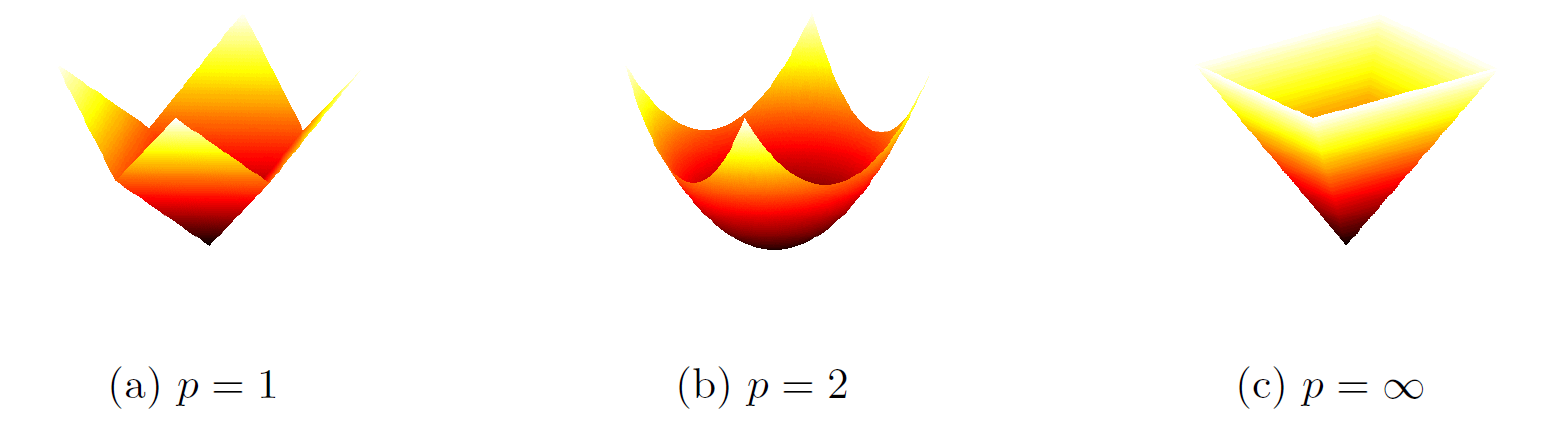
\includegraphics[scale=0.25]{figure/convex.png}
\caption{Image of 2D norm}
\end{figure}

\begin{definition}
\fbox{\textbf{$l_p$ space}} consists of all sequences of scalars $\{\xi_1,\xi_2,\cdots\}$ for which
\begin{equation*}
    \sum^\infty_{i=1}|\xi_i|^p<\infty
\end{equation*}
where $1\le p<\infty$.
\end{definition}
The norm of an element $x=\{\xi_i\}$ in $l_p$ is defined as 
\begin{equation*}
    \|x\|_p=\left(\sum^\infty_{i=1}|\xi_i|^p\right)^{1/p}
\end{equation*}

\begin{definition}
\fbox{\textbf{$L_p[a,b]$ space}} consists of all functions $f(u)$ for which
\begin{equation*}
    \int^b_a|f(u)|^pdu<\infty
\end{equation*}
where $1\le p<\infty$.
\end{definition}
The norm of an element $f(u)$ in $L_p$ is defined as 
\begin{equation*}
    \|f\|_p=\left(\int^b_a|f(u)|^pdu\right)^{1/p}
\end{equation*}
The $L^p$-functions are the functions for which this integral converges. For $p\not=2$, the space of $L^p$-functions is a Banach space which is not a Hilbert space.
% \todo{Always remember the \textbf{absolute value sign} in norm calculation.}
\begin{remark}
Always remember the \textbf{absolute value sign} in norm calculation.
\end{remark}

\begin{figure}[H]
\centering
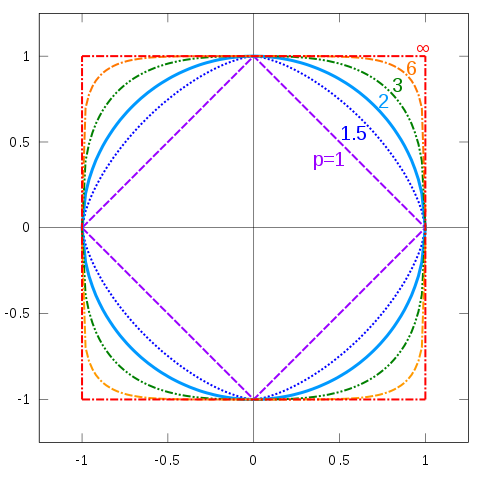
\includegraphics[scale=0.4]{figure/norm}
\caption{Visualization of $\|x\|_p=1$, which are the cross sections of Figure \ref{convex}.}
\end{figure}

\begin{definition}
\fbox{\textbf{Normed linear vector space}} is a vector space $X$ on which there is defined a real-valued function which maps each element $x$ in $X$ into a real number $\|x\|$.
\end{definition}

\begin{definition}
\fbox{\textbf{Pre-Hilbert space}} is a linear vector space $X$ together with an inner product defined on $X\times X$.
\end{definition}

\begin{definition}
\fbox{\textbf{Cauchy sequence}} is a sequence $\{x_n\}$ in a normed space such that $\|x_n-x_m\|\rightarrow0$ as $n,m\rightarrow\infty$.
\end{definition}
\begin{remark}
In a normed space, every convergent sequence is a Cauchy sequence, however, a Cauchy sequence may not be convergent.
\end{remark}

\begin{figure}[H]
\centering
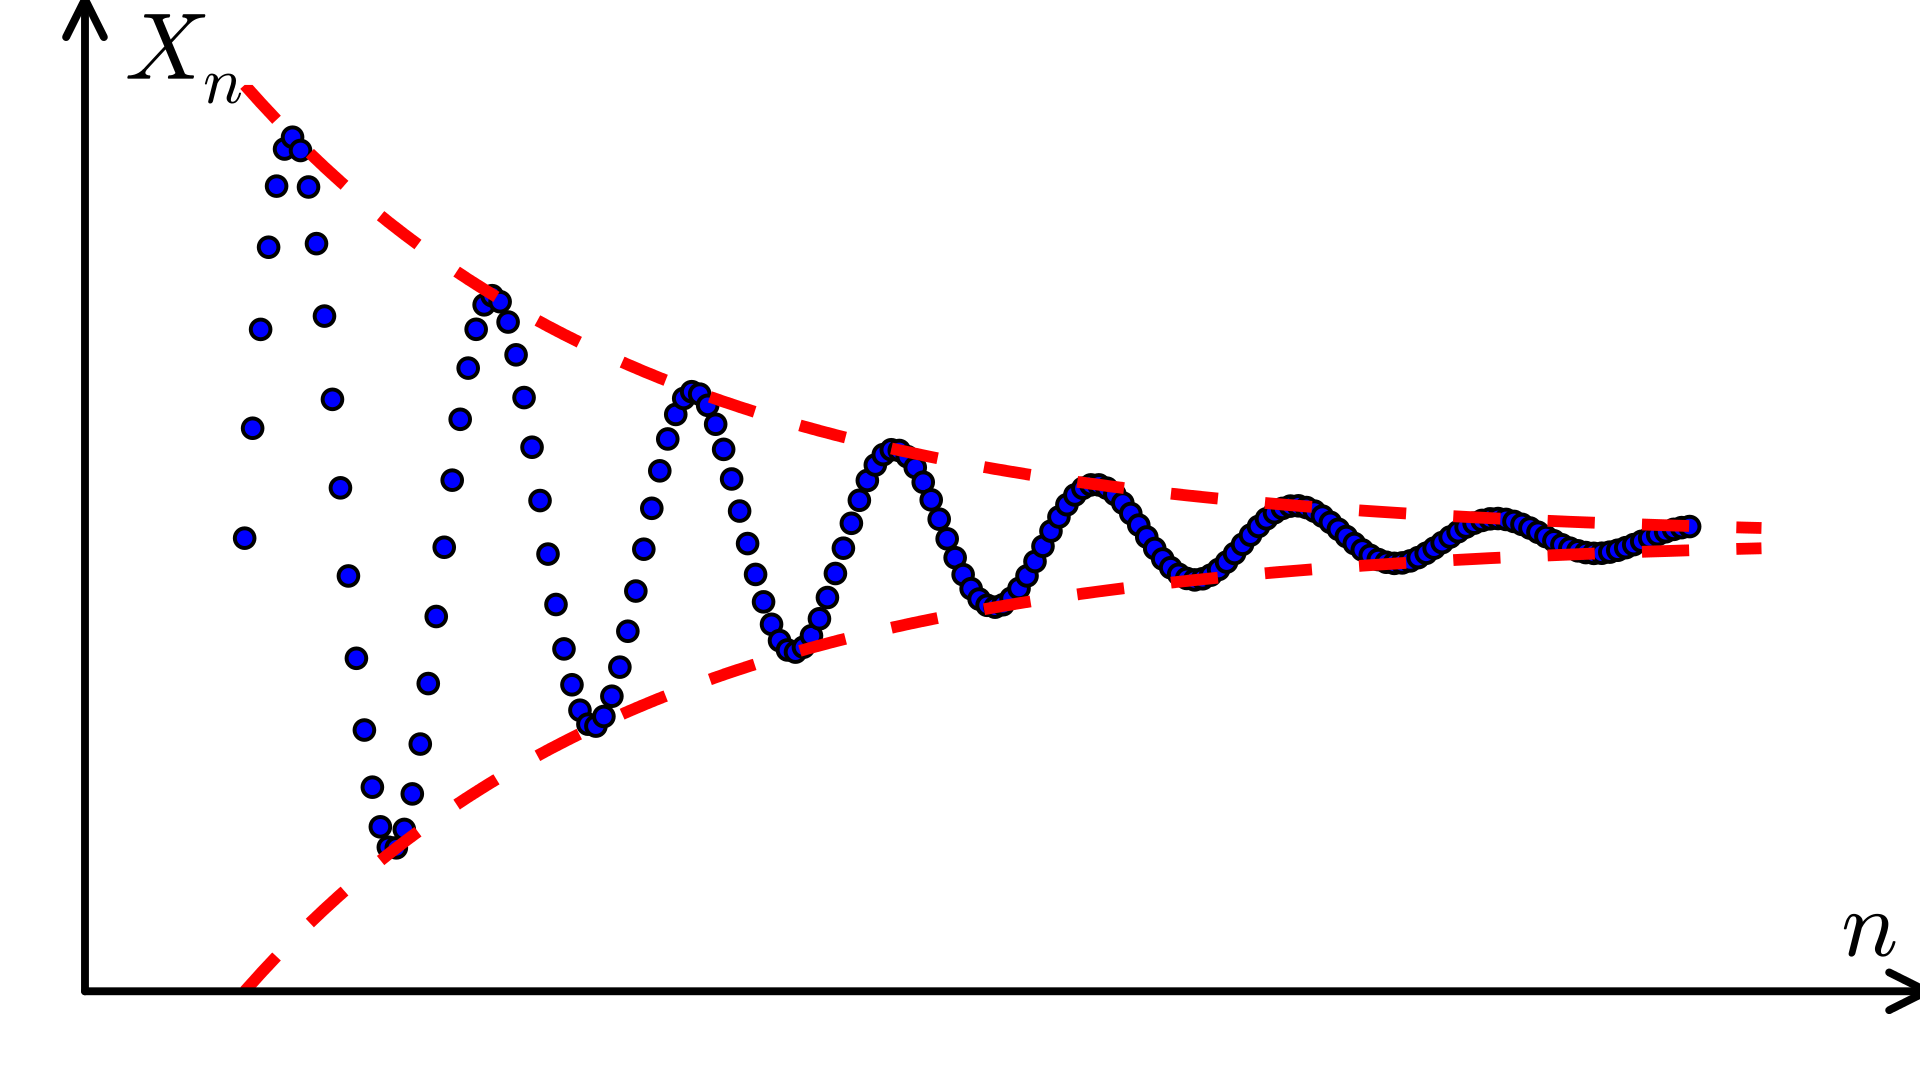
\includegraphics[scale=0.12]{figure/Cauchy_sequence}
\caption{Example of Cauchy sequence}
\end{figure}

\begin{definition}
A normed linear vector space $X$ is \fbox{\textbf{complete}} is every Cauchy sequence from $X$ has a limit in $X$. The limit is also a vector.
\end{definition}

\begin{definition}
\fbox{\textbf{Banach space}} is a complete normed linear vector space.
\end{definition}

\begin{definition}
\fbox{\textbf{Hilbert space}} is a complete pre-Hilbert space or a Banach space whose norm is defined by inner product.
\end{definition}

\begin{theorem}
\textbf{Holder Inequality}. If $p$ and $q$ are positive numbers $1\le p\le\infty, 1\le q\le\infty$, such that $1/p+1/q=1$ and if $x=\{\xi_1,\xi_2,\cdots\}\in l_p, y=\{\eta_1,\eta_2,\cdots\}\in l_q$, then
\begin{equation*}
    \sum^\infty_{i=1}|\xi_i\eta_i|\le\|x\|_p\cdot\|y\|_q
\end{equation*}
\end{theorem}
Equality holds if and only if $\left(\frac{|\xi_i|}{\|x\|_p}\right)^{1/q}=\left(\frac{|\eta_i|}{\|y\|_q}\right)^{1/p}$ for each $i$.
\begin{theorem}
\textbf{Cauchy-Schwarz Inequality}. If $p=2$ and $q=2$ and if $x=\{\xi_1,\xi_2,\cdots\}\in l_2, y=\{\eta_1,\eta_2,\cdots\}\in l_2$, then
\begin{equation*}
    \sum^\infty_{i=1}|\xi_i\eta_i|\le\|x\|_2\cdot\|y\|_2
\end{equation*}
\end{theorem}

\begin{theorem}
\textbf{Minkowski Inequality}. If $x$ and $y$ are in $l_p$, $1\le p\le\infty$, then
\begin{equation*}
    \|x+y\|_p\le\|x\|_p+\|y\|_p
\end{equation*}
\end{theorem}
Equality holds if and only if $k_1x=k_2y$ for some positive constants $k_1$ and $k_2$.

\begin{theorem}
\textbf{Divergence Theorem.} Letting $\varphi$ be a $C^1$ vector field, defined on $\Omega$, which is a region in the plane with boundary $\partial \Omega$, then
\begin{equation*}
    \int_\Omega\mathrm{div}\varphi dx=\int_{\partial\Omega}\langle\varphi,N\rangle dl
\end{equation*}
where $N$ is the outward normal to $\Omega$ and $\mathrm{div}(\varphi)=\mathrm{trace}(D\varphi)$.
\end{theorem}

\begin{definition}
\fbox{\textbf{Euler-Lagrange equation}} is defined as
\begin{equation*}
    \frac{\partial F}{\partial y}-\frac{\partial}{\partial x}\left(\frac{\partial F}{\partial y'}\right)=0.
\end{equation*}
which is used to find a $y=f(x)$ making this integral
\begin{equation*}
    L(y)=\int^{x_2}_{x_1}F(x,y,y')dx
\end{equation*}
stationary.
\end{definition}

\begin{example}
Suppose $A$ and $B$ are two points in a Euclidean space. We want to find the geodesic between $A$ and $B$.

\paragraph{Solution.} We would like to minimize 
\begin{align*}
    L&=\int^B_A1ds\text{, where } ds=\sqrt{(dx)^2+(dy)^2}=\sqrt{1+(y')^2}dx
\end{align*}
which can be written in another form
\begin{equation*}
    L=\int^B_A\sqrt{1+(y')^2}dx
\end{equation*}
We need to find a $y(x)$ which minimize $L$, where
\begin{equation*}
    F=\sqrt{1+(y')^2}
\end{equation*}
Substituting it into the Euler-Lagrange equation, we have
\begin{align*}
    \frac{\partial F}{\partial y}-\frac{d}{dx}\left(\frac{\partial F}{\partial y'}\right)&=0\\
    -\frac{d}{dx}\left(\frac{y'}{\sqrt{1+(y')^2}}\right)&=0\\
    \frac{y'}{\sqrt{1+(y')^2}}&=c\\
    (y')^2&=\frac{c^2}{1-c^2}\\
    y'&=c_1\\
    y&=c_1x+c_2
\end{align*}
\end{example}

\begin{theorem}
The property of a \textbf{Green's function} can be exploited to solve differential equations of the form
\begin{equation*}
    Lu(x)=f(x),
\end{equation*}
where $L$ and $f(x)$ are given. If the kernel of $L$ is non-trivial, then the Green's function is not unique.

A Green's function, $G(x,s)$ of a linear differential operator $L=L(x)$ at point $s$, is any solution of
\begin{equation*}
    LG(x,s)=\delta(s-x),
\end{equation*}
where $\delta$ is the Dirac delta function.

If such function $G$ can be found for the operator $L$, then we obtain
\begin{equation*}
    \int LG(x,s)f(s)ds=\int\delta(s-x)f(s)ds=f(x)
\end{equation*}

Because the operator $L=L(x)$ is linear and acts only on the variable $x$, one may take the operator $L$ outside of integration, yielding
\begin{equation*}
    L\left(\int G(x,s)f(s)ds\right)=f(x),
\end{equation*}
which means that 
\begin{equation*}
    u(x)=\int G(x,s)f(s)ds
\end{equation*}
is the solution to $Lu(x)=f(x)$.
\end{theorem}

\begin{definition}\cite{ucl}
\boxed{\textbf{Kernel}} $k:\mathcal{X}\times\mathcal{X}\rightarrow\mathbb{R}$ is a function, where $\mathcal{H}$ is a Hilbert space and $\mathcal{X}$ is a non-empty set, if there exists a function $\phi:\mathcal{X}\rightarrow\mathcal{H}$ such that for any $x,x'\in\mathcal{X}$, we have
\begin{align*}
    k(x,x')&:\mathcal{X}\times\mathcal{X}\rightarrow\mathbb{R}\\
    k(x,x')&=\langle \phi(x),\phi(x')\rangle_\mathcal{H}
\end{align*} 
\end{definition}

\begin{remark}
We imposed almost no conditions on $\mathcal{X}$: we don't even require there to be an inner product defined on the elements of $\mathcal{X}$. Defining inner product on $\mathcal{H}$ is enough. For example, let $x,x'$ represent two different books, we can't take an inner product between books, but we can take an inner product between the feature maps $\phi(x),\phi(x')$ corresponding to $x,x'$.
\end{remark}

\begin{remark}
Kernel gives a way to compute inner products in some feature space without even knowing what this space is and what is $\phi$. In most cases, we care more about the inner product than the feature mapping itself. We never need the coordinates of the data in the
feature space. One example is the Gaussian kernel $k(x,y)=\exp(−\gamma\|x−y\|^2)$. If we Taylor-expand this function, we'll see that it corresponds to an infinite-dimensional codomain of $\phi$.
\end{remark}

\begin{figure}[H]
\centering
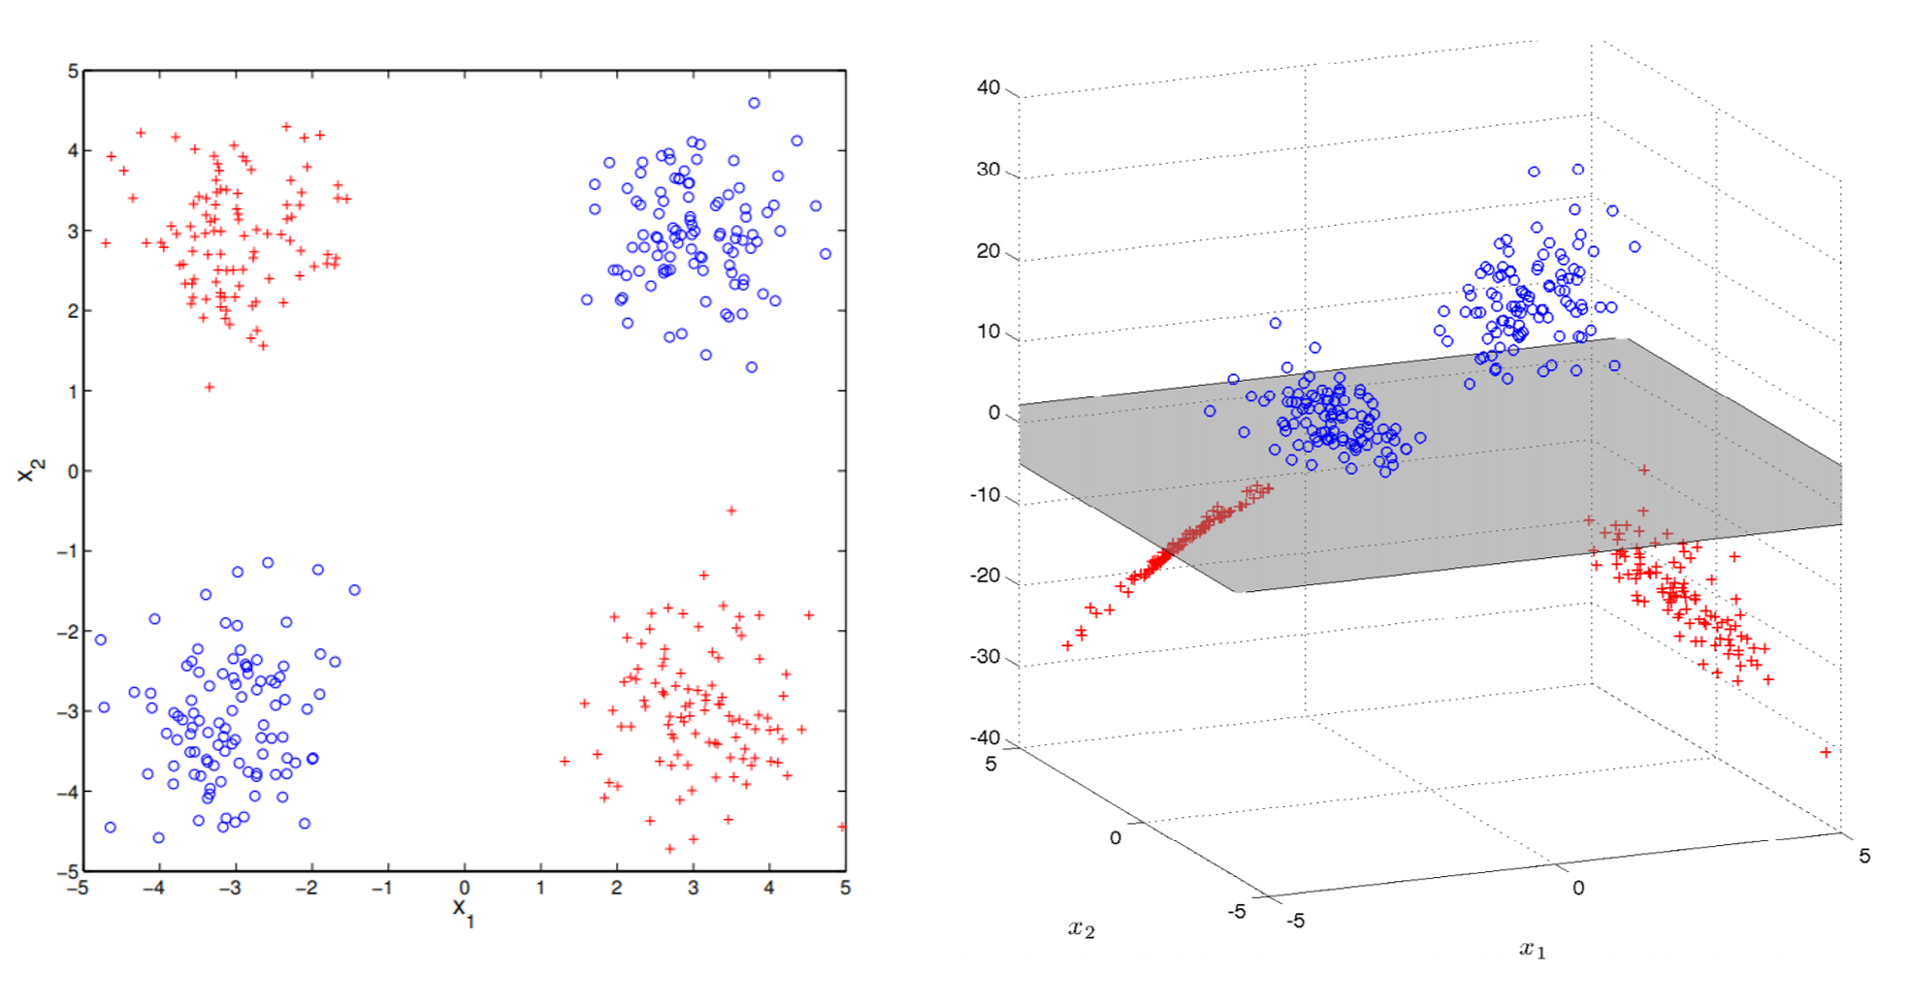
\includegraphics[scale=0.3]{figure/kernel.png}
\caption{$\phi(x)=[x_1,x_2,x_1x_2]^T$ example of kernel: on the left, the points are plotted in the original space; on the right, the points are plotted into a higher dimensional feature space by $\phi$.}
\end{figure}

\begin{definition}
\boxed{\textbf{Reproducing kernel}} $k:\mathcal{X}\times\mathcal{X}\rightarrow\mathbb{R}$ is a function, where $\mathcal{H}$ is a Hilbert space and $\mathcal{X}$ is a non-empty set, if $k$ satisfies
\begin{enumerate}
    \item $\forall x\in \mathcal{X},k(\cdot,x)\in\mathcal{H}$\Comment{Feature map of every point is in the feature space}
    \item $\forall x\in\mathcal{X},\forall f\in\mathcal{H},f(x)=\langle f,k(\cdot,x)\rangle_\mathcal{H}$\Comment{Reproducing property}
    \item $k(x,y)=\langle k(\cdot,x),k(\cdot,y)\rangle_\mathcal{H}=\langle \phi(x),\phi(y)\rangle_\mathcal{H}$
\end{enumerate}
\end{definition}

\begin{remark}
The feature map is not unique, only the kernel is. \textbf{RKHS functions} can be written as linear combination of feature maps $k(\cdot,x)$, which we can regard as ``basis function'':
\begin{align*}
    f(\cdot)&= \sum^m_{i=1}\alpha_i\phi_i(\cdot)=\sum^m_{i=1}\alpha_ik(\cdot,x_i)\\
    f(x)&=\langle f(\cdot),k(\cdot,x)\rangle_\mathcal{H}\\
    &=\left< \sum^m_{i=1}\alpha_ik(\cdot,x_i),k(\cdot,x)\right>_\mathcal{H}\\
    &= \sum^m_{i=1}\alpha_i\left<k(\cdot,x_i),k(\cdot,x)\right>_\mathcal{H}\\
    &= \sum^m_{i=1}\alpha_ik(x,x_i)
\end{align*}
\end{remark}

\begin{example}
We define a feature map $\phi:\mathbb{R}^2\rightarrow\mathbb{R}^3$
\begin{equation*}
    \phi(x)=[x_1,x_2,x_1x_2]^T
\end{equation*}
For the reproducing property, we define a RKHS function $f:\mathbb{R}^2\rightarrow\mathbb{R}$
\begin{align*}
    f(x)&=\sum^\infty_{l=1}f_l\phi_l(x) && \triangleright\text{Remark 3}\\
    &=ax_1+bx_2+cx_1x_2\\
    f(\cdot)&=[a, b, c]^T 
\end{align*}
where $f(\cdot)$ or $f$ stands for a function while $f(x)$ means the value of function $f$ at $x$.
With this, we can write
\begin{align*}
    f(x)&=f(\cdot)^T\phi(x)\\
    &=\langle f(\cdot),\phi(x)\rangle_\mathcal{H}
\end{align*}
The reproducing property tells us that the evaluation of $f$ at $x$ can be written as an inner product in feature space.
\end{example}

\begin{definition}
\boxed{\textbf{Primal-Dual method}}\\
Assume the primal problem as below:
\begin{align*}
    \text{maximize }&z(x)\\
    \text{subject to }&G(x)\le\theta && x\in\Omega
\end{align*}
which is equivalent to
\begin{align*}
    \text{minimize }&w(y)=\sup_{x\in\Omega}\{z(x)+\langle G(x),y\rangle\}\\
    \text{subject to }&y\ge\theta && x\in\Omega
\end{align*}
More specifically,
\paragraph{Primal}
\begin{align*}
    \text{maximize }z=\sum^n_{j=1}c_jx_j&\\
    \text{subject to }\sum^n_{j=1}a_{ij}x_j&\le b_i && (i=1,2,\cdots,m)\\
    x_j&\ge0 && (j=1,2,\cdots,n)
\end{align*}
\paragraph{Dual}
\begin{align*}
    \text{minimize }w=\sum^m_{i=1}b_iy_i&\\
    \text{subject to }\sum^m_{i=1}a_{ij}y_i&\ge c_j && (j=1,2,\cdots,n)\\
    y_i&\ge0 && (i=1,2,\cdots,m)
\end{align*}
\end{definition}

\begin{remark}
The difference between supremum (resp. infimum) and maximum (resp. minimum) is that for bounded, infinite sets, the maximum (resp. minimum) may not exist, but the supremum (resp. infimum) always does.
\end{remark}

\begin{figure}[H]
\centering
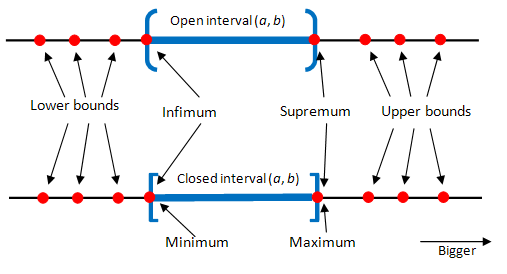
\includegraphics[scale=0.4]{figure/supinf.png}
\caption{Supremum and Infimum}
\end{figure}

\begin{example}
\paragraph{Primal}
\begin{align*}
\begin{array}{rrcrl}
    \text{max }&z=30x_1&+&100x_2&\\
    \text{s.t. }&x_1&+&x_2&\le7\\
    &4x_1&+&10x_2&\le40\\
    &x_1&&&\ge3\\
    &x_1&&&\ge0\\
    &&&x_2&\ge0 
\end{array}
\end{align*}
Multiply constraints $i$ by a factor $y_i$. Choose the sign of $y_i$ such that all inequalities are $\le$ after multiplication:
\begin{align*}
\begin{array}{rrcrll}
    \text{max }&z=30x_1&+&100x_2&&\\
    \text{s.t. }&x_1&+&x_2&\le7&\times y_1\\
    &4x_1&+&10x_2&\le40&\times y_2\\
    &x_1&&&\ge3&\times (-y_3)\\
    &x_1&&&\ge0&\times (-y_4)\\
    &&&x_2&\ge0& \times (-y_5)
\end{array}
\end{align*}
Add up all the obtained inequalities into a resultant inequality:
\begin{equation*}
    (y_1+4y_2-y_3-y_4)x_1+(y_1+10y_2-y_5)x_2\le7y_1+40y_2-3y_3
\end{equation*}
Make the coefficients of the resultant constraint match the objective function. Then, the right hand side of the resultant constraints is an upper bound of $z^*$:
\paragraph{Dual}
\begin{align*}
\begin{array}{ccccccccccccc}
    \text{min }&w=7y_1&+&40y_2&-&3y_3&\\
    \text{s.t. }&y_1&+&4y_2&-&y_3&-&y_4&&&&=&30\\
    &y_1&+&10y_2&&&&&&-&y_5&=&100\\
\end{array}
\end{align*}
\end{example}

\begin{remark}
Finding the max problem is equivalent to finding the min of the upper bound, that's why in the above example we should have the right sign of factor to make all inequalities are $\le$ after multiplication. Likewise, finding the min problem is equivalent to find the max of the lower bound.
\end{remark}

\begin{definition}
\boxed{\textbf{Thin plate splines}} are a spline-based technique for data interpolation and smoothing, which has the natural representation in terms of radial basis functions
\begin{equation*}
    f(x)=\sum^K_{i=1}w_i\varphi(\|x-c_i\|),
\end{equation*}
where $w_i$ is a set of mapping coefficient, $c_i$ is a set of control points and corresponding $\varphi$ for TPS is $\varphi(r)=r^2\log(r)$.

For 2D case, the energy function is defined as below
\begin{equation*}
    E_{\text{TPS},\text{smooth}}(f)=\sum^K_{i=1}\|y_i-f(x_i)\|^2+\lambda\int\int\left[\left(\frac{\partial^2 f}{\partial x^2_1}\right)^2+2\left(\frac{\partial^2f}{\partial x_1\partial x_2}\right)^2+\left(\frac{\partial^2f}{\partial x_2^2}\right)\right]dx_1dx_2
\end{equation*}
where the tuning parameter $\lambda$ is to control the rigidity of the deformation, balancing the aforementioned criterion with the measure of goodness of fit. If the interpolant pass through the data points exactly, then the first term of the energy function below should be zero. For this variational problem, it can be shown that there exists a unique minimizer $f$.
\end{definition}

\newpage
\section{Riemannian Geometry}
\begin{definition}
\boxed{\textbf{Isomorphism}}\cite{fletcher,hao,zhang} is a function between two structures of the same type that can be reversed by an inverse function.
\end{definition}

\begin{example}
In various areas of mathematics, isomorphisms have received specialized names, depending on the type of structure under consideration.
\begin{itemize}
    \item An \textbf{isometry} (Def.~\ref{def:isometry}) is an isomorphism of metric spaces.
    \item A \textbf{homeomorphism} (Def.~\ref{def:homeomorphism}) is an isomorphism of topological spaces.
    \item A \textbf{diffeomorphism} (Def.~\ref{def:diffeomorphism}) is an isomorphism of spaces equipped with a differential structure, typically differentiable manifolds.
\end{itemize}
\end{example}

\begin{definition}\label{def:homeomorphism}
\boxed{\textbf{Homeomorphism}} $f:M\rightarrow N$ is a bijective function between two topological spaces $M,N$, such that $f$ and $f^{-1}$ are both continuous function.
\end{definition}

\begin{definition}
\boxed{\textbf{Manifold}} is a Hausdorff space $M$ with a countable basis such that for each point $p\in M$ there is a neighborhood $u$ of $p$ that is homeomorphic to $\mathbb{R}^n$ for some integer $n$. In other words, locally, a manifold is like a Euclidean space.
\end{definition}

\begin{definition}\label{def:diffeomorphism}
\boxed{\textbf{Diffeomorphism}} $f:M\rightarrow N$ is a bijective function between two smooth manifolds $M, N$, such that $f$ and $f^{-1}$ are both smooth functions.
\end{definition}

\begin{remark}
For two manifolds $M$ and $N$, a smooth mapping $\phi:M\rightarrow N$ induces a linear mapping of the tangent spaces $\phi_*:T_pM\rightarrow T_{p\circ\phi}N$ called the \textbf{differential} of $\phi$.
\end{remark}

\begin{definition}
\boxed{\textbf{Tangent space}} $T_pM$ is a vector space attached to each point on a manifold $M$, which is equivalent to the Euclidean space. Intuitively, it's thought of as the linear space that best approximates $M$ in a neighborhood of point $p$. Vectors in this space are called tangent vectors.
\end{definition}

\begin{remark}
Tangent space means for each and every point $p$ in $\mathbb{R}^n$, we introduce a new coordinate system where all the vectors originated at $p$ will reside in.
\end{remark}

\begin{example}
The rotation group is presented as
\begin{equation*}
    \mathrm{SO}(3)=\{R\in \mathbb{R}^{3×3}|R^TR=I,|R|=1\}
\end{equation*}
In order to derive the form of elements in its Lie Algebra, $\mathfrak{so}(3)$, take a generic curve $R(t)$ through the identity in $\mathrm{SO}(3)$ with derivative $X\in\mathfrak{so}(3)$ at $t=0$ and consider the derivative of the constraint at $t=0$. The product rule yields
\begin{equation*}
    \frac{d}{dt}\bigg\rvert_{t=0}R(t)^TR(t)=X^T+X=0
\end{equation*}
This implies that any element of $\mathfrak{so}(3)$ is a \textbf{skew-symmetric matrix}.
\end{example}

\begin{remark}
The \textbf{cross product} of vector $a$ and $b$ can be written as below
\begin{equation*}
    a\times b=[a]_\times b=
    \begin{pmatrix}
        0 & -a_3 & a_2\\
        a_3 & 0 & -a_1\\
        -a_2 & a_1 & 0
    \end{pmatrix}\cdot
    \begin{pmatrix}
        b_1\\
        b_2\\
        b_3
    \end{pmatrix},
\end{equation*}
namely a skew-symmetric matrix times the vector $b$.
\end{remark}

\begin{example}
The group of symmetric positive definite matrices is presented as
\begin{equation*}
    \mathrm{SPD}(n)=\{X\in \mathbb{R}^{n×n}|X=X^T,X>0\}.
\end{equation*}
The tangent space $T_A\mathrm{SPD}(n)$ at $A$, is the space of symmetric matrices \cite{yger}.
\end{example}

\begin{definition}
\boxed{\textbf{Tangent bundle}} $TM$ consists of the tangent space $T_pM$ at all points $p$ in $M$. 
\begin{equation*}
     TM=\{(p,v)|p \in M,v \in T_pM\} 
\end{equation*}
Since a tangent space $T_pM$ is the set of all tangent vectors to $M$ at $p$, the tangent bundle is the collection of all tangent vectors, along with the information of the point to which they are tangent.
\end{definition}

\begin{definition}
\boxed{\textbf{Hessian matrix}} of a differentiable, multivariable function $f:\mathbb{R}^n\rightarrow\mathbb{R}$ at $p$ is defined by
\begin{equation*}
    Hf_p=
    \begin{pmatrix}
    \partial^2_1f_p & \partial_1\partial_2f_p & \cdots & \partial_1\partial_nf_p\\
    \partial_2\partial_1f_p & \partial^2_2f_p & \cdots & \partial_2\partial_nf_p\\
    \vdots & \vdots & \ddots & \vdots\\
    \partial_n\partial_1f_p & \partial_n\partial_2f_p & \cdots & \partial^2_nf_p
    \end{pmatrix}.
\end{equation*}
\end{definition}

\begin{remark}
    If multivariable function $f:\mathbb{R}^n\rightarrow\mathbb{R}, \nabla f(x)=0, Hf(x)$ is positive (resp. negative) definite, then $x$ is the isolated local minimum (resp. maximum).
\end{remark}

\begin{remark}
Relationship between convexity and positive-definiteness:
\begin{align*}
    f \text{ is convex}&\Leftrightarrow \forall p, Hf_p\text{ is positive semi–definite}\\
    f \text{ is strictly convex}&\Leftrightarrow \forall p, Hf_p\text{ is positive definite}
\end{align*}
\end{remark}

\begin{definition}
\boxed{\textbf{Laplacian}} of a differentiable, multivariable function $f:\mathbb{R}^n\rightarrow\mathbb{R}$ at $p$ is defined by
\begin{equation*}
    \Delta f_p=\operatorname{tr}(Hf_p)=\sum^n_{i=1}\partial^2_if_p.
\end{equation*}
\end{definition}

\begin{definition}
\boxed{\textbf{Jacobian matrix}}(differential) of a differentiable, vector-valued function $f:\mathbb{R}^n\rightarrow\mathbb{R}^m$ at $p$ is defined by \cite{stanford}
\begin{equation*}
    Df_p=
    \begin{pmatrix}
    \partial_1f^1_p & \partial_2f^1_p & \cdots & \partial_nf^1_p\\
    \partial_1f^2_p & \partial_2f^2_p & \cdots & \partial_nf^2_p\\
    \vdots & \vdots & \ddots & \vdots\\
    \partial_1f^m_p & \partial_2f^m_p & \cdots & \partial_nf^m_p
    \end{pmatrix},
\end{equation*}
where
\begin{equation*}
    f(x^1,\cdots,x^n)=\begin{pmatrix}
    f^1(x^1,\cdots,x^n)\\
    \vdots\\
    f^m(x^1,\cdots,x^n)
    \end{pmatrix}.
\end{equation*}
\end{definition}

\begin{definition}
\boxed{\textbf{Divergence}} of a differentiable, vector-valued function $f:\mathbb{R}^n\rightarrow\mathbb{R}^m$ at $p$ is defined by
\begin{equation*}
    \nabla\cdot f_p=\operatorname{tr}(Df_p)=\sum^n_{i=1}\partial_if^i_p.
\end{equation*}
\end{definition}

\begin{remark}
The Jacobian of $\nabla f$, where $f:\mathbb{R}^n\rightarrow\mathbb{R}$, is the Laplacian of $f$.
\end{remark}

\begin{remark}
As we all know, a matrix can be thought of as a linear transformation. Here as well, we can think of $Df_p$ as a linear function $Df_p:T_p\mathbb{R}^n\rightarrow T_p\mathbb{R}^m$. In other words, $Df_p$ maps a vector in the tangent space at the source point $p$ to a vector in the tangent space at the target point $f(p)$. More formally, we have
\begin{equation*}
    \frac{d}{dt}f(\gamma(t))\rvert_{t=0}=Df_p\cdot v_p\text{ ,where } v\in T_p\mathbb{R}^n
\end{equation*}
\end{remark}

\begin{figure}[H]
   \centering
   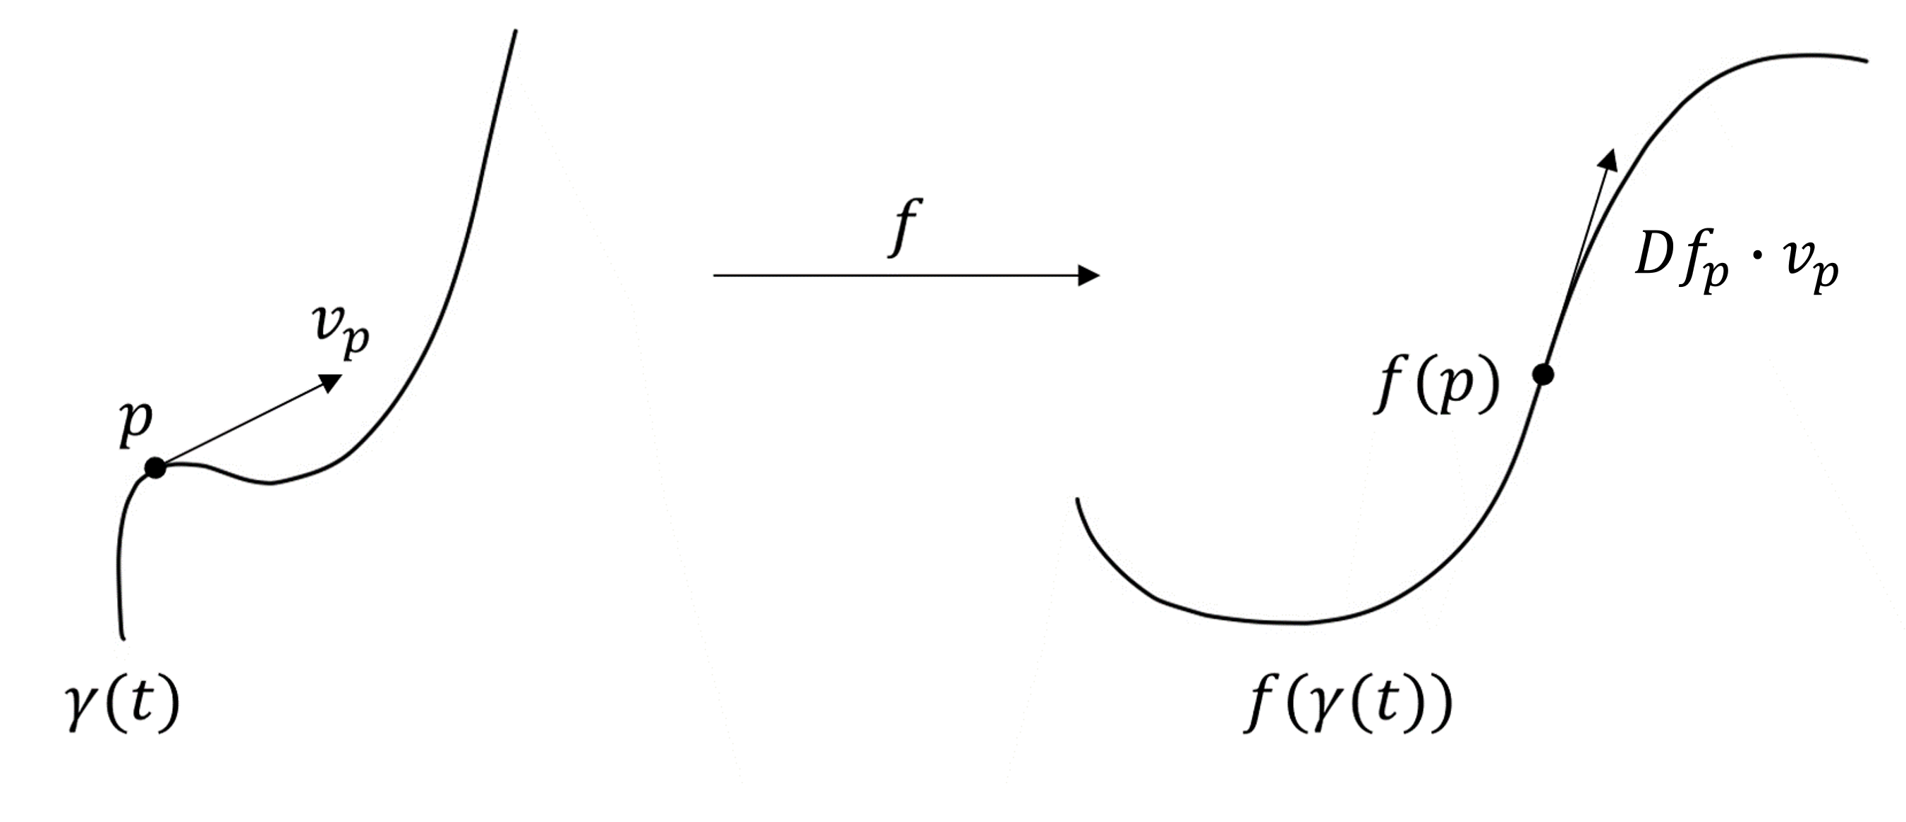
\includegraphics[scale=0.3]{figure/jacobian.png}
   \caption{Jacobian}
\end{figure}

\begin{remark}
The \textbf{determinant} of Jacobian at a given point gives important information about the behavior of $f$ near that point. 
\begin{itemize}
    \item If the Jacobian determinant at $p$ is non-zero, then $f$ is invertible near a point $p\in\mathbb{R}^n$.
    \item If the Jacobian determinant at $p$ is positive (resp. negative), then $f$ preserves (resp. reverses) orientation near $p$.
    \item The absolute value of the Jacobian determinant at $p$ gives us the factor by which the function $f$ expands or shrinks volumes near $p$.
\end{itemize}
\end{remark}

\begin{example}
For vector field $f:\mathbb{R}^2\rightarrow\mathbb{R}^2$:
\begin{equation*}
    Df=
    \begin{pmatrix}
    \frac{\partial f^1}{\partial x^1} & \frac{\partial f^1}{\partial x^2}\\
    \frac{\partial f^2}{\partial x^1} & \frac{\partial f^2}{\partial x^2}\\
    \end{pmatrix}
\end{equation*}
\end{example}

\begin{definition}
\boxed{\textbf{Vector field}} is a function on a manifold $M$ that smoothly assigns to each point $p\in M$ a tangent vector $v\in T_pM$.
\end{definition}

\begin{figure}[H]
   \centering
   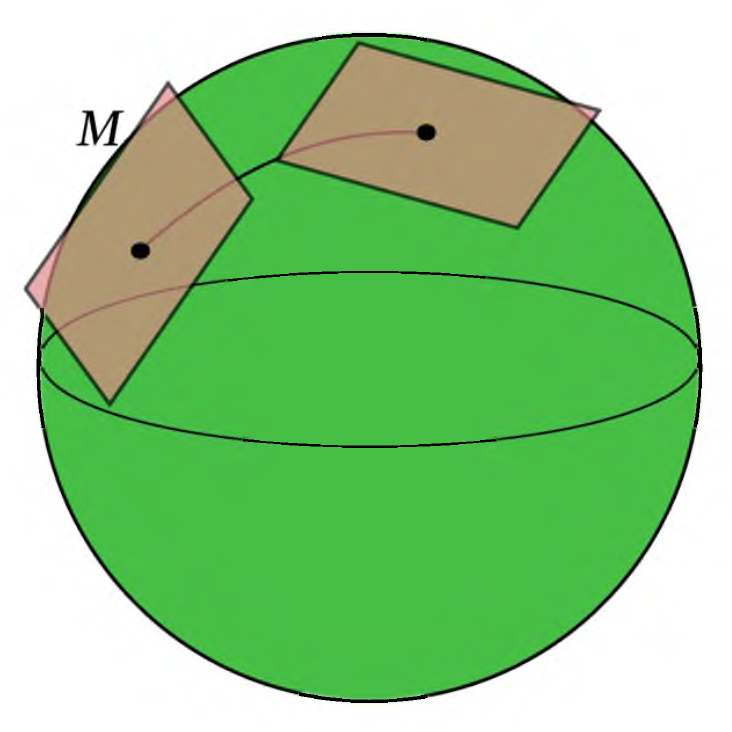
\includegraphics[scale=0.3]{figure/tangentspace.png}
   \caption{Tangent Space}
\end{figure}

\begin{definition}
\boxed{\textbf{Riemannian metric}} on a differential manifold $M$ is a smooth function that assigns to each point $p$ of $M$ an inner product $\langle\cdot,\cdot\rangle$ on the tangent space $T_pM$.
\end{definition}

\begin{definition}
\boxed{\textbf{Metric tensor}}\cite{metric} is a function which tells how to compute the distance between any two points in a given space.
\end{definition}

\begin{example}
Typically, we calculate the arc length as below
\begin{align*}
    \text{arc length}&=\int\|\dot\gamma(t)\|dt
\end{align*}

\begin{figure}[H]
   \centering
   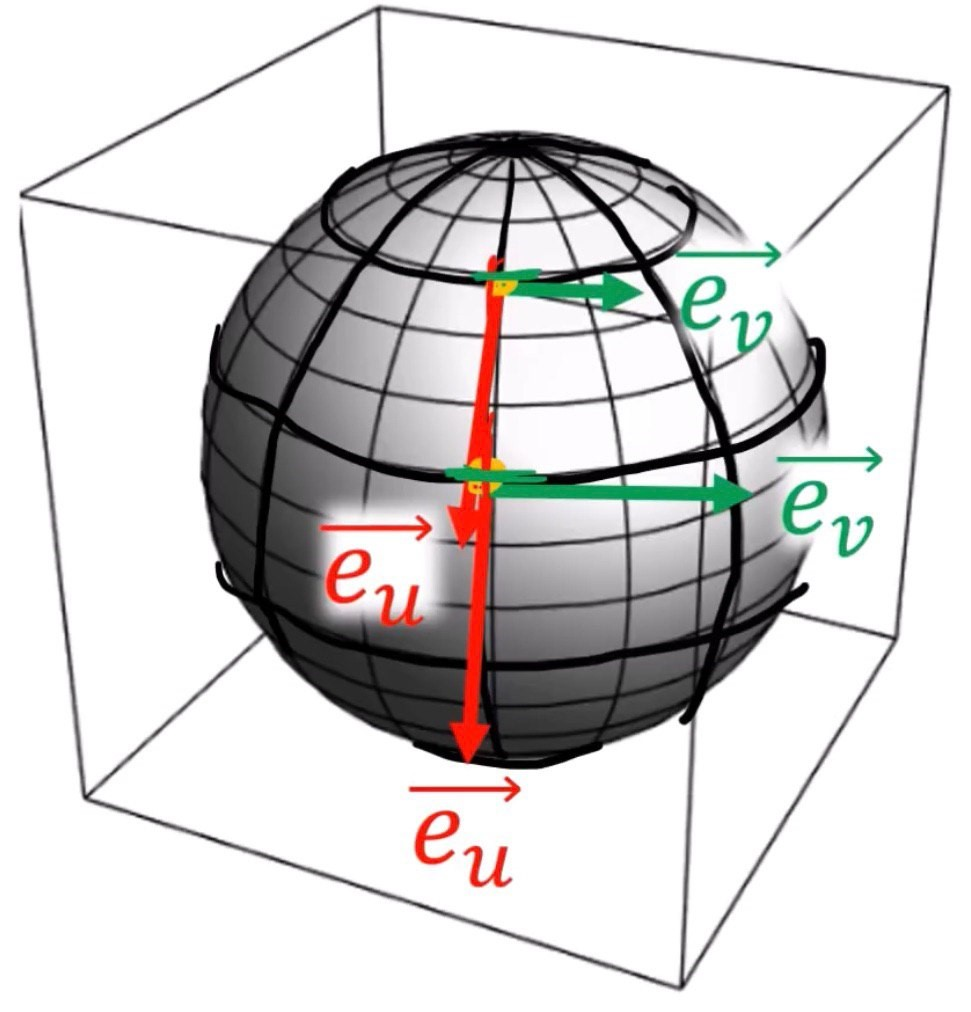
\includegraphics[scale=0.15]{figure/basevector.jpg}
   \caption{Base vectors on tangent space}
\end{figure}

By introducing the position vector, and expand it intrinsically, we can have
\begin{align*}
    \left\|\frac{d\vec R}{d\lambda}\right\|^2&=\frac{d\vec R}{d\lambda}\cdot\frac{d\vec R}{d\lambda}\\
    &=\left(\frac{d\vec R}{du}\cdot\frac{du}{d\lambda}+\frac{d\vec R}{dv}\cdot\frac{dv}{d\lambda}\right)\cdot\left(\frac{d\vec R}{du}\cdot\frac{du}{d\lambda}+\frac{d\vec R}{dv}\cdot\frac{dv}{d\lambda}\right)\\
    &=\left(\frac{du}{d\lambda}\right)^2\left(\frac{d\vec R}{du}\cdot\frac{d\vec R}{du}\right)+\frac{du}{d\lambda}\cdot\frac{dv}{d\lambda}\left(\frac{d\vec R}{du}\cdot\frac{d\vec R}{dv}\right)\\
    &+\frac{dv}{d\lambda}\cdot\frac{du}{d\lambda}\left(\frac{d\vec R}{dv}\cdot\frac{d\vec R}{du}\right)+\left(\frac{dv}{d\lambda}\right)^2\left(\frac{d\vec R}{dv}\cdot\frac{d\vec R}{dv}\right)\\
    &=\begin{pmatrix}
        \frac{du}{d\lambda}&\frac{dv}{d\lambda}
    \end{pmatrix}
    \underbrace{\begin{pmatrix}
        \frac{d\vec R}{du}\cdot\frac{d\vec R}{du} & \frac{d\vec R}{du}\cdot\frac{d\vec R}{dv}\\
        \frac{d\vec R}{dv}\cdot\frac{d\vec R}{du} & \frac{d\vec R}{dv}\cdot\frac{d\vec R}{dv}
    \end{pmatrix}}_{\text{metric tensor}}
    \begin{pmatrix}
        \frac{du}{d\lambda}\\
        \frac{dv}{d\lambda}
    \end{pmatrix}&&\text{$\triangleright\vec e_u=\frac{d\vec R}{du},\vec e_v=\frac{d\vec R}{dv}$}\\
    &=\begin{pmatrix}
        \frac{du}{d\lambda}&\frac{dv}{d\lambda}
    \end{pmatrix}
    \underbrace{\begin{pmatrix}
        \vec e_u\cdot\vec e_u & \vec e_u\cdot\vec e_v\\
        \vec e_v\cdot\vec e_u & \vec e_v\cdot\vec e_v
    \end{pmatrix}}_{\text{metric tensor}}
    \begin{pmatrix}
        \frac{du}{d\lambda}\\
        \frac{dv}{d\lambda}
    \end{pmatrix}
\end{align*}
\begin{remark}
Actually, without seeing the manifold extrinsically, it's hard to derive the metric, as we don't know the position vector. Provided that the metric is already given, so can we calculate what we want intrinsically.
\end{remark}

The parametric equation of a sphere is shown as below:
\begin{align*}
    \vec R&=[X,Y,Z]^T\\
    \text{where }X&=\cos(v)\sin(u)=\cos(\lambda)\sin(\lambda)\\
    Y&=\sin(v)\sin(u)=\sin(\lambda)\sin(\lambda)\\
    Z&=\cos(u)=\cos(\lambda)\\
    \text{when }u&=\lambda,v=\lambda.
\end{align*}

After expanding the base vectors extrinsically, we can have the base vectors expressed as below:
\begin{align*}
    \vec e_u=\frac{d\vec R}{du}&=\frac{\partial\vec R}{\partial X}\frac{\partial X}{\partial u}+\frac{\partial\vec R}{\partial Y}\frac{\partial Y}{\partial u}+\frac{\partial\vec R}{\partial Z}\frac{\partial Z}{\partial u}\\
    &=\cos(v)\cos(u)\frac{\partial\vec R}{\partial X}+\sin(v)\cos(u)\frac{\partial\vec R}{\partial Y}-\sin(u)\frac{\partial\vec R}{\partial Z}\\
    &=\cos(v)\cos(u)\vec e_X+\sin(v)\cos(u)\vec e_Y-\sin(u)\vec e_Z\\
    \vec e_v=\frac{d\vec R}{dv}&=\frac{\partial\vec R}{\partial X}\frac{\partial X}{\partial u}+\frac{\partial\vec R}{\partial Y}\frac{\partial Y}{\partial u}+\frac{\partial\vec R}{\partial Z}\frac{\partial Z}{\partial u}\\
    &=-\sin(v)\sin(u)\frac{\partial\vec R}{\partial X}+\cos(v)\sin(u)\frac{\partial\vec R}{\partial Y}\\
    &=-\sin(v)\sin(u)\vec e_X+\cos(v)\sin(u)\vec e_Y
\end{align*}

Since $\vec e_X,\vec e_Y,\vec e_Z$ are perpendicular to each other, so the metric tensor is yielded as below:
\begin{align*}
    \begin{pmatrix}
        \vec e_u\cdot\vec e_u & \vec e_u\cdot\vec e_v\\
        \vec e_v\cdot\vec e_u & \vec e_v\cdot\vec e_v
    \end{pmatrix}
    =\begin{pmatrix}
        1&0\\
        0&\sin^2(u)
    \end{pmatrix}
\end{align*}

Substituting the metric tensor back into the expression of norm of velocity, we get
\begin{align*}
    \left\|\frac{d\vec R}{d\lambda}\right\|^2&=
    \begin{pmatrix}
        \frac{du}{d\lambda}&\frac{dv}{d\lambda}
    \end{pmatrix}
    \begin{pmatrix}
        1&0\\
        0&\sin^2(u)
    \end{pmatrix}
    \begin{pmatrix}
        \frac{du}{d\lambda}\\
        \frac{dv}{d\lambda}
    \end{pmatrix}\\
    &=\left(\frac{du}{d\lambda}\right)^2+\sin^2(u)\left(\frac{dv}{d\lambda}\right)^2
\end{align*}

\begin{itemize}
    \item For $u=\frac{\pi}{4},v=\lambda$
    \begin{align*}
         \left\|\frac{d\vec R}{d\lambda}\right\|^2&=\left(\frac{du}{d\lambda}\right)^2+\sin^2(u)\left(\frac{dv}{d\lambda}\right)^2\\
         &=0^2+\sin^2\left(\frac{\pi}{4}\right)\cdot1^2=\frac{1}{2}
    \end{align*}
    The functional of arc length is
    \begin{equation*}
        \text{arc length}=\int\left\|\frac{d\vec R}{d\lambda}\right\|dt=\int\frac{\sqrt{2}}{2}dt=\frac{\sqrt{2}}{2}t
    \end{equation*}
    \begin{figure}[H]
        \centering
        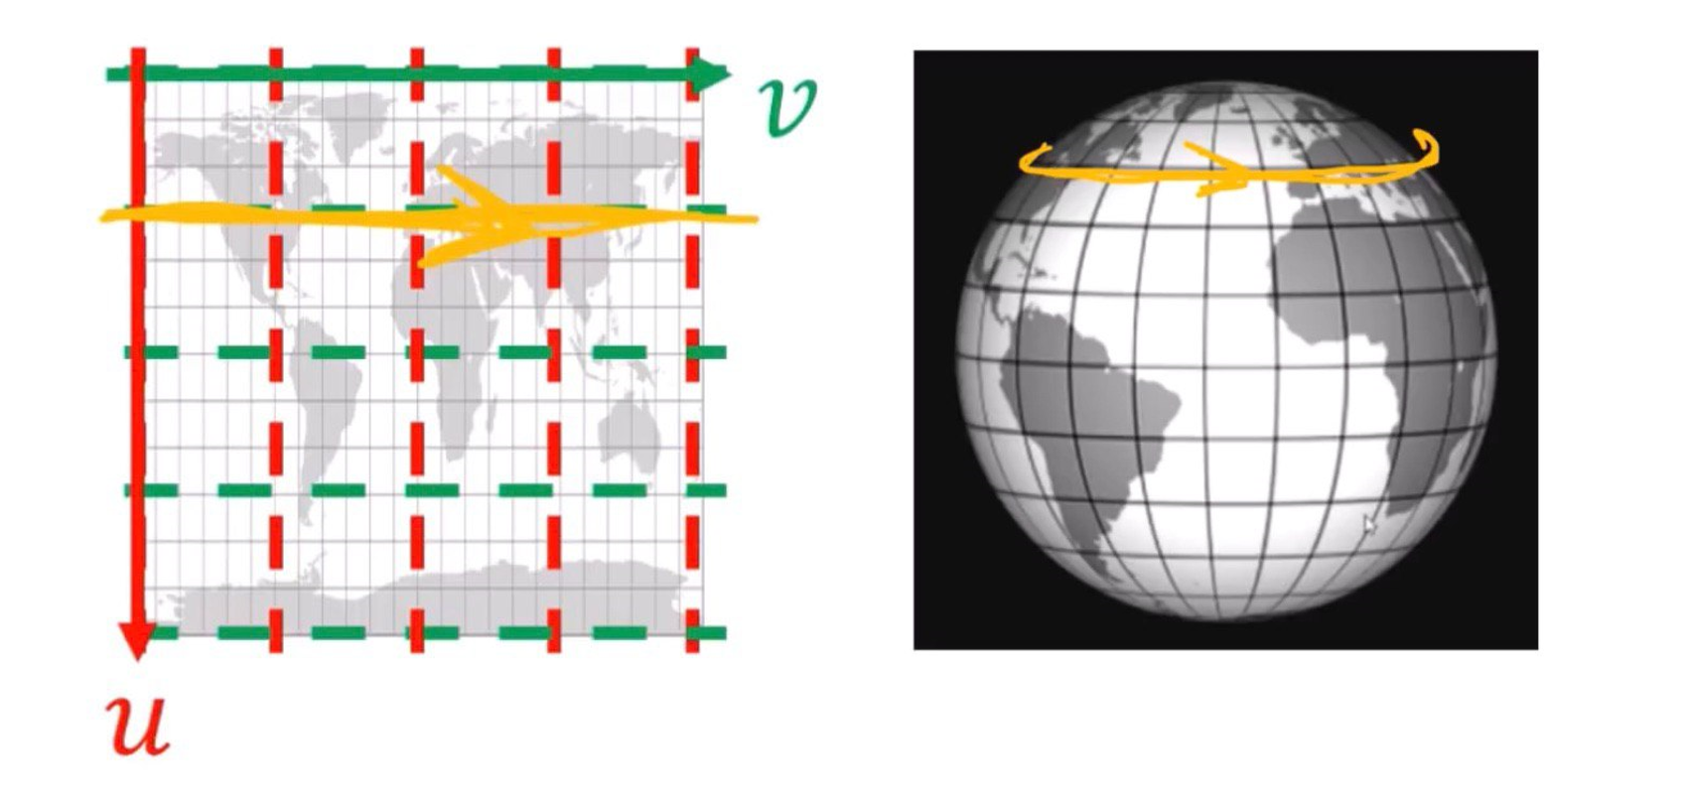
\includegraphics[scale=0.3]{figure/tropic.png}
        \caption{$u=\frac{\pi}{4},v=\lambda$}
    \end{figure}
    \item For $u=\frac{\pi}{2},v=\lambda$
    \begin{align*}
         \left\|\frac{d\vec R}{d\lambda}\right\|^2&=\left(\frac{du}{d\lambda}\right)^2+\sin^2(u)\left(\frac{dv}{d\lambda}\right)^2\\
         &=0^2+\sin^2\left(\frac{\pi}{2}\right)\cdot1^2=1
    \end{align*}
    The functional of arc length is
    \begin{equation*}
        \text{arc length}=\int\left\|\frac{d\vec R}{d\lambda}\right\|dt=\int1dt=t
    \end{equation*}
    \begin{figure}[H]
        \centering
        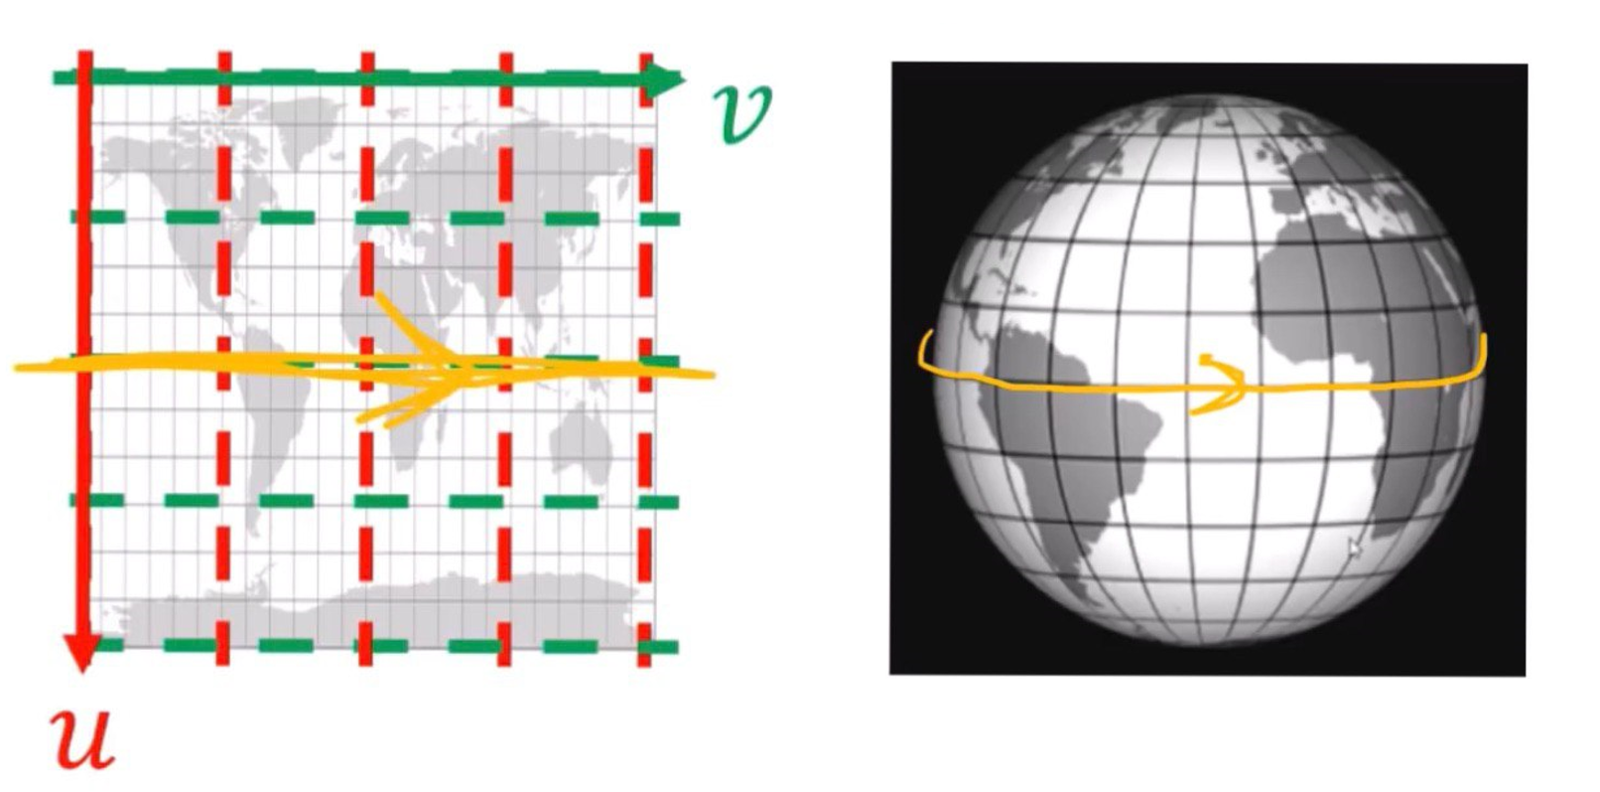
\includegraphics[scale=0.3]{figure/equator.png}
        \caption{$u=\frac{\pi}{2},v=\lambda$}
    \end{figure}
\end{itemize}
\end{example}
\begin{remark}
So the figure below is a good illustration of the role metric tensor plays:
\begin{figure}[H]
    \centering
    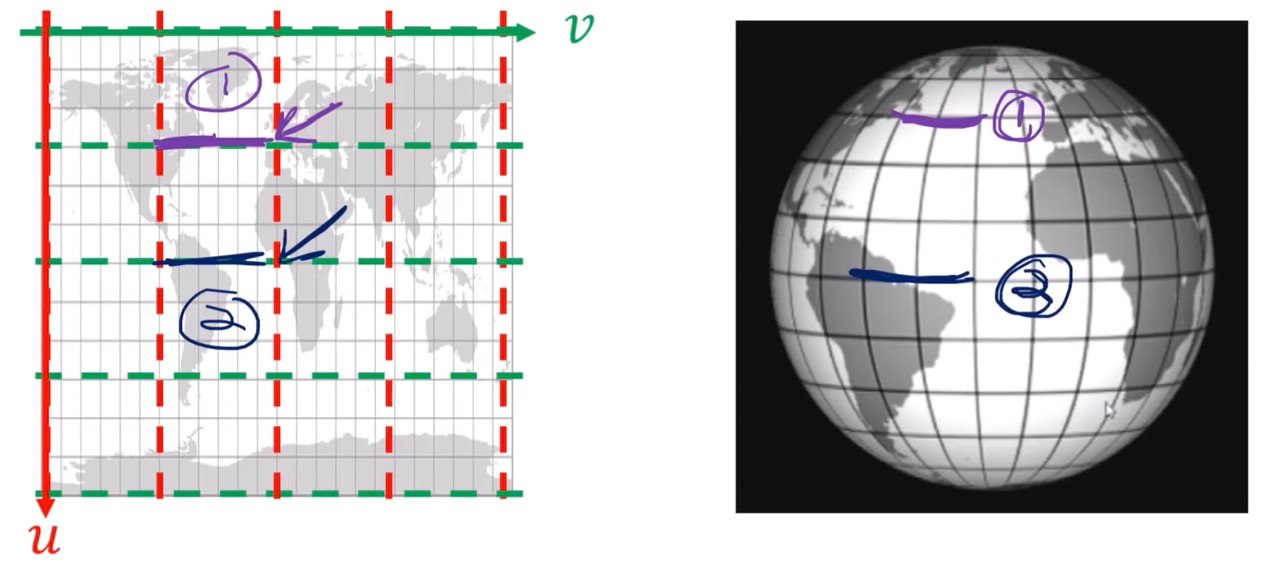
\includegraphics[scale=0.2]{figure/compare.jpg}
    \caption{What we usually see in expression convenience vs. What actually it is}
\end{figure}

The sub-figure left is what we usually see in practice, which gives us the illusion that this is an Euclidean space, but a distorted one. However, the actual shape of the manifold is the sub-figure right, which can be more arbitrary than this sphere in most cases. So, if we want to measure the distance between two points, what we need is simply the metric tensor on each points. With the metric tensor, we can derive the inner product of the velocity vector, then integrate the norm of velocity by $t$, we can have the distance we want.

In other words, the metric tensor is the tool to describe the shape of a manifold.
\end{remark}
\begin{remark}
As figure 11 shows, longer axis stands for higher time cost, while shorter axis represents lower time cost, namely a shorter distance. And figure 12 illustrates the previous property well - the closer to the polars, the lower time cost would be.
\end{remark}
\begin{figure}[H]
    \label{fig:metricinellipse}
    \centering
    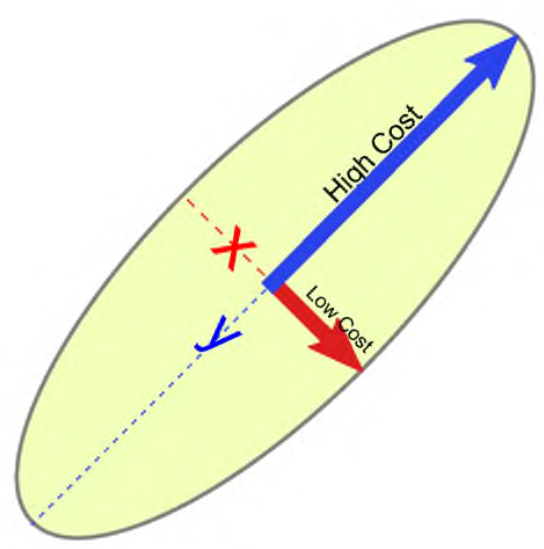
\includegraphics[scale=0.3]{figure/metricinellipse.png}
    \caption{Visualization of metric tensor}
\end{figure}

\begin{figure}[H]
    \label{fig:spheremetrictensor}
    \centering
    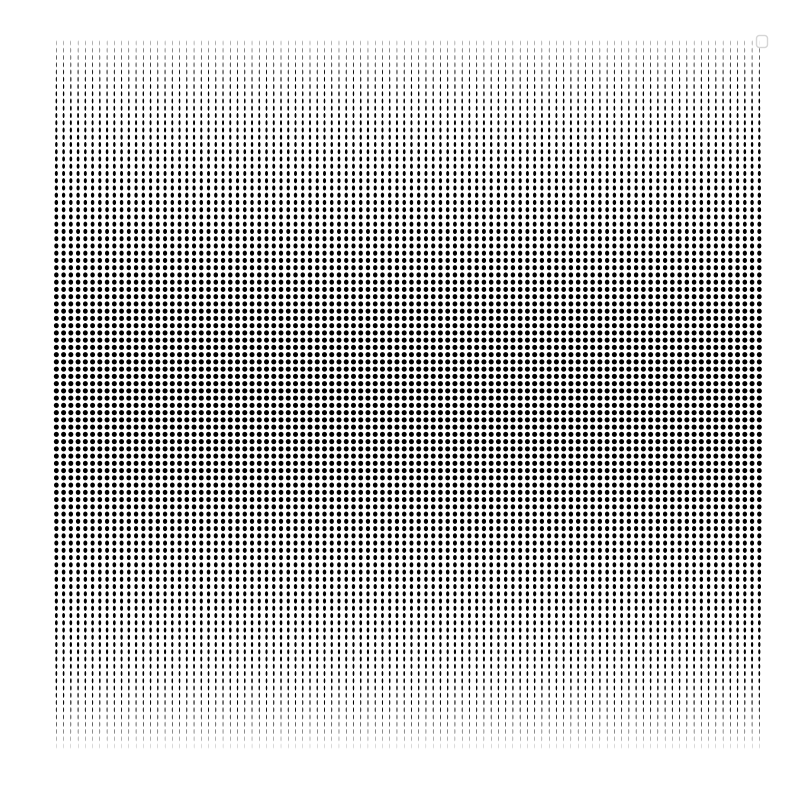
\includegraphics[scale=0.25]{figure/spheremetrictensor.png}
    \caption{Visualization of sphere metric field}
\end{figure}

\begin{definition} 
\boxed{\textbf{Riemannian manifold}} is a differentiable(smooth) manifold equipped with a Riemannian metric. 
\end{definition}

\begin{example}
The Riemannian metric can be equated with a smoothly varying positive-definite symmetric matrix $g$, called the metric tensor, defined at each point. For two vectors $v,w\in T_pM$, given local coordinates $(x^1, x^2,\cdots,x^n)$ in a neighborhood of $p$, the entry in $g$ ($n\times n$ matrix) can be expressed like below
\begin{equation*}
    g_{ij}=\langle E_i,E_j\rangle,
\end{equation*}
where $E_i=\frac{\partial}{\partial x^i}$ are the coordinate basis vectors at $p$. With this definition, we can compute the inner product $\langle v,w\rangle$ as $v^Tgw$. Also, for a vector $v$, we can compute the length of the vector as $\langle v,v\rangle^\frac{1}{2}$, which is the $L^2$ norm. Sometimes, people utilize the inverse of the diffusion tensor, $D^{-1}$, to define a local cost function as
\begin{equation*}
    \langle v,w\rangle=v^TD^{-1}w,
\end{equation*}
where $v, w\in T_pM$. In this case, since the inverse of the diffusion tensor are positive-definite symmetric and they are also Riemannian metric, a DTI is actually wrapped into a Riemannian manifold.
\end{example}

\begin{definition}
\boxed{\textbf{Runge–Kutta methods(RK4)}}

Let an initial value problem be specified as follows:
The only things we know are the slope of the tangent line to the curve $y$ at any point
\begin{equation*}
    \frac{dy}{dt}=f(t,y)
\end{equation*}
and the initial condition $(t_0,y_0)$, namely
\begin{equation*}
    y(t_0)=y_0.
\end{equation*}
We want to approximate the original function $y$, which equals to $\int f(t,y)$. For the $n+1^{th}$ iteration, we have the approximation
\begin{align*}
    y_{n+1}&=y_n+\frac{1}{6}h(k^n_1+2k^n_2+2k^n_3+k^n_4),\\
    t_{n+1}&=t_n+h,
\end{align*}
where $h$ is the step size and 
\begin{align*}
    k^n_1&=f(t_n,y_n)&&\triangleright \text{The slope at the beginning of the interval}\\
    k^n_2&=f\left(t_n+\frac{h}{2},y_n+h\frac{k^n_1}{2}\right)&&\triangleright \text{The slope at the midpoint of the interval, using $y$ and $k^n_1$}\\
    k^n_3&=f\left(t_n+\frac{h}{2},y_n+h\frac{k^n_2}{2}\right)&&\triangleright \text{The slope at the midpoint of the interval, using $y$ and $k^n_2$}\\
    k^n_4&=f(t_n+h,y_n+hk_3)&&\triangleright \text{The slope at the end of the interval, using $y$ and $k^n_3$}
\end{align*}
\end{definition}

\begin{remark}
When $k^n_4=k^n_3=k^n_2=k^n_1=f(t_n,y_n)$, it's the simplest Runge–Kutta method, namely the Euler method.
\end{remark}

\begin{remark}
In an ideal world, we can integrate a function by integration rules, like $\int e^x=e^x+c$. However, in the real world, we can only use a numerical procedure to integrate a random function. That's why we call the result of RK4 or Euler methods as integral curve, which is simply the result after integration.
\end{remark}

\begin{figure}[H]
    \centering
    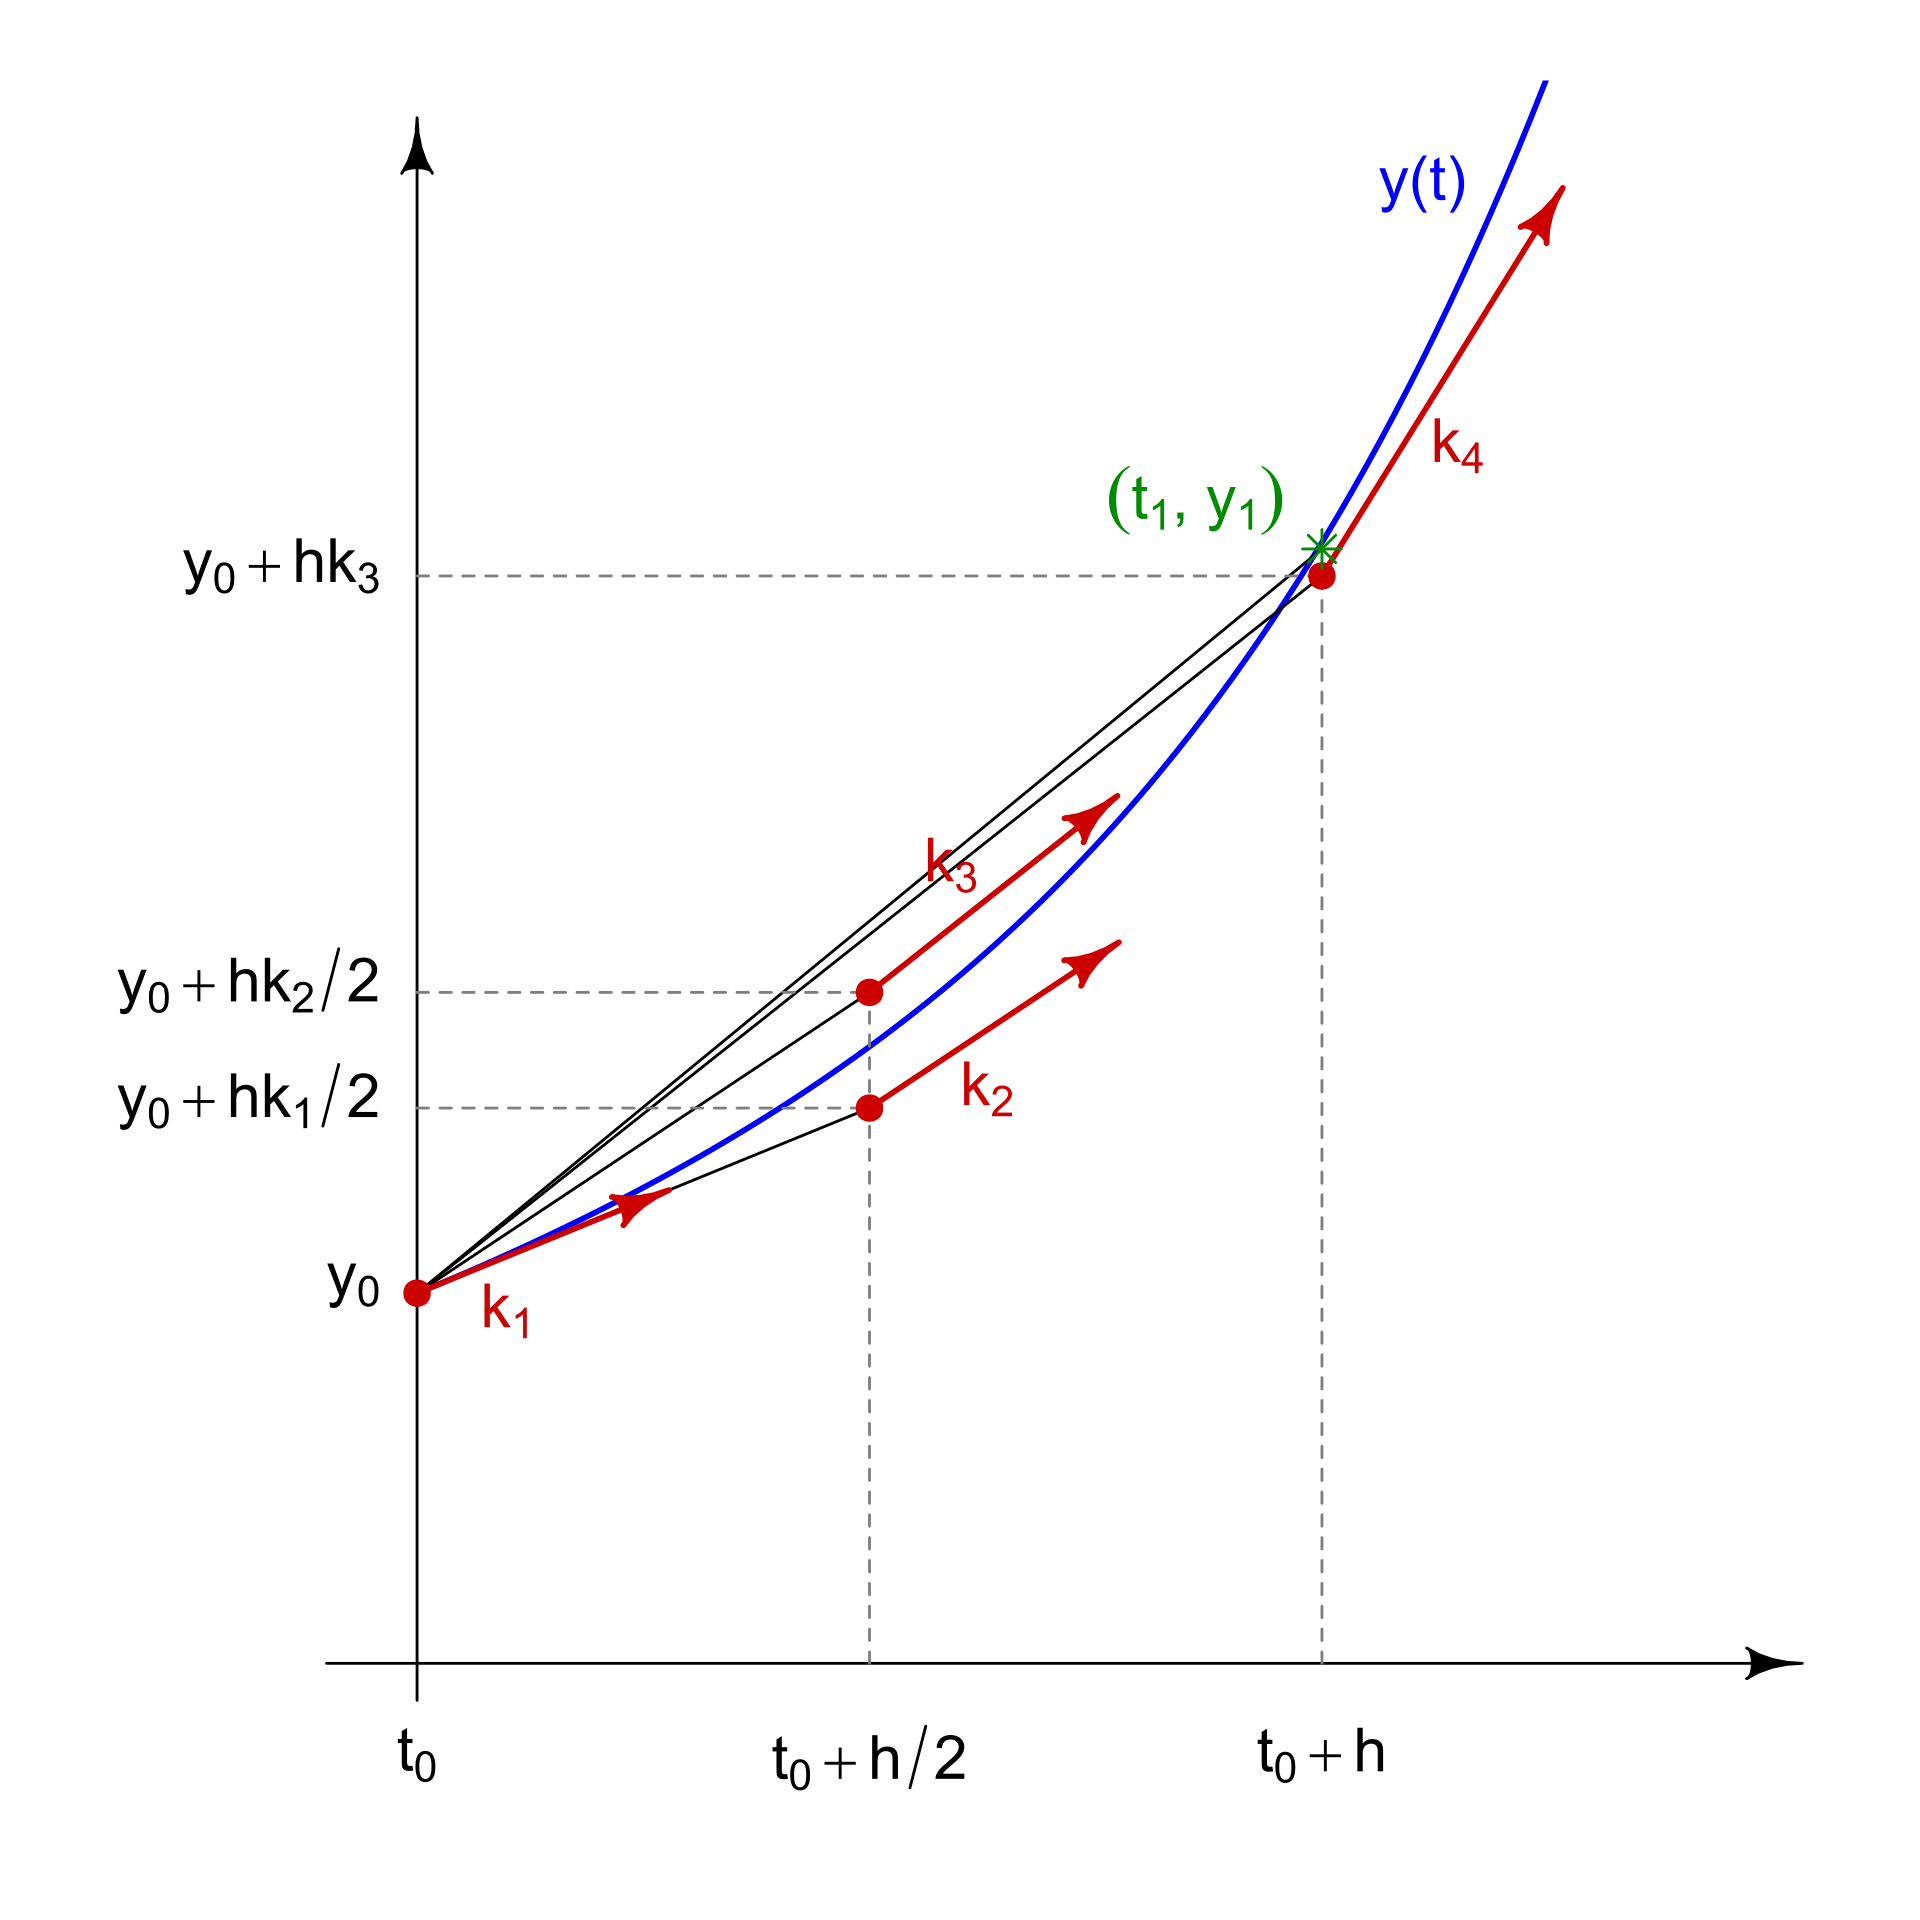
\includegraphics[scale=0.15]{figure/rk4.png}
    \caption{RK4}
\end{figure}

\begin{definition}
\boxed{\textbf{Integral curve}} is a parametric curve that represents a specific solution to an ordinary differential equation or system of equations. If the differential equation is represented as a vector field or slope field, then the corresponding integral curves are tangent to the field at each point.
\end{definition}

\begin{figure}[H]
  \centering
  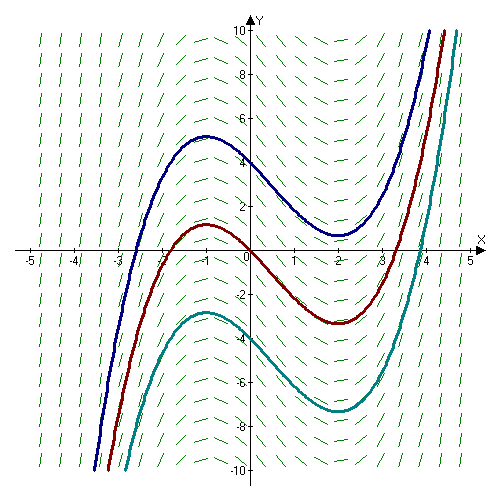
\includegraphics[scale=0.4]{figure/Slope_Field.png}
  \caption{Integral curve}
\end{figure}

\begin{definition}
\boxed{\textbf{Geodesic}} between two points $p,q\in M$ can be defined by the minimization of the energy functional
\begin{equation*}
    E(\gamma)=\int^1_0\|\Dot{\gamma}(t)\|^2dt
\end{equation*}
where $\gamma:[0,1]\rightarrow M$ is a curve with fixed endpoints $\gamma(0)=p, \gamma(1)=q$. The inner product between two tangent vectors $v,w\in T_xM$ is given by $\langle v,w\rangle=v^Tg(x)w$, where $g(x)$ is the Riemannian metric at point $x$.
\end{definition}

\begin{remark}\cite{stanford2}
\textbf{Intrinsic} distance is measured as ‘an ant would walk along the surface’. \textbf{Extrinsic} distance is defined as the $L^2$ norm between two points, basically ‘how a surface looks from the outside’. From the beginning and through the middle of the 18th century, differential geometry was studied from the extrinsic point of view: curves and surfaces were considered as lying in a Euclidean space of higher dimension. Starting with the work of Riemann, the intrinsic point of view was developed, in which one cannot speak of moving ``outside'' the geometric object because it is considered to be given in a free-standing way.
\end{remark}

\begin{example}\cite{bhatia}
Let $A$ and $B$ be any two elements of $\mathbb{P}^n$. Then there exists a unique geodesic $[A,B]$ joining $A$ and $B$. This geodesic has a parametrization
\begin{equation*}
    \gamma(t)=A^{\frac{1}{2}}(A^{-\frac{1}{2}}BA^{-\frac{1}{2}})^TA^{\frac{1}{2}}, t\in[0,1].
\end{equation*}
\end{example}

\begin{figure}[H]
   \centering
   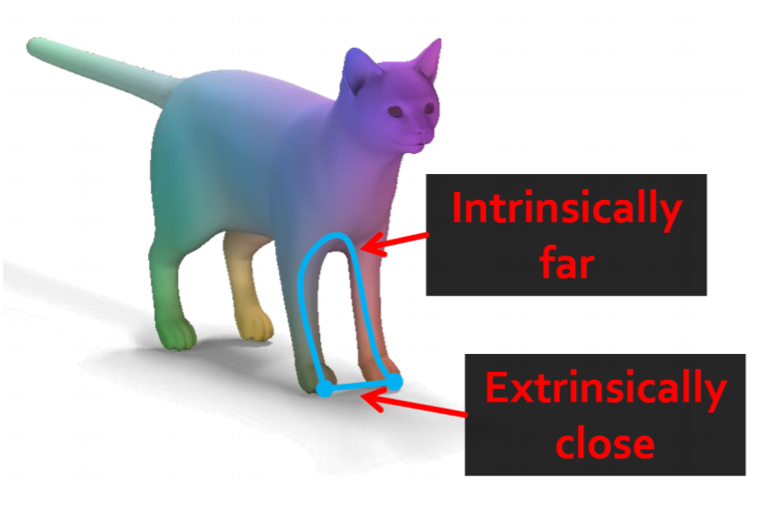
\includegraphics[scale=0.4]{figure/intrinsic.png}
   \caption{Intrinsic vs. Extrinsic Distance}
\end{figure}

\begin{definition}
\boxed{\textbf{Geodesic Equation}} guarantees the acceleration vector normal to the surface
\begin{equation*}
    \frac{d^2u^k}{dt^2}+\Gamma_{ij}^k\frac{du^i}{dt}\cdot\frac{du^j}{dt}=0
\end{equation*}
\end{definition}

\begin{proof}
In this section, all the computations are conducted in 2D situation.
\begin{align*}
    \text{Velocity Vector: }&\frac{d\vec{R}}{dt}=\frac{\partial\vec{R}}{\partial u}\cdot\frac{du}{dt}+\frac{\partial\vec{R}}{\partial v}\cdot\frac{dv}{dt}\\
    \text{Acceleration Vector: }&\frac{d^2\vec{R}}{dt^2}=\frac{d}{dt}\left(\frac{\partial\vec{R}}{\partial u}\cdot\frac{du}{dt}+\frac{\partial\vec{R}}{\partial v}\cdot\frac{dv}{dt}\right)
\end{align*}

Expend the expression of acceleration vector, we have
\begin{align*}
    \frac{d^2\vec{R}}{d t^2}&=\frac{d}{dt}\left(\frac{\partial\vec{R}}{\partial u}\cdot\frac{du}{dt}+\frac{\partial\vec{R}}{\partial v}\cdot\frac{dv}{dt}\right)\\
    &=\frac{\partial\vec{R}}{\partial u}\cdot\frac{d^2u}{dt^2}+\frac{du}{dt}\left(\frac{d}{dt}\cdot\frac{\partial\vec{R}}{\partial u}\right)+\frac{\partial\vec{R}}{\partial v}\cdot\frac{d^2v}{dt^2}+\frac{dv}{dt}\left(\frac{d}{dt}\cdot\frac{\partial\vec{R}}{\partial v}\right)\\
    &=\frac{\partial\vec{R}}{\partial u}\cdot\frac{d^2u}{dt^2}+\frac{du}{dt}\left(\frac{\partial}{\partial u}\cdot\frac{d\vec{R}}{d t}\right)+\frac{\partial\vec{R}}{\partial v}\cdot\frac{d^2v}{dt^2}+\frac{dv}{dt}\left(\frac{\partial}{\partial v}\cdot\frac{d\vec{R}}{dt}\right)\\
    &=\frac{\partial\vec{R}}{\partial u}\cdot\frac{d^2u}{dt^2}+\frac{du}{dt}\left[\frac{\partial}{\partial u}\cdot\left(\frac{\partial\vec{R}}{\partial u}\cdot\frac{du}{dt}+\frac{\partial\vec{R}}{\partial v}\cdot\frac{dv}{dt}\right)\right]\\
    &+\frac{\partial\vec{R}}{\partial v}\cdot\frac{d^2v}{dt^2}+\frac{dv}{dt}\left[\frac{\partial}{\partial v}\cdot\left(\frac{\partial\vec{R}}{\partial u}\cdot\frac{du}{dt}+\frac{\partial\vec{R}}{\partial v}\cdot\frac{dv}{dt}\right)\right]\\
    &=\frac{\partial \vec{R}}{\partial u}\cdot\frac{d^2 u}{d t^2}+\frac{\partial^2\vec{R}}{\partial u^2}\cdot\left(\frac{du}{dt}\right)^2+\frac{\partial^2\vec{R}^2}{\partial u\partial v}\cdot\frac{du}{dt}\cdot\frac{dv}{dt}\\
    &+\frac{\partial \vec{R}}{\partial v}\cdot\frac{d^2 v}{d t^2}+\frac{\partial^2\vec{R}^2}{\partial u\partial v}\cdot\frac{du}{dt}\cdot\frac{dv}{dt}+\frac{\partial^2\vec{R}}{\partial v^2}\cdot\left(\frac{dv}{dt}\right)^2
\end{align*}

By using Einstein Notation, and making $u^1=u, u^2=v$, we can denote the \textbf{acceleration vector} as 
\begin{equation}
    \boxed{\frac{d^2\vec{R}}{d t^2}=\frac{d^2 u^i}{d t^2}\cdot\frac{\partial \vec{R}}{\partial u^i}+\frac{du^i}{dt}\cdot\frac{du^j}{dt}\cdot\frac{\partial^2\vec{R}}{\partial u^i\partial u^j}}\label{eq10}
\end{equation}

Assuming that $\frac{\partial^2\vec{R}}{\partial u^i\partial u^j}$ is consist of three components, so we can express it like
\begin{equation*}
    \frac{\partial^2\vec{R}}{\partial u^i\partial u^j}=\Gamma_{ij}^1\frac{\partial \vec{R}}{\partial u^1}+\Gamma_{ij}^2\frac{\partial \vec{R}}{\partial u^2}+L_{ij}\vec{n}
\end{equation*}
where the Christoffel symbol $\Gamma_{ij}^k$, gives us the tangential component of $\frac{\partial^2\vec{R}}{\partial u^i\partial u^j}$ and the second fundamental form $L_{ij}$, gives us the normal component of $\frac{\partial^2\vec{R}}{\partial u^i \partial u^j}$. By using the Einstein Notation, we can have a more concise form as below:
\begin{equation}
    \boxed{\frac{\partial^2\vec{R}}{\partial u^i\partial u^j}=\Gamma_{ij}^k\frac{\partial \vec{R}}{\partial u^k}+L_{ij}\vec{n}}\label{eq9}
\end{equation}

\begin{figure}[H]
   \centering
   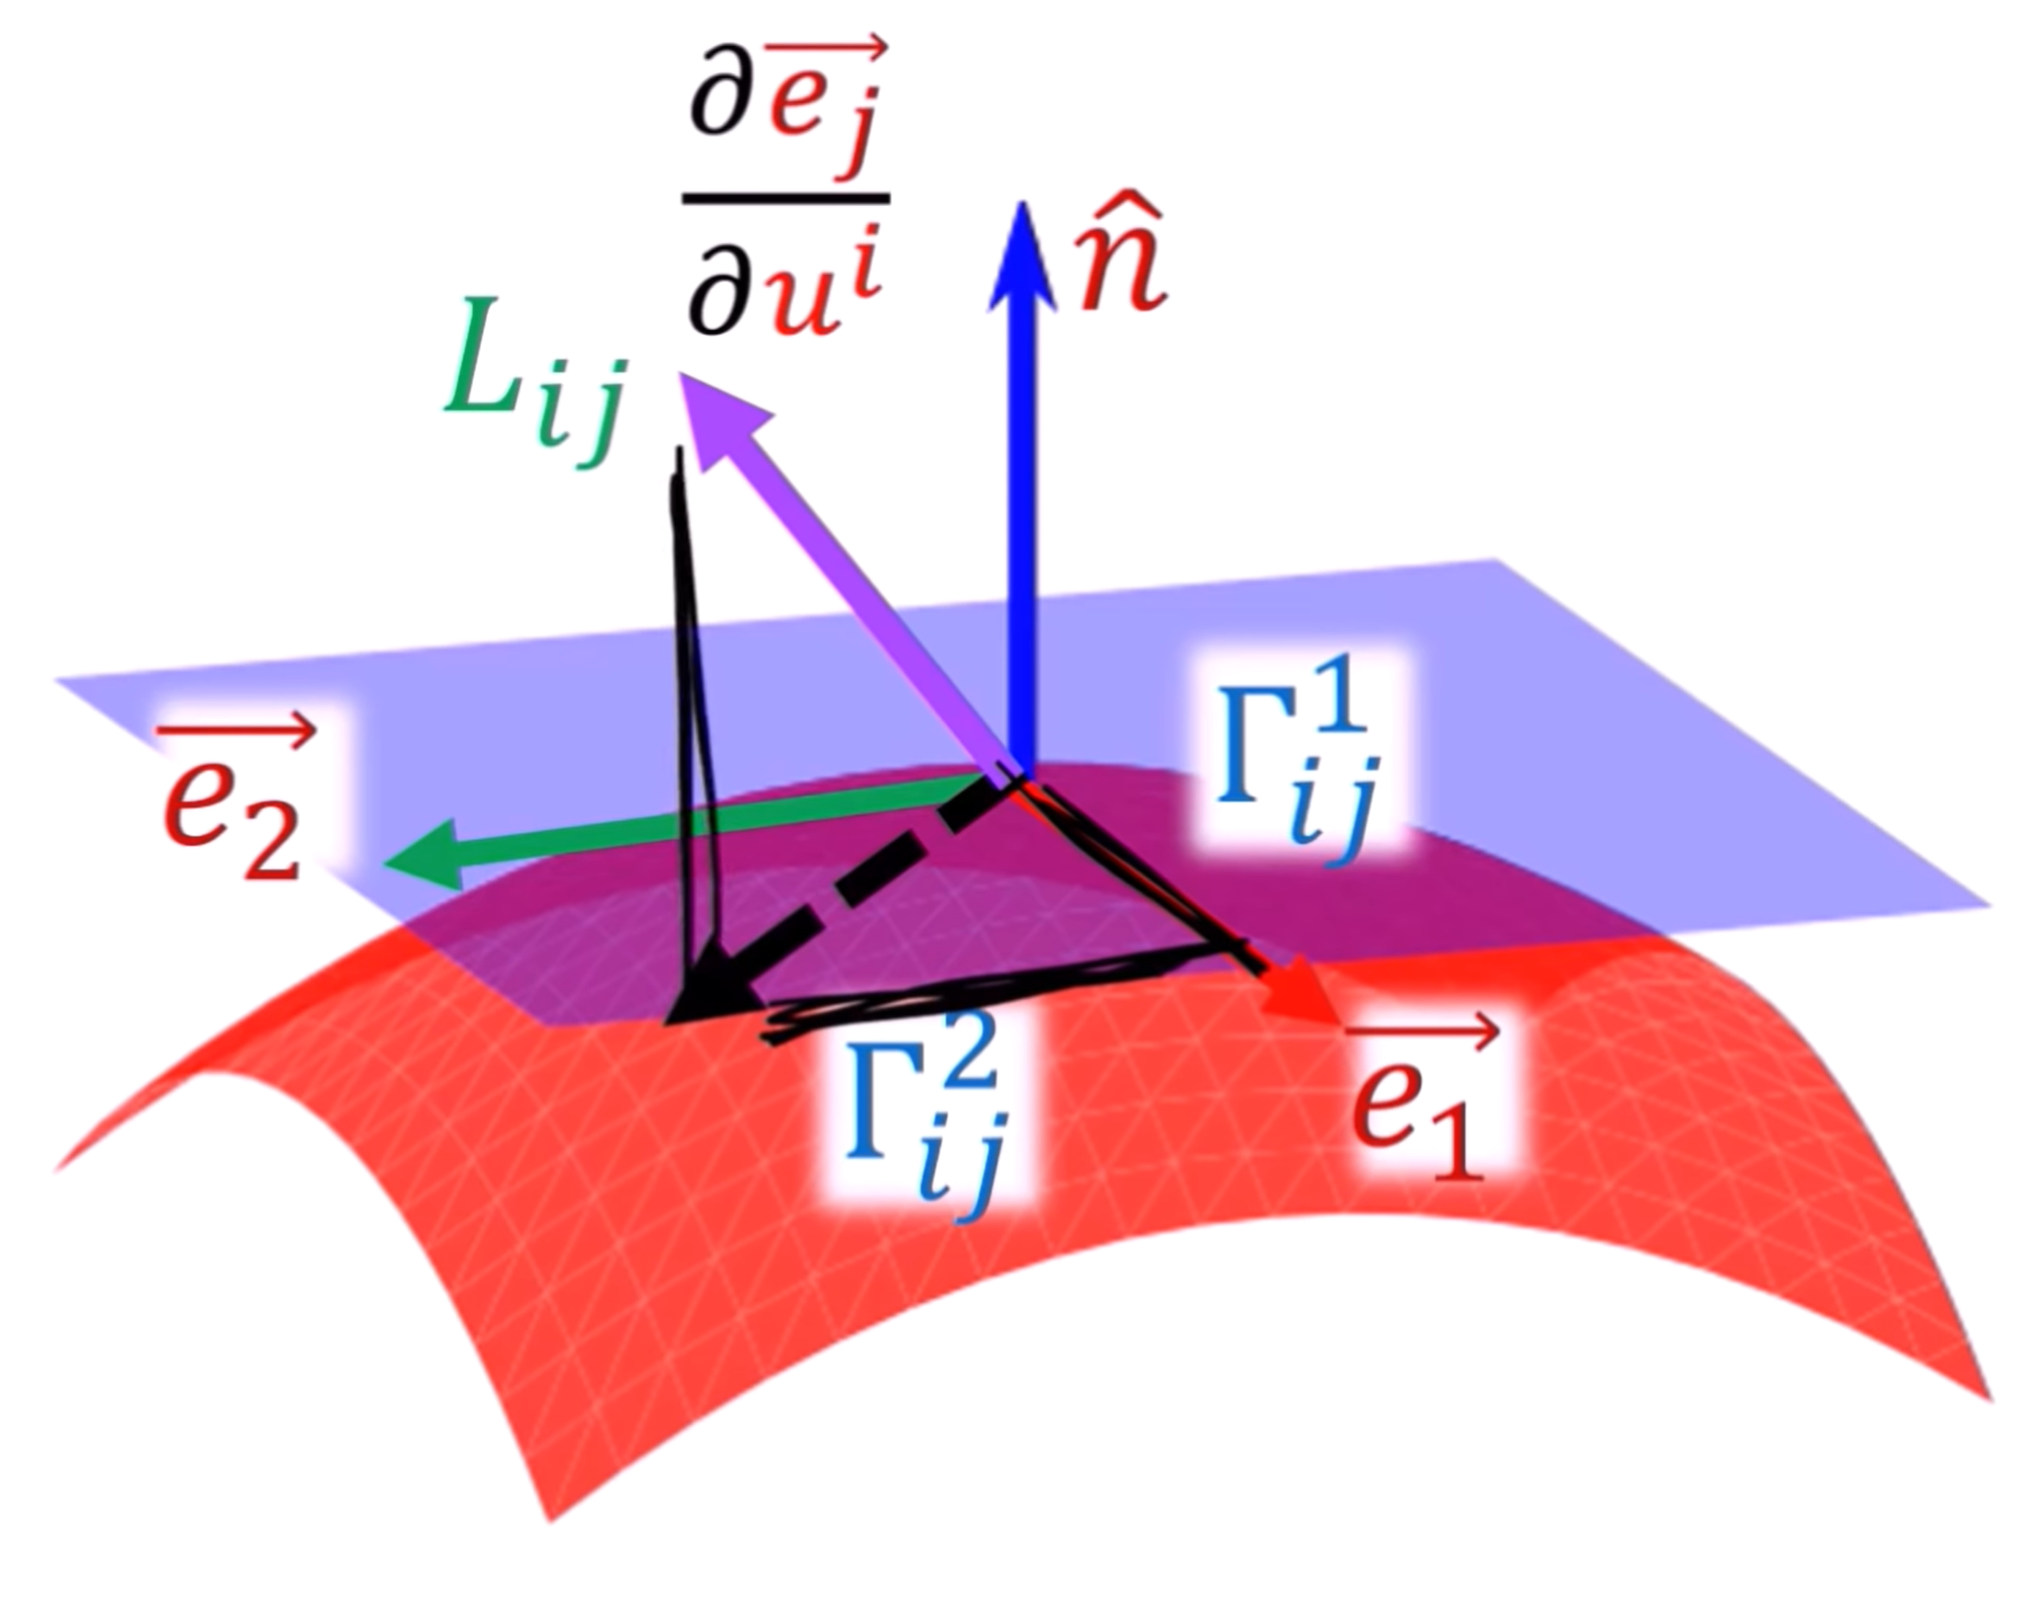
\includegraphics[scale=0.13]{figure/christoffel.png}
   \caption{meaning of $L_{ij},\Gamma^k_{ij}$}
\end{figure}

Finally, by substituting Eq.(\ref{eq9}) into Eq.(\ref{eq10}), we can have acceleration vector as below
\begin{align*}
    \frac{d^2\vec{R}}{dt^2}&=\frac{d^2 u^i}{d t^2}\cdot\frac{\partial \vec{R}}{\partial u^i}+\frac{du^i}{dt}\cdot\frac{du^j}{dt}\cdot\frac{\partial^2\vec{R}}{\partial u^i\partial u^j}\\
    &=\frac{d^2 u^i}{d t^2}\cdot\frac{\partial \vec{R}}{\partial u^i}+\frac{du^i}{dt}\cdot\frac{du^j}{dt}\cdot\left(\Gamma_{ij}^k\frac{\partial \vec{R}}{\partial u^k}+L_{ij}\vec{n}\right)\\
    &=\underbrace{\left(\frac{d^2u^k}{dt^2}+\Gamma_{ij}^k\frac{du^i}{dt}\cdot\frac{du^j}{dt}\right)\frac{\partial\vec{R}}{\partial u^k}}_{\text{tangential part}}+\underbrace{L_{ij}\cdot\frac{du^i}{dt}\cdot\frac{du^j}{dt}\cdot\vec{n}}_{\text{normal part}}
\end{align*}

That acceleration vector normal to the surface requires
\begin{equation*}
    \frac{d^2u^k}{dt^2}+\Gamma_{ij}^k\frac{du^i}{dt}\cdot\frac{du^j}{dt}=0,
\end{equation*}
which is the Geodesic Equation.

\paragraph{Derivation of $\Gamma_{ij}^k$ and $L_{ij}$}
As $\vec{n}$ is perpendicular to the tangent vectors, therefore, by multiplying $\frac{\partial\vec{R}}{\partial u^l}$ on both sides of equation above, we can yield that
\begin{equation}
    \frac{\partial^2\vec{R}}{\partial u^i\partial u^j}\cdot\frac{\partial\vec{R}}{\partial u^l}=\left(\Gamma_{ij}^k\frac{\partial \vec{R}}{\partial u^k}+L_{ij}\vec{n}\right)\cdot\frac{\partial\vec{R}}{\partial u^l}=\Gamma_{ij}^k\frac{\partial \vec{R}}{\partial u^k}\cdot\frac{\partial\vec{R}}{\partial u^l}\label{eq8}
\end{equation}

Since $\frac{\partial \vec{R}}{\partial u^k}\cdot\frac{\partial\vec{R}}{\partial u^l}=\vec{e}_k\cdot\vec{e}_l=g_{kl}$, then we get
\begin{equation*}
    \frac{\partial^2\vec{R}}{\partial u^i\partial u^j}\cdot\frac{\partial\vec{R}}{\partial u^l}=\Gamma_{ij}^kg_{kl},
\end{equation*}

By substituting the metric form below into Eq.(\ref{eq8})
\begin{equation*}
    \begin{pmatrix}
        \frac{\partial\vec{R}}{\partial u^1}\cdot\frac{\partial\vec{R}}{\partial u^1} & \frac{\partial\vec{R}}{\partial u^1}\cdot\frac{\partial\vec{R}}{\partial u^2} \\
        \frac{\partial\vec{R}}{\partial u^2}\cdot\frac{\partial\vec{R}}{\partial u^1} & \frac{\partial\vec{R}}{\partial u^2}\cdot\frac{\partial\vec{R}}{\partial u^2}
    \end{pmatrix}
    =
    \begin{pmatrix}
        g_{11} & g_{12} \\
        g_{21} & g_{22}
    \end{pmatrix}
\end{equation*}
and with Kronecker delta cancellation rule $g_{kl}\cdot g^{lm}=\delta_k^m$, we can have
\begin{align}
    \Gamma_{ij}^kg_{kl}g^{lm}&=\frac{\partial^2\vec{R}}{\partial u^i\partial u^j}\cdot\frac{\partial\vec{R}}{\partial u^l}\cdot g^{lm}\nonumber\\
    \Gamma_{ij}^k\delta_k^m&=\frac{\partial^2\vec{R}}{\partial u^i\partial u^j}\cdot\frac{\partial\vec{R}}{\partial u^l}\cdot g^{lm}\nonumber\\
    \Gamma_{ij}^m&=\left(\frac{\partial\Vec{e_j}}{\partial u^i}\cdot\Vec{e_l}\right)g^{lm}\label{chrisex}
\end{align}

Likewise, by multiplying $\vec{n}$ at both side of Eq.(\ref{eq9}), we can yield the extrinsic expression of second fundamental form
\begin{equation*}
    L_{ij}=\frac{\partial^2\vec{R}}{\partial u^i\partial u^j}\cdot \vec{n}
\end{equation*}
\end{proof}

\begin{definition}
Given a vector space $V$ and a functional $f:V\rightarrow\mathbb{R}$, $x,h\in V, \alpha\in\mathbb{R}$, if the limit
\begin{equation*}
    \delta f(x)=\lim_{\alpha\rightarrow0}\frac{1}{\alpha}[f(x+\alpha h)-f(x)]
\end{equation*}
exists, it's called the \boxed{\textbf{G\^ateaux derivative}} of $f$ at $x$ with increment $h$. If the limit exists for $\forall h\in V$, the functional $f$ is said to be G\^ateaux differentiable at $x$.
\end{definition}
\begin{example}
Given $x\in\mathbb{R}^n$ and $f:\mathbb{R}^n\rightarrow\mathbb{R}$, which has continuous partial derivatives with respect to each components of $x$. Then, the Gateaux derivative of $f$ is
\begin{equation*}
    \delta f(x)=\sum^n_{i=1}\frac{\partial f}{\partial x_i}h_i=\langle\nabla f,h\rangle
\end{equation*}
\end{example}

\begin{definition}
\boxed{\textbf{Directional derivative}} of a multivariate differentiable function along a given vector $v$ at a given point $x$ intuitively represents the instantaneous rate of change of the function, moving through $x$ with a velocity specified by $h$.
\begin{equation*}
    \nabla_hf(x)=Df(x)(h)=\langle\nabla f,h\rangle
\end{equation*}
\end{definition}

\begin{remark}
Relationship between \textbf{partial derivative(scalar), directional derivative(scalar) and gradient(vector)}:
\begin{itemize}
    \item The vector consists of partial derivatives is the gradient.
    \item The linear combination of partial derivatives is directional derivative.
    \item Partial derivative is a special directional derivative, which is along the axis.
\end{itemize}
\end{remark}

\begin{remark}
Relationship between \textbf{G\^ateaux derivative(scalar), directional derivative(scalar) and covariant derivative(vector)}:
\begin{itemize}
    \item G\^ateaux derivative(differential) is a generalization of the concept of directional derivative in differential calculus.
    \item Covariant derivative is a generalization of the directional derivative from vector calculus. The covairant derivative of a function is directional 
    \item G\^ateaux and directional derivative are applicable to functional $f:\mathbb{R}^n\rightarrow\mathbb{R}$, so their output are both scalars. While the covariant derivative is for vector field $v:\mathbb{R}^n\rightarrow\mathbb{R}^n$, so its output is still a vector.
\end{itemize}
\end{remark}

\begin{align*}
    \nabla_hf(x)&=h^i\nabla_{\frac{\partial}{\partial x^i}}f\\
    &=h^i\frac{\partial f}{\partial x^i}
\end{align*}

\begin{align*}
    \nabla_hv&=h^i\nabla_{\frac{\partial}{\partial u^i}}(v^j \vec{e_j})\\
    &=h^i\left(\frac{\partial v^j}{\partial u^i}\vec{e_j}+v^j\nabla_{\frac{\partial}{\partial u^i}}\vec{e_j}\right)\\
    &=h^i\left(\frac{\partial v^j}{\partial u^i}\vec{e_j}+v^j\frac{\partial \vec{e_j}}{\partial u^i}\right)\\
    &=h^i\left(\frac{\partial v^j}{\partial u^i}\vec{e_j}+v^j\Gamma^k_{ij}\vec{e_k}\right) && \triangleright  \frac{\partial\vec{e_j}}{\partial u^i}=\Gamma^k_{ij}\vec{e_k}\\
    &=h^i\left(\frac{\partial v^k}{\partial u^i}\vec{e_k}+v^j\Gamma^k_{ij}\vec{e_k}\right)\\
    &=h^i\left(\frac{\partial v^k}{\partial u^i}+v^j\Gamma^k_{ij}\right)\vec{e_k}
\end{align*}

\begin{definition}
\boxed{\textbf{Covariant derivative}} $\nabla_{\vec{w}}\vec{v}$, refers to Levi-Civita connection generally,
\begin{itemize}
    \item is the ordinary derivative for Euclidean space.
    \item is the rate of change vector at $\Vec{v}$ of a vector field in a direction $\Vec{w}$ with the normal component subtracted, extrinsically.
\end{itemize}

Levi-Civita connection has following properties:
\begin{enumerate}
    \item $\nabla_{a\vec{w}+b\vec{t}}\vec{v}=a\nabla_{\vec{w}}\vec{v}+b\nabla_{\vec{t}}\vec{v}$
    \item $\nabla_{\vec{w}}(\vec{v}+\vec{u})=\nabla_{\vec{w}}\vec{v}+\nabla_{\vec{w}}\vec{u}$\Comment{Distributive Property}
    \item $\nabla_{\vec{w}}(\vec{v}\cdot\vec{u})=(\nabla_{\vec{w}}\vec{v})\cdot\vec{u}+\vec{v}\cdot(\nabla_{\vec{w}}\vec{u})$\Comment{Product Rule}
    \item $\nabla_{\vec{w}}(a\vec{v})=(\nabla_{\vec{w}}a)\vec{v}+a(\nabla_{\vec{w}}\vec{v})$
    \item $\nabla_{\partial_i}(a)=\frac{\partial a}{\partial u^i}$
    \item $\nabla_{\vec{w}}\vec{v}=\nabla_{\vec{v}}\vec{w}$\Comment{Commutative Property}
\end{enumerate}
\end{definition}

\begin{remark}
\begin{itemize}
    \item In Euclidean space, the covariant derivative is simply the change of the vector fields that take changing basis vectors into account.
    \item \textbf{Parallel transport} provides a way to compare a vector in one tangent plane to a vector in another, by moving the vector along a curve without changing it.
    \item Different expressions of $\Gamma^m_{kj}$ give us different ways of ``parallel transport''. If $\Gamma^m_{kj}=\frac{1}{2}g^{im}\left(\frac{\partial g_{ij}}{\partial u^k}+\frac{\partial g_{ki}}{\partial u^j}-\frac{\partial g_{jk}}{\partial u^i}\right)$, then it's Levi-Civita connection. If $\Gamma^m_{kj}=0$, it's another connection.
    \begin{figure}[H]
        \centering
        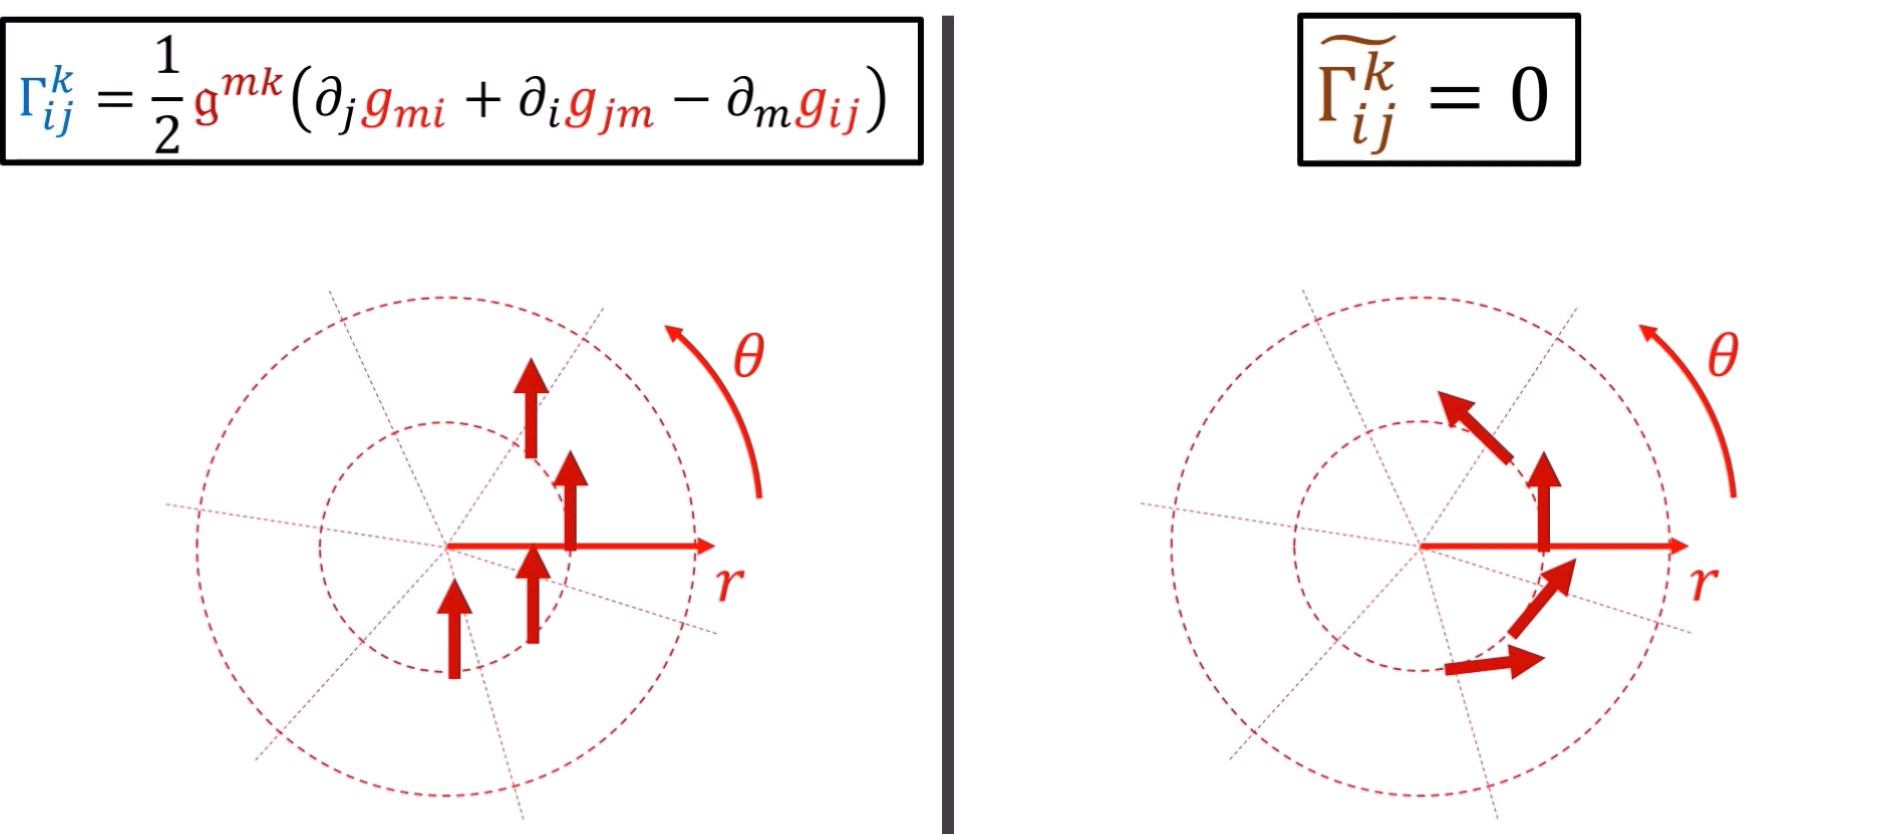
\includegraphics[scale=0.25]{figure/paralleltransport.png}
        \caption{Different definitions of $\Gamma^m_{kj}$ give us different kinds of ``parallel transport''.}
    \end{figure}
    \item Covariant derivative helps us find parallel transported vector fields. $\nabla_{\vec{w}}\vec{v}=\vec{0}$ means the vector $\Vec{v}$ is parallel transported in the direction $\Vec{w}$ at $\Vec{v}$'s position.
    \item \cite{rg} Covariant derivative $\nabla_{\vec{w}}\vec{v}$ is the difference between a vector field $v$ and its parallel transport in the direction $w$.
    \begin{figure}[H]
        \centering
        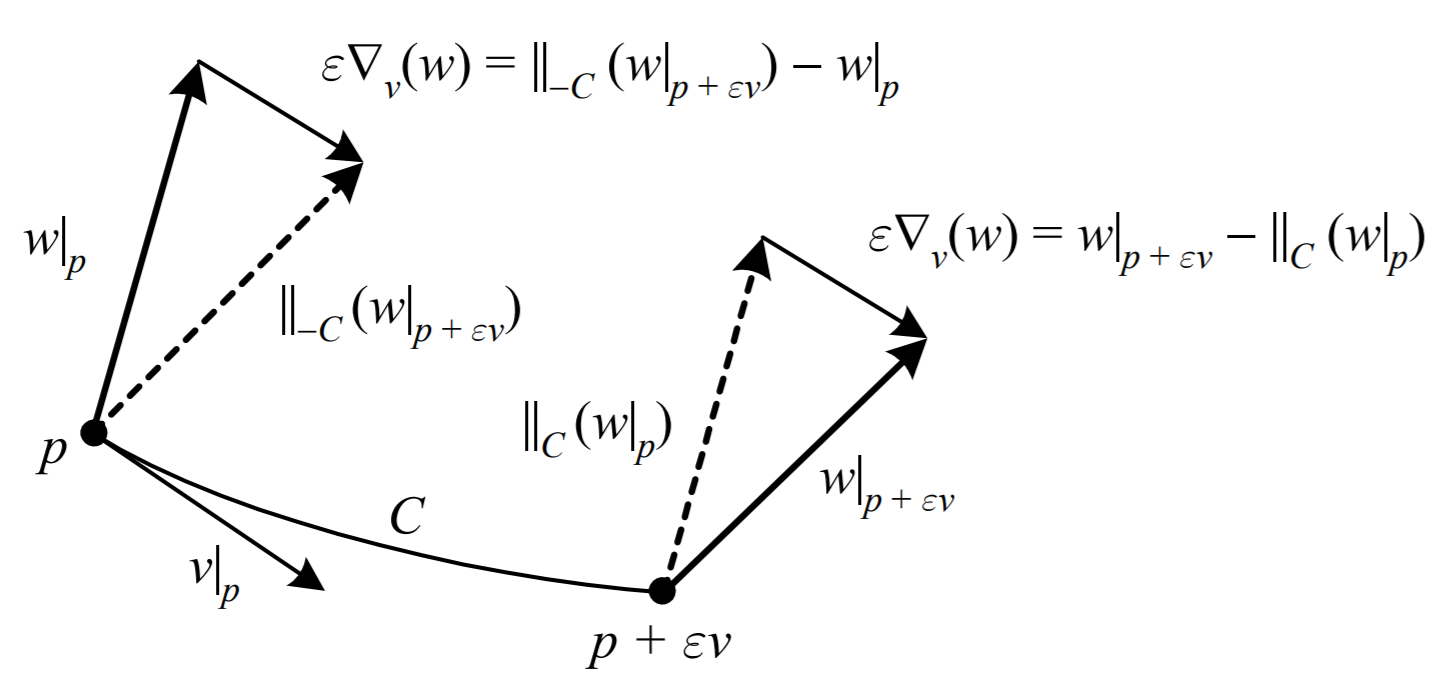
\includegraphics[scale=0.2]{figure/difference.png}
        \caption{Difference between a vector and the parallel transported one}
    \end{figure}
    \item Covariant derivative provides a connection between tangent spaces in a curved space.
    \item In curved space, a geodesic has zero tangential acceleration when we travel along it at constant speed. To compute geodesic curves, we need to find curves where the acceleration vector is normal to the space, namely $\nabla_{\Dot{\gamma}(t)}\Dot{\gamma}(t)=\vec{0}$ holds along the curve $\gamma$.
    \item In other words, geodesic is a curve resulting from parallel transporting a vector along itself.
\end{itemize}
\end{remark}

\begin{example}\cite{cd1}
In a 2D Euclidean space, we represent a vector as below:
\begin{equation*}
    \Vec{v}=v^1\Vec{e_1}+v^2\Vec{e_2}=\sum_iv^i\Vec{e_i}=v^i\Vec{e_i}, 
\end{equation*}
where $v^1,v^2$ are constant.
\begin{figure}[H]
   \centering
   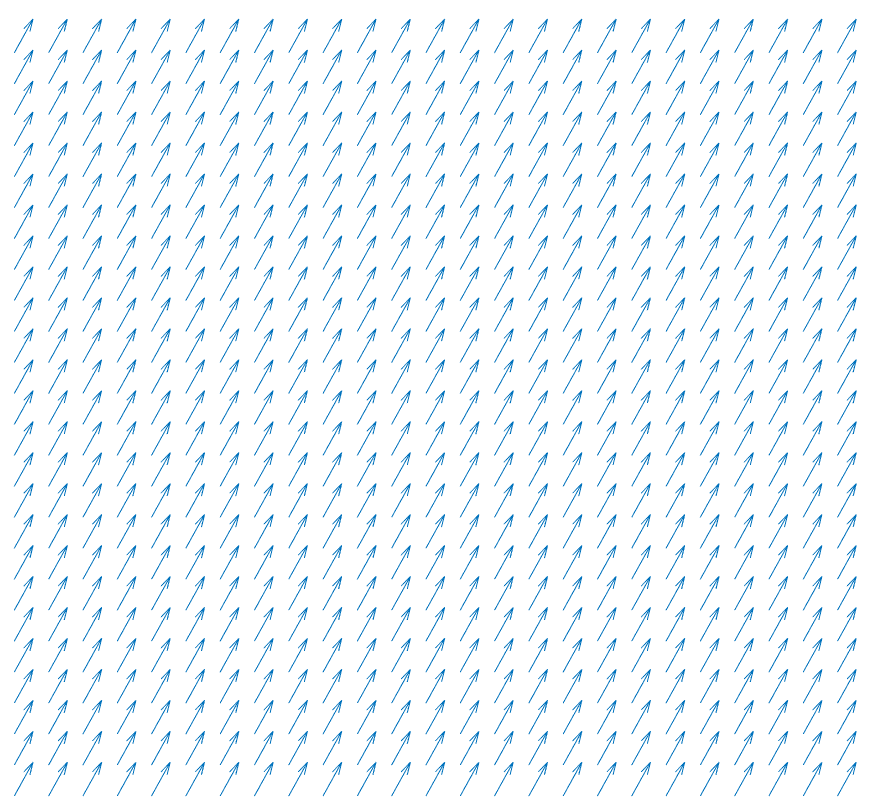
\includegraphics[scale=0.3]{figure/flatspace.png}
   \caption{Constant vector space}
\end{figure}

The covariant derivative defined in Euclidean space is just intuitive:
\begin{align*}
    \nabla_\frac{\partial}{\partial u^1}\Vec{v}&=\frac{\partial}{\partial u^1}\Vec{v}\\
    &=\frac{\partial}{\partial u^1}(v^1\Vec{e_1}+v^2\Vec{e_2})\\
    &=\frac{\partial}{\partial u^1}(v^1\Vec{e_1})+\frac{\partial}{\partial u^1}(v^2\Vec{e_2})\\
    &=\frac{\partial v^1}{\partial u^1}\Vec{e_1}+v^1\frac{\partial \Vec{e_1}}{\partial u^1}+\frac{\partial v^2}{\partial u^1}\Vec{e_2}+v^2\frac{\partial \Vec{e_2}}{\partial u^1}\\
    &=\frac{\partial v^1}{\partial u^1}\Vec{e_1}+\frac{\partial v^2}{\partial u^1}\Vec{e_2}\\
    &=\Vec{0}\\
    \nabla_\frac{\partial}{\partial u^2}\Vec{v}&=\frac{\partial}{\partial u^2}\Vec{v}\\
    &=\frac{\partial v^1}{\partial u^2}\Vec{e_1}+\frac{\partial v^2}{\partial u^2}\Vec{e_2}\\
    &=\Vec{0}
\end{align*}

In conclusion, in Euclidean space, the covariant derivative of a vector field is just the ordinary derivative. We need to make sure to differentiate both the vector components and the basis vectors.
\begin{align*}
    \frac{\partial}{\partial u^i}\Vec{v}&=\frac{\partial}{\partial u^i}v^j\Vec{e_j}\\
    &=\underbrace{\frac{\partial v^j}{\partial u^i}\Vec{e_j}}_{\text{components}}+\underbrace{\frac{\partial\Vec{e_j}}{\partial u^i}v^j}_{\text{basis vectors}}
\end{align*}
\end{example}

\begin{example}\cite{cd2}
In extrinsic case, the covariant derivative is defined as below
\begin{align}
    \nabla_\frac{\partial}{\partial u^i}\Vec{v}&=\frac{\partial\Vec{v}}{\partial u^i}-\Vec{n}\nonumber\\
    &=\frac{\partial}{\partial u^i}(v^1\Vec{e_1}+v^2\Vec{e_2})-\Vec{n}\nonumber\\
    &=\frac{\partial}{\partial u^i}v^j\Vec{e_j}-\Vec{n}\nonumber\\
    &=\frac{\partial v^j}{\partial u^i}\Vec{e_j}+\frac{\partial\Vec{e_j}}{\partial u^i}v^j-\Vec{n}\nonumber\\
    &=\frac{\partial v^j}{\partial u^i}\Vec{e_j}+(\Gamma^k_{ij}\Vec{e_k}+L_{ij}\hat{n})v^j-\Vec{n} && \triangleright  \frac{\partial\Vec{e_j}}{\partial u^i}=\Gamma^1_{ij}\Vec{e_1}+\Gamma^2_{ij}\Vec{e_2}+L_{ij}\hat{n}\nonumber\\
    &=\frac{\partial v^j}{\partial u^i}\Vec{e_j}+\Gamma^k_{ij}\Vec{e_k}v^j\nonumber\\
    &=\frac{\partial v^k}{\partial u^i}\Vec{e_k}+\Gamma^k_{ij}\Vec{e_k}v^j\nonumber\\
    &=\left(\frac{\partial v^k}{\partial u^i}+\Gamma^k_{ij}v^j\right)\Vec{e_k}\label{eq1}
\end{align}
where $L_{ij}$ is the second fundamental form and $\Gamma^k_{ij}$ is in form of Eq.(\ref{chrisex}).

Parameterize the space with tangent space basis
\begin{align*}
    \Vec{R}&=[X,Y,Z]^T\\
    \text{where }X&=\cos(u^2)\sin(u^1)\\
    Y&=\sin(u^2)\sin(u^1)\\
    Z&=\cos(u^1),
\end{align*}
where $\Vec{R}$ is the position vector and $u^1, u^2$ represents the latitude and longitude, respectively.

\begin{figure}[H]
   \centering
   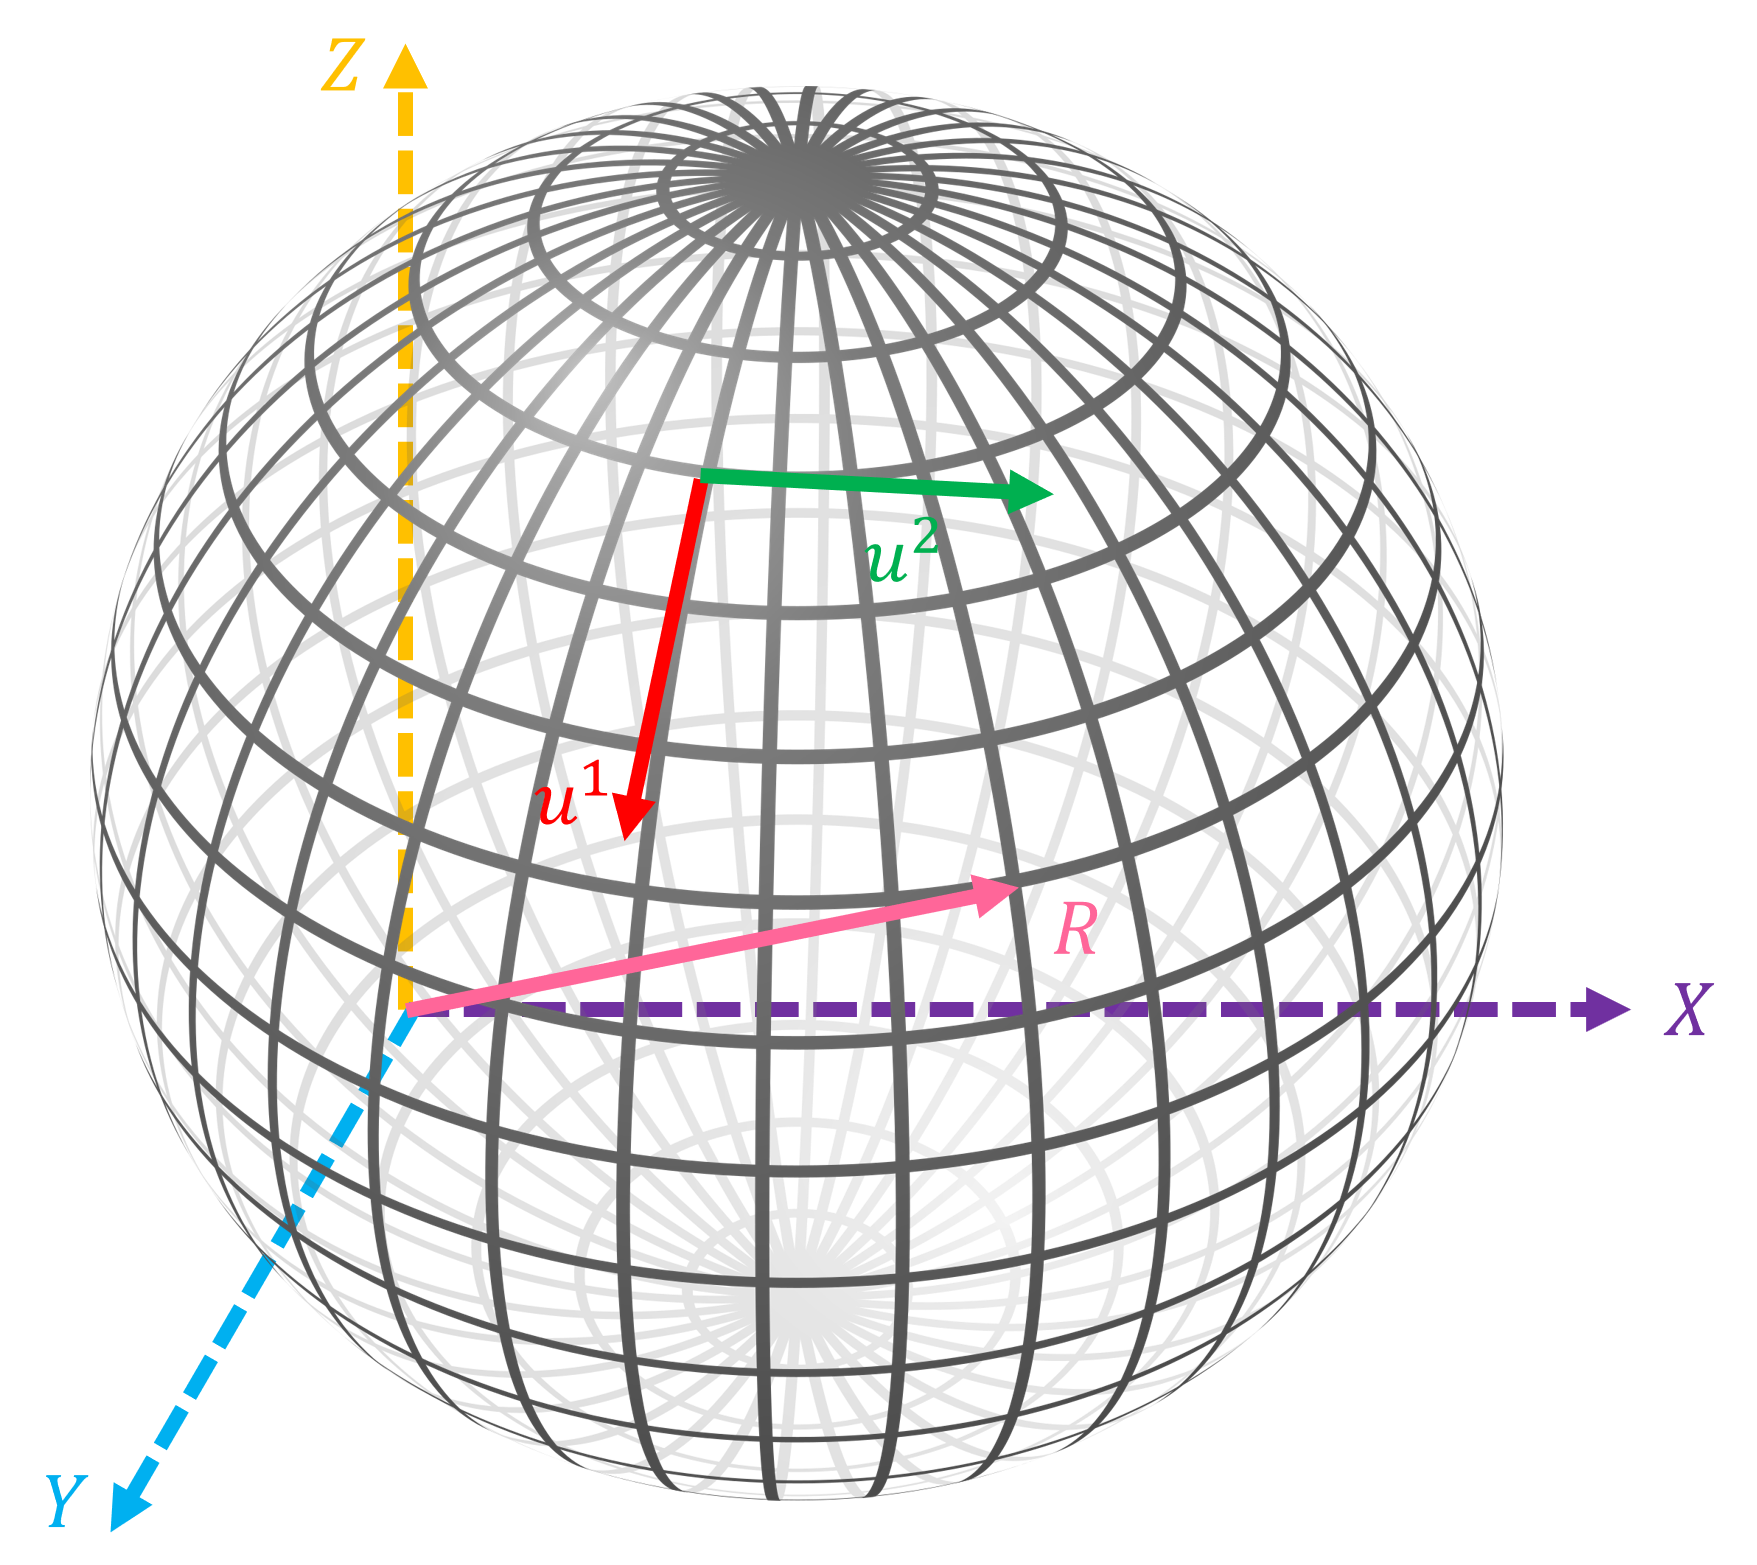
\includegraphics[scale=0.13]{figure/sphere.png}
   \caption{Parametric equations for sphere}
\end{figure}

By using the chain rule, we have
\begin{align}
    \Vec{e}_1=\frac{\partial\Vec{R}}{\partial u^1}&=+\cos(u^2)\cos(u^1)\frac{\partial\Vec{R}}{\partial X}+\sin(u^2)\cos(u^1)\frac{\partial\Vec{R}}{\partial Y}-\sin(u^1)\frac{\partial\Vec{R}}{\partial Z}\label{eq2}\\
    &=+\cos(u^2)\cos(u^1)\Vec{e}_X+\sin(u^2)\cos(u^1)\Vec{e}_Y-\sin(u^1)\Vec{e}_Z\nonumber\\
    \Vec{e}_2=\frac{\partial\Vec{R}}{\partial u^2}&=-\sin(u^2)\sin(u^1)\frac{\partial\Vec{R}}{\partial X}+\cos(u^2)\sin(u^1)\frac{\partial\Vec{R}}{\partial Y}\label{eq3}\\
    &=-\sin(u^2)\sin(u^1)\Vec{e}_X+\cos(u^2)\sin(u^1)\Vec{e}_Y\nonumber
\end{align}

With Eq.(\ref{eq2},\ref{eq3}), we can yield the metric as below
\begin{align*}
g_{ij}&=
\begin{pmatrix}
    \vec{e}_1\cdot\vec{e}_1 & \vec{e}_1\cdot\vec{e}_2 \\
    \vec{e}_2\cdot\vec{e}_1 & \vec{e}_2\cdot\vec{e}_2
\end{pmatrix}
=
\begin{pmatrix}
    \frac{\partial\vec{R}}{\partial u^1}\cdot\frac{\partial\vec{R}}{\partial u^1} & \frac{\partial\vec{R}}{\partial u^1}\cdot\frac{\partial\vec{R}}{\partial u^2} \\
    \frac{\partial\vec{R}}{\partial u^2}\cdot\frac{\partial\vec{R}}{\partial u^1} & \frac{\partial\vec{R}}{\partial u^2}\cdot\frac{\partial\vec{R}}{\partial u^2}
\end{pmatrix}
=
\begin{pmatrix}
    1 & 0\\
    0 & \sin^2(u^1)
\end{pmatrix}\\
g^{ij}&=
\begin{pmatrix}
    \vec{e}_1\cdot\vec{e}_1 & \vec{e}_1\cdot\vec{e}_2 \\
    \vec{e}_2\cdot\vec{e}_1 & \vec{e}_2\cdot\vec{e}_2
\end{pmatrix}^{-1}
=
\begin{pmatrix}
    \frac{\partial\vec{R}}{\partial u^1}\cdot\frac{\partial\vec{R}}{\partial u^1} & \frac{\partial\vec{R}}{\partial u^1}\cdot\frac{\partial\vec{R}}{\partial u^2} \\
    \frac{\partial\vec{R}}{\partial u^2}\cdot\frac{\partial\vec{R}}{\partial u^1} & \frac{\partial\vec{R}}{\partial u^2}\cdot\frac{\partial\vec{R}}{\partial u^2}
\end{pmatrix}^{-1}
=
\begin{pmatrix}
    1 & 0\\
    0 & \frac{1}{\sin^2(u^1)}
\end{pmatrix}
\end{align*}

Substituting Eq.(\ref{eq2},\ref{eq3}) into the second derivative of position vector, we get
\begin{align}
    \frac{\partial \Vec{e_1}}{\partial u^1}&=\frac{\partial}{\partial u^1}\left(\frac{\partial\Vec{R}}{\partial u^1}\right)\nonumber\\
    &=-\cos(u^2)\cos(u^1)\frac{\partial\Vec{R}}{\partial X}-\sin(u^2)\sin(u^1)\frac{\partial\Vec{R}}{\partial Y}-\cos(u^1)\frac{\partial\Vec{R}}{\partial Z}\nonumber\\
    &=-\cos(u^2)\cos(u^1)\Vec{e}_X-\sin(u^2)\sin(u^1)\Vec{e}_Y-\cos(u^1)\Vec{e}_Z\label{eq5}\\
    \frac{\partial \Vec{e_2}}{\partial u^2}&=\frac{\partial}{\partial u^2}\left(\frac{\partial\Vec{R}}{\partial u^2}\right)\nonumber\\
    &=-\cos(u^2)\sin(u^1)\frac{\partial\Vec{R}}{\partial X}-\sin(u^2)\sin(u^1)\frac{\partial\Vec{R}}{\partial Y}\nonumber\\
    &=-\cos(u^2)\sin(u^1)\Vec{e}_X-\sin(u^2)\sin(u^1)\Vec{e}_Y\label{eq6}\\
    \frac{\partial \Vec{e_2}}{\partial u^1}&=\frac{\partial}{\partial u^1}\left(\frac{\partial\Vec{R}}{\partial u^2}\right)\nonumber\\
    &=-\sin(u^2)\cos(u^1)\frac{\partial\Vec{R}}{\partial X}+\cos(u^2)\cos(u^1)\frac{\partial\Vec{R}}{\partial Y}\nonumber\\
    &=-\sin(u^2)\cos(u^1)\Vec{e}_X+\cos(u^2)\cos(u^1)\Vec{e}_Y\label{eq7}
\end{align}

Substituting $g^{ij}$ and Eq.(\ref{eq2},\ref{eq3},\ref{eq5},\ref{eq6},\ref{eq7}) into Eq.(\ref{chrisex}), we can yield the Christoffel symbols as below
\begin{equation*}
   \begin{array}{llll}
        \Gamma^1_{11}=0&\Gamma^1_{12}=0&\Gamma^1_{21}=0&\Gamma^1_{22}=-\frac{1}{2}\sin(2u^1)\\
        \Gamma^2_{11}=0&\Gamma^2_{12}=\cot(u^1)&\Gamma^2_{21}=\cot(u^1)&\Gamma^2_{22}=0
    \end{array} 
\end{equation*}

Substituting the Christoffel symbols into Eq.(\ref{eq1}), we finally get the extrinsic expression of covariant derivative on sphere as below
\begin{align}
    \nabla_{\Vec{e_1}} \Vec{v}&=\left(\frac{\partial v^2}{\partial u^1}+v^2\cot(u^1)\right)\Vec{e_2}\nonumber\\
    \nabla_{\Vec{e_2}} \Vec{v}&=\left(\frac{\partial v^1}{\partial u^2}-\frac{1}{2}\sin(2u^1)v^2\right)\Vec{e_1}+\left(\frac{\partial v^2}{\partial u^2}+v^1\cot(u^1)\right)\Vec{e_2}\label{eq4}
\end{align}

We initialize two different vector field along the equator to see what does covariant derivative exactly mean:
\begin{itemize}
    \item The first vector field along the equator is
    \begin{align*}
        \Vec{v}=\cos(u^2)\Vec{e_1}+\sin(u^2)\Vec{e_2} && \text{where } u^1=\frac{\pi}{2},u^2=\lambda\in[0,\frac{\pi}{2}]
    \end{align*}
    
    \begin{figure}[H]
   \centering
   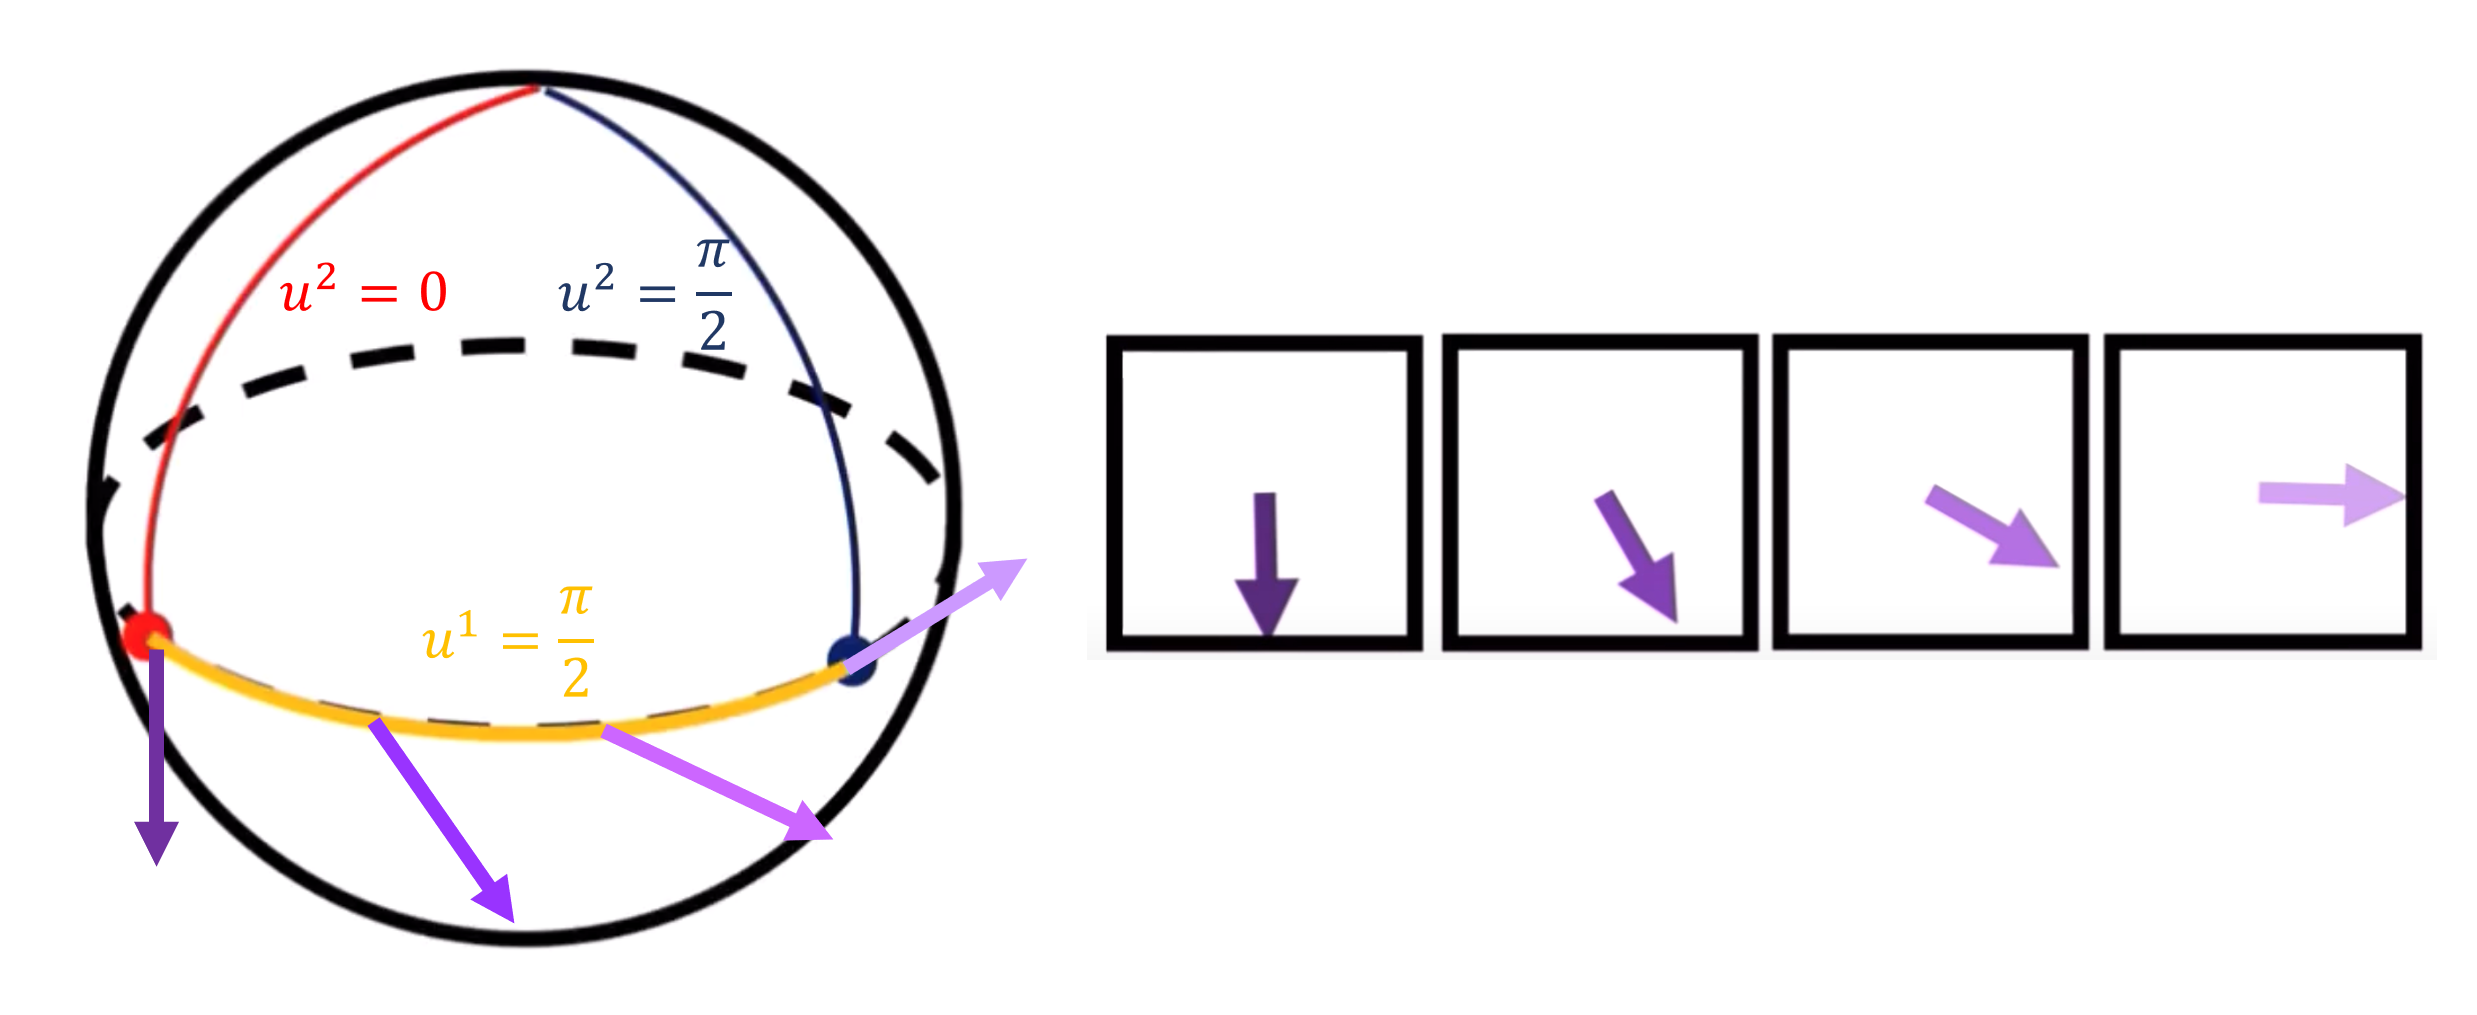
\includegraphics[scale=0.15]{figure/sphere1.png}
   \caption{Exponential and log map}
    \end{figure}
    
    Substitute the $u^1, u^2$ into Eq.(\ref{eq4}), we have
    \begin{align*}
        \nabla_{\Vec{e_2}} \Vec{v}&=\left(\frac{\partial v^1}{\partial u^2}-\frac{1}{2}\sin(2u^1)v^2\right)\Vec{e_1}+\left(\frac{\partial v^2}{\partial u^2}+v^1\cot(u^1)\right)\Vec{e_2}\\
        &=-\sin(u^2)\Vec{e_1}+\cos(u^2)\Vec{e_2},
    \end{align*}
    since $\nabla_{\Vec{e_2}} \Vec{v}\not=\Vec{0}$, which means the rate of change is not completely normal to the tangent space.
    \item The second vector field along the equator is
    \begin{align*}
        \Vec{v}=0\Vec{e_1}+1\Vec{e_2} && \text{where } u^1=\frac{\pi}{2},u^2=\lambda\in[0,\frac{\pi}{2}]
    \end{align*}
    
    \begin{figure}[H]
   \centering
   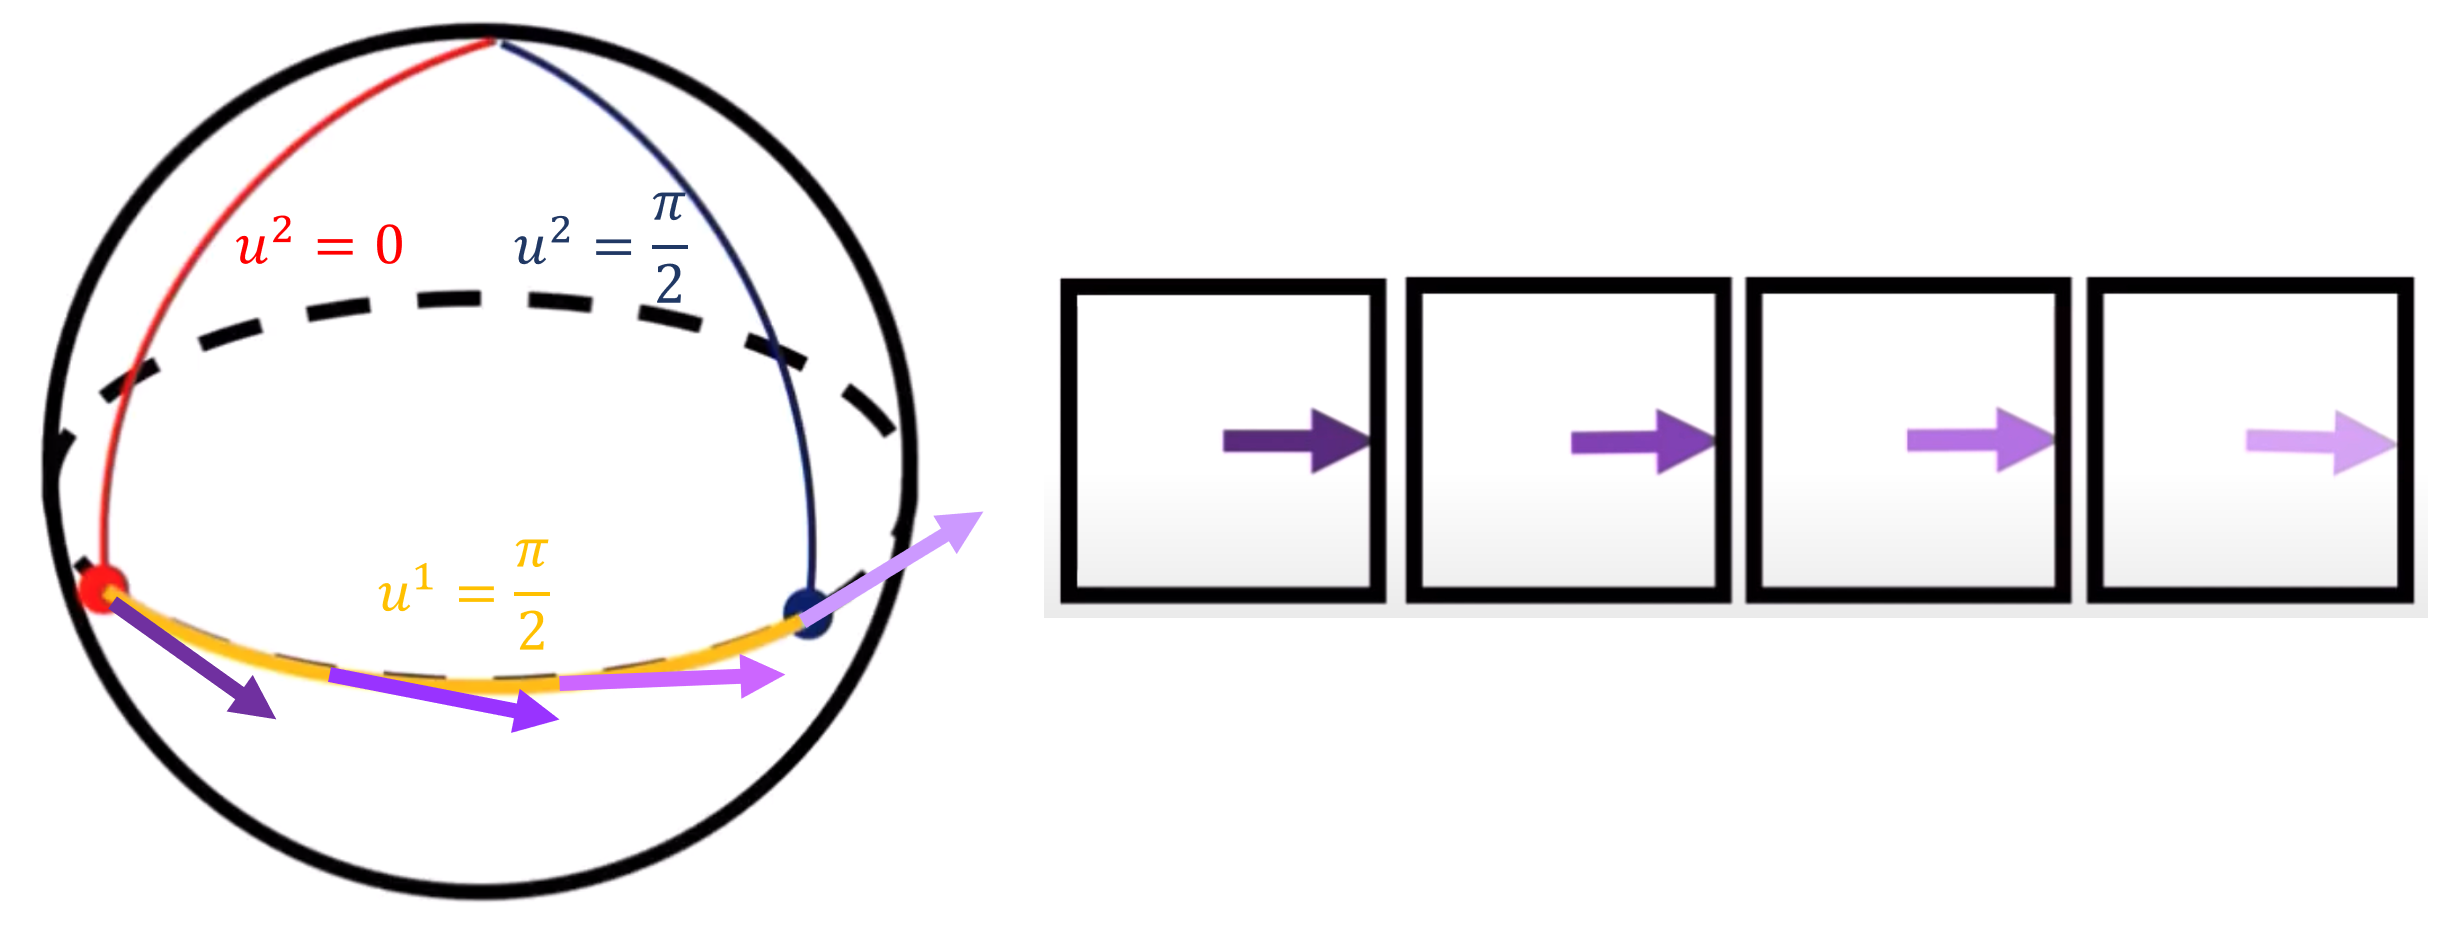
\includegraphics[scale=0.15]{figure/sphere2.png}
   \caption{Exponential and log map}
    \end{figure}
    
    Since the vector field has nothing to do with $u^1,u^2$, we have
    \begin{align*}
        \nabla_{\Vec{e_2}} \Vec{v}&=\left(\frac{\partial v^1}{\partial u^2}-\frac{1}{2}\sin(2u^1)v^2\right)\Vec{e_1}+\left(\frac{\partial v^2}{\partial u^2}+v^1\cot(u^1)\right)\Vec{e_2}\\
        &=(0-0)\Vec{e_1}+(0+0)\Vec{e_2}=\Vec{0},
    \end{align*}
    which means the rate of change doesn't exist in the tangent space. And this is exactly the geodesic which is resulted from parallel transporting a vector along itself.
\end{itemize}
\end{example}

\begin{example}\cite{cd3}
In extrinsic case, we have to subtract the normal component, however, in intrinsic case, such normal component doesn't exist, so we have
\begin{align*}
    \nabla_\frac{\partial}{\partial u^i}\Vec{v}&=\frac{\partial\vec{v}}{\partial u^i}\\
    &=\frac{\partial}{\partial u^i}(v^j\vec{e_j})\\
    &=\frac{\partial v^j}{\partial u^i}\vec{e_j}+v^j\frac{\partial\vec{e_j}}{\partial u^i}\\
    &=\frac{\partial v^k}{\partial u^i}\vec{e_k}+v^j\Gamma^k_{ij}\vec{e_k} && \triangleright  \frac{\partial\vec{e_j}}{\partial u^i}=\Gamma^k_{ij}\vec{e_k}\\
    &=\left(\frac{\partial v^k}{\partial u^i}+v^j\Gamma^k_{ij}\right)\vec{e_k}
\end{align*}

The only difference between the extrinsic and intrinsic cases lies in the calculation of Christoffel symbol. Previously, we derived the christoffel symbol in Eq.(\ref{chrisex}), by inner product between Eq.(\ref{eq2},\ref{eq3},\ref{eq5},\ref{eq6},\ref{eq7}), given the position vector. However, in intrinsic case, there's no longer a position vector, so we have to find another way to derive the Christoffel symbol. And it turns out using the metric:
\begin{align*}
    \frac{\partial}{\partial u^k}g_{ij}&=\frac{\partial}{\partial u^k}(\vec{e_i}\cdot\vec{e_j}) &&\triangleright  g_{ij}=\frac{\partial}{\partial u^i}\cdot\frac{\partial}{\partial u^j}=\vec{e_i}\cdot\vec{e_j}\\
    &=\frac{\partial \vec{e_i}}{\partial u^k}\cdot\vec{e_j}+\vec{e_i}\cdot\frac{\partial\vec{e_j}}{\partial u^k}\\
    &=(\Gamma^l_{ik}\vec{e_l})\cdot\vec{e_j}+\vec{e_i}\cdot(\Gamma^l_{jk}\vec{e_l})\\
    &=\Gamma^l_{ik}(\vec{e_l}\cdot\vec{e_j})+\Gamma^l_{jk}(\vec{e_i}\cdot\vec{e_l})\\
    &=\Gamma^l_{ik}g_{lj}+\Gamma^l_{jk}g_{il}
\end{align*}

Similarly, we can yield other two expressions:
\begin{align*}
    \frac{\partial g_{ij}}{\partial u^k}&=\Gamma^l_{ik}g_{jl}+\Gamma^l_{jk}g_{il}\\
    \frac{\partial g_{ki}}{\partial u^j}&=\Gamma^l_{kj}g_{il}+\Gamma^l_{ij}g_{kl}\\
    \frac{\partial g_{jk}}{\partial u^i}&=\Gamma^l_{ji}g_{kl}+\Gamma^l_{ki}g_{jl}
\end{align*}

Add the two of them up and subtract the left one:
\begin{align*}
    \frac{\partial g_{ij}}{\partial u^k}+\frac{\partial g_{ki}}{\partial u^j}-\frac{\partial g_{jk}}{\partial u^i}
    &=\Gamma^l_{ik}g_jl+\Gamma^l_{jk}g_{il}+\Gamma^l_{kj}g_{il}+\Gamma^l_{ij}g_{kl}-\Gamma^l_{ji}g_{kl}-\Gamma^l_{ki}g_{jl}\\
    &=\Gamma^l_{jk}g_{il}+\Gamma^l_{kj}g_{il}\\
    &=2\Gamma^l_{kj}g_{il}
\end{align*}

Times $g^{im}$ on both sides, we can finally get the intrinsic expression of the Christoffel symbol:
\begin{align*}
    2\Gamma^l_{kj}g_{il}g^{im}&=g^{im}\left(\frac{\partial g_{ij}}{\partial u^k}+\frac{\partial g_{ki}}{\partial u^j}-\frac{\partial g_{jk}}{\partial u^i}\right)\\
    \Gamma^l_{kj}\delta_{l}^{m}&=\frac{1}{2}g^{im}\left(\frac{\partial g_{ij}}{\partial u^k}+\frac{\partial g_{ki}}{\partial u^j}-\frac{\partial g_{jk}}{\partial u^i}\right)\\
    \Gamma^m_{kj}&=\frac{1}{2}g^{im}\left(\frac{\partial g_{ij}}{\partial u^k}+\frac{\partial g_{ki}}{\partial u^j}-\frac{\partial g_{jk}}{\partial u^i}\right)
\end{align*}

The derivation below illustrates the extrinsic and intrinsic expressions of the Christoffel symbols are actually the same:
\begin{align*}
    \frac{\partial g_{ij}}{\partial u^k}+\frac{\partial g_{ki}}{\partial u^j}-\frac{\partial g_{jk}}{\partial u^i}
    &=\frac{\partial\vec{e_i}}{\partial u^k}\cdot\vec{e_j}+\vec{e_i}\cdot\frac{\partial\vec{e_j}}{\partial u^k} && \triangleright  \frac{\partial g_{ij}}{\partial u^k}=\frac{\partial\vec{e_i}}{\partial u^k}\cdot\vec{e_j}+\vec{e_i}\cdot\frac{\partial\vec{e_j}}{\partial u^k}\\
    &+\frac{\partial\vec{e_k}}{\partial u^j}\cdot\vec{e_i}+\vec{e_k}\cdot\frac{\partial\vec{e_j}}{\partial u^i}\\
    &-\frac{\partial\vec{e_j}}{\partial u^i}\cdot\vec{e_k}-\vec{e_j}\cdot\frac{\partial\vec{e_i}}{\partial u^k}\\
    &=2\vec{e_i}\cdot\frac{\partial\vec{e_k}}{\partial u^j} &&\triangleright  \frac{\vec{e_j}}{u^i}=\frac{\vec{e_i}}{u^j}
\end{align*}
    
\begin{align*}
    \Gamma^m_{kj}&=\frac{1}{2}g^{im}\left(\frac{\partial g_{ij}}{\partial u^k}+\frac{\partial g_{ki}}{\partial u^j}-\frac{\partial g_{jk}}{\partial u^i}\right)\\
    &=\frac{1}{2}g^{im}\cdot2\vec{e_i}\cdot\frac{\partial\vec{e_j}}{\partial u^j}\\
    &=\left(\vec{e_i}\cdot\frac{\partial\vec{e_k}}{\partial u^j}\right)g^{mi}
\end{align*}
\end{example}

\begin{definition}
\boxed{\textbf{First fundamental form}} on manifold $M$ is the field which assigns to each $p\in M$ the bilinear map
\begin{align*}
    g_p(v,w)&:T_pM\times T_pM\rightarrow\mathbb{R}\\
    g_p(v,w)&=\langle v,w\rangle
\end{align*}
where $v,w\in T_pM$.
\end{definition}

\begin{definition}
\boxed{\textbf{Second fundamental form}} on manifold $M$ is defined by
\begin{align*}
    h_p(v,w)&:T_pM\times T_pM\rightarrow T_pM^\perp\\
    h_p(v,w)&=(d\Pi(p)v)w=(d\Pi(p)w)v
\end{align*}
where $p\in M$ and $v,w\in T_pM$.
\end{definition}

\begin{definition}
\boxed{\textbf{Riemannian exponential map}} takes the position $p=\gamma(0)\in M$ and velocity $v=\Dot{\gamma}(0)\in T_pM$ as input and returns the point at time 1 along the geodesic with these initial conditions. When $\gamma$ is defined over the interval $[0,1]$, the Riemannian exponential map at $p$ is defined as
\begin{align*}
    \mathrm{Exp}_p(v)&:T_pM\rightarrow M\\
    \mathrm{Exp}_p(v)&=\mathrm{Exp}(p,v)=\gamma(1)
\end{align*}
\end{definition}

\begin{example}
For a Lie group with bi-invariant metric, the Lie group exponential map is the same with the Riemannian exponential map at the identity, that is, for any tangent vector $X\in\mathfrak{g}$, we have
\begin{equation*}
    \mathrm{exp}(X)=\mathrm{Exp}_e(X).
\end{equation*}
For matrix groups, the Lie group exponential map of a matrix $X\in\mathfrak{gl}(n)$ is computed by the formular
\begin{equation*}
    \mathrm{exp}(X)=\sum^\infty_{k=0}\frac{1}{k!}X^k.
\end{equation*}
This series converges absolutely for all $X\in\mathfrak{gl}(n)$
\end{example}

\begin{definition}
\boxed{\textbf{Riemannian log map}} is the inverse of Riemannian exponential map, defined in the neighborhood $\mathrm{Exp}_p(v)$
\begin{align*}
    \mathrm{Log}_p&:M\rightarrow T_pM\\
    \mathrm{Log}_p&(\gamma(1))=v
\end{align*}
\end{definition}

\begin{remark}
The matrix logarithm of $M$ is defined as
\begin{equation*}
    \log(M)=X^{-1}\log(D)X,
\end{equation*}
where $M\in\mathcal{R}^{n\times n}$ is a diagonalizable matrix, $X\in\mathcal{R}^{n\times n}$ and $D\in\mathcal{R}^{n\times n}$ is a diagonal matrix. $\log(D)\in\mathcal{R}^{n\times n}$ is also a diagonal matrix with diagonal elements equals to the logarithm of the corresponding diagonal elements of $D$.
\end{remark}

\begin{remark}
According to the property above, we can also have 
\begin{align*}
    \mathrm{tr}(\log(M))&=\mathrm{tr}(X^{-1}\log(D)X)\\
    &=\mathrm{tr}(XX^{-1}\log(D))\\
    &=\mathrm{tr}(\log(D))
\end{align*}
\end{remark}

\begin{figure}[H]
   \centering
   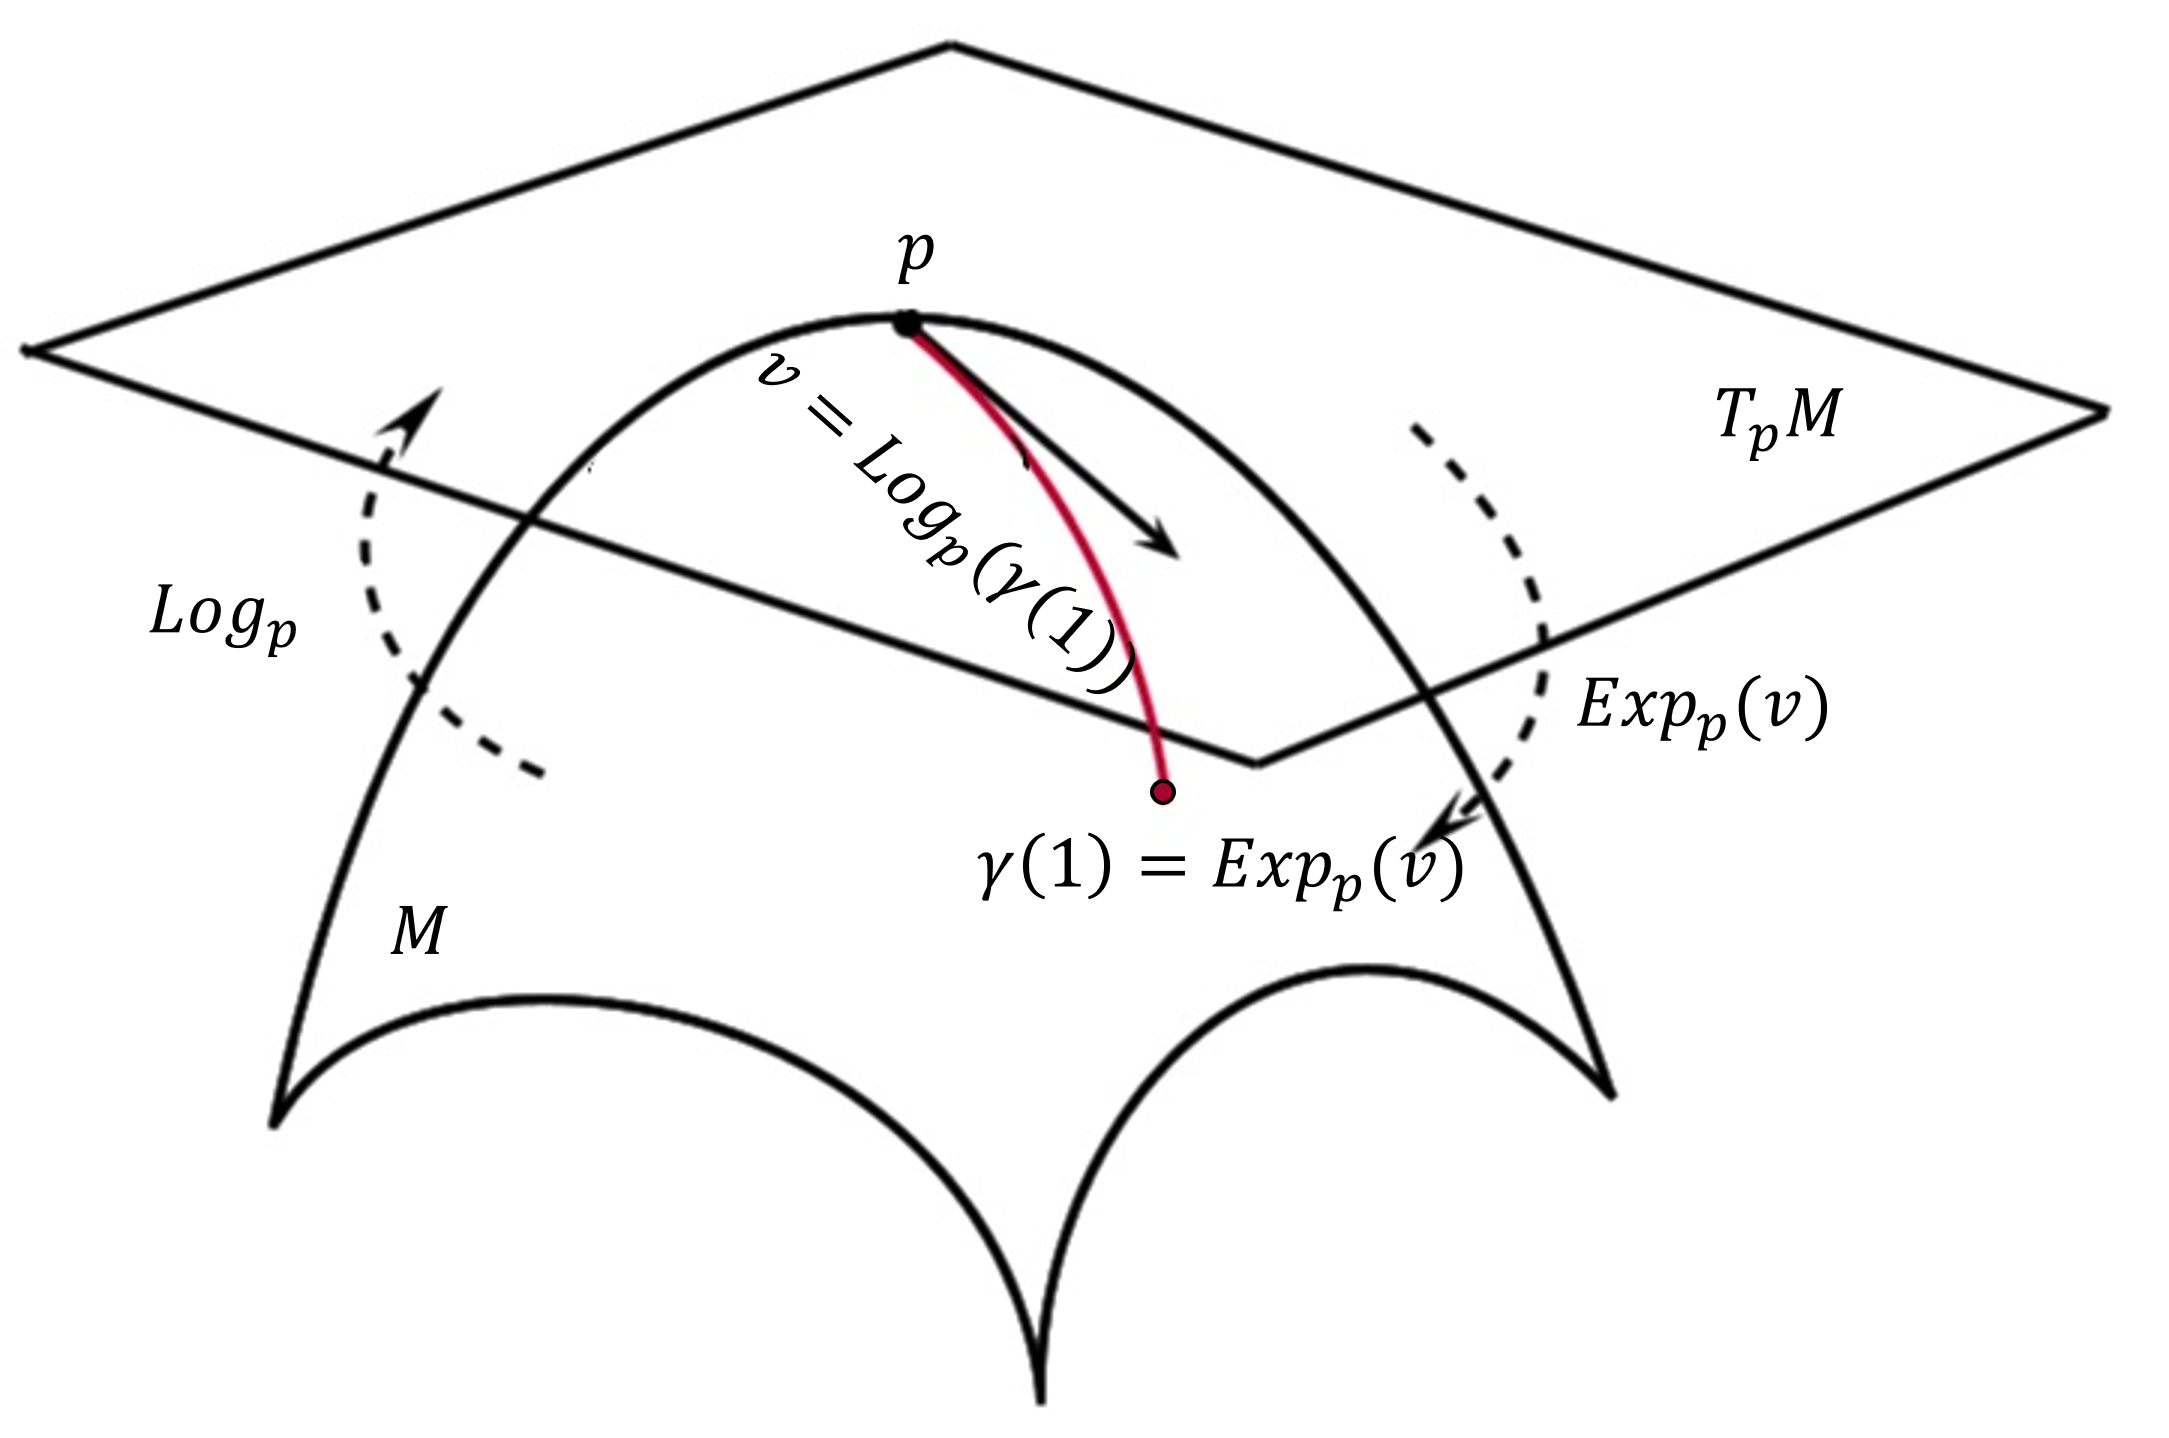
\includegraphics[scale=0.15]{figure/map.png}
   \caption{Exponential and log map}
\end{figure}

\begin{definition}
\boxed{\textbf{Group}} $G$ is a set of elements with a binary operation $\cdot$, such that
\begin{enumerate}
    \item $\forall x,y\in G, x\cdot y\in G$
    \item $\forall x,y\in G, (x\cdot y)\cdot z=x\cdot( y\cdot z)$
    \item $\exists e\in G, \forall x\in G$ satisfy $e\cdot x=x\cdot e=x$, where $e$ is unique
    \item $\forall x\in G, \exists y\in G$ such that $y\cdot x=x\cdot y=e$
\end{enumerate}
\end{definition}

\begin{definition}
\boxed{\textbf{Lie group}} is a smooth manifold equipped with group structures, where the two group operations
\begin{align*}
    &(x,y)\rightarrow x\cdot y:G\times G\rightarrow G &&\text{Multiplication}\\
    &x\rightarrow x^{-1}:G\rightarrow G  &&\text{Inverse}
\end{align*}
are both smooth mappings. In other words, a Lie group adds a smooth manifold structure to a group.
\end{definition}

\begin{definition}
\boxed{\textbf{Orbit}} of a point $p\in M$ is defined as 
\begin{equation*}
    G(p)=\{g\cdot p:g\in G\}
\end{equation*}
\end{definition}

\begin{example}
If $G=SO(2)$, the orbit of point $p$ is a circle.
\end{example}

\begin{definition}
\boxed{\textbf{Lie algebra}} is a \textbf{vector space} $\mathfrak{g}$ together with an operation called Lie bracket $[\cdot,\cdot]$, a alternating bilinear map $\mathfrak{g}\times\mathfrak{g}\rightarrow\mathfrak{g}$. $\forall x,y,z\in\mathfrak{g}\text{ and }a,b\in\mathbb{R}$, the following axioms are satisfied:
\begin{enumerate}
    \item Linearity: $[ax+by,z]=a[x,z]+b[y,z]$
    \item Anticommutativity: $[x,y]=-[y,x]=x\cdot y-y\cdot x$
    \item Jacobi identity: $[x,[y,z]]+[z,[x,y]]+[y,[z,x]]=0$
\end{enumerate}
\end{definition} 

\begin{definition}
\boxed{\textbf{Lie derivative of vector fields}}$[X, Y]$ is the derivative of $Y$ along the flow generated by $X$, and is sometimes denoted $\mathcal {L}_XY$ (``Lie derivative of Y along X''). This generalizes to the Lie derivative of any tensor field along the flow generated by $X$.
\begin{equation*}
    [X,Y](f)=X(Y(f))-Y(X(f))\;\;{\text{  for all }}f\in C^{\infty }(M).
\end{equation*}
\end{definition}

\begin{remark}
Coordinate lines are just flow curves along the basis vector. Coordinate flow curves always close, which means Lie bracket of basis vectors always has to be zero vector.
\begin{figure}[H]
   \centering
   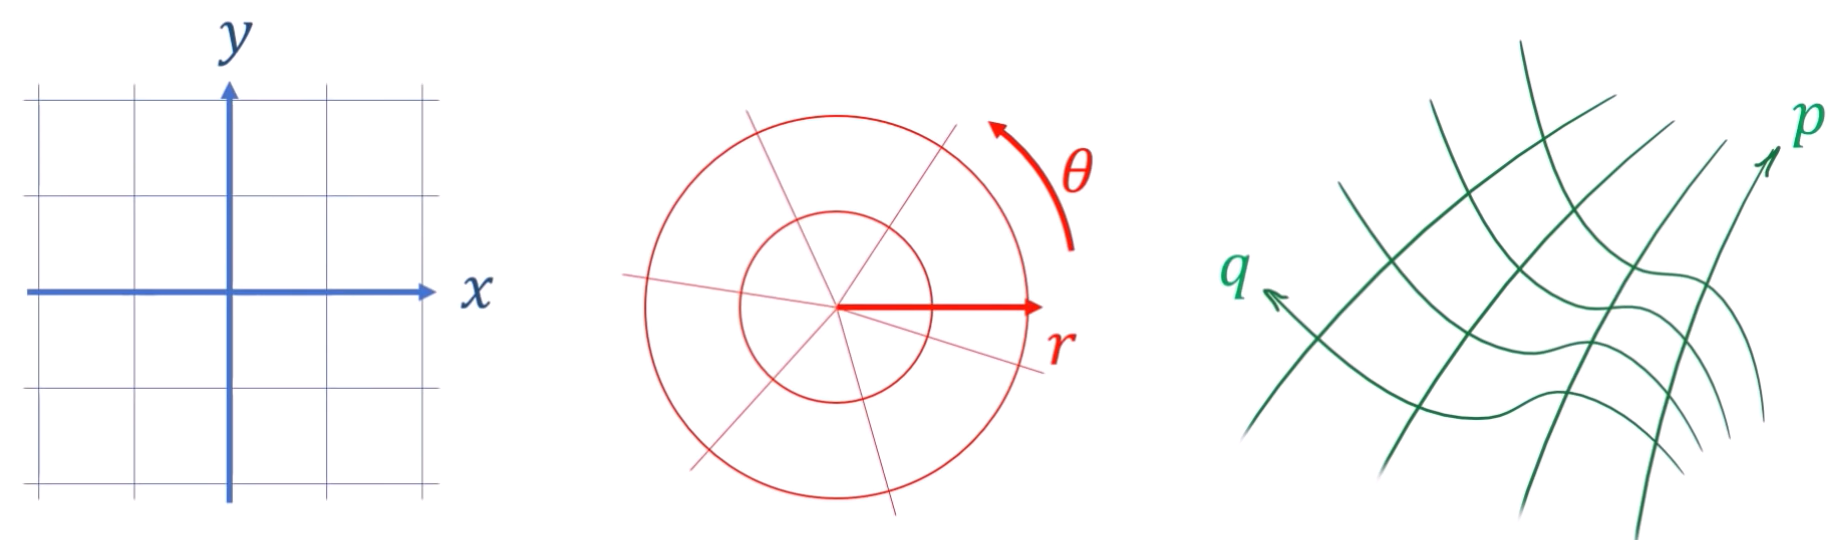
\includegraphics[scale=0.2]{figure/coordinatelines.png}
   \caption{Coordinate lines}
\end{figure}
Lie bracket(commutator) measures how much vector field flow curves fail to close.
\end{remark}

\begin{example}
The example below shows how to calculate the flow curve, given the flow field.
\begin{figure}[H]
   \centering
   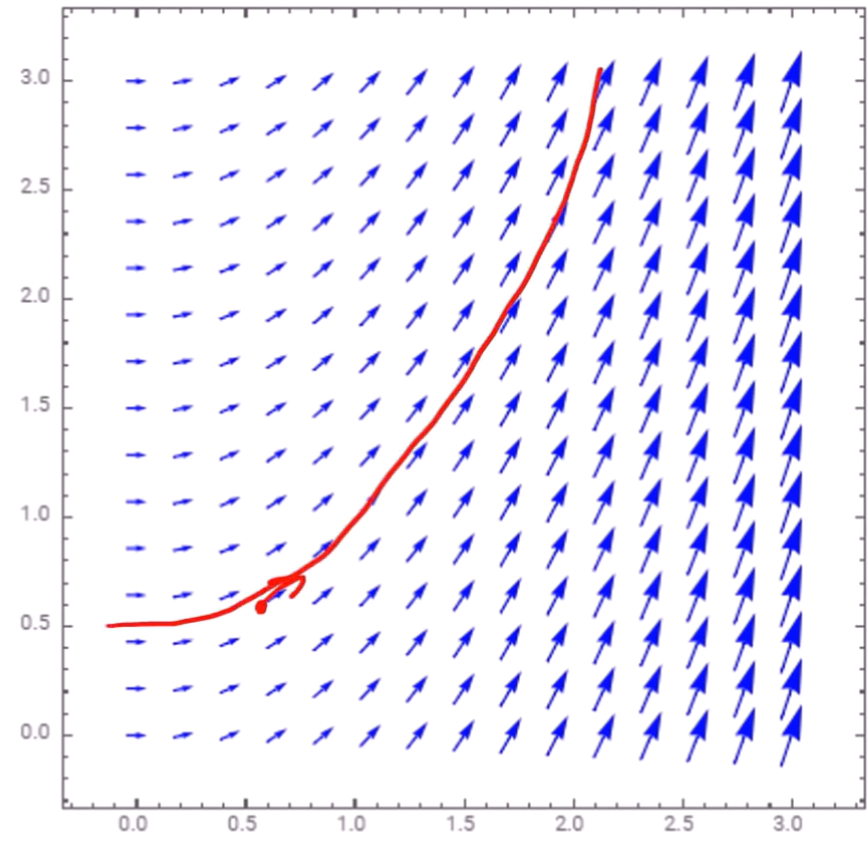
\includegraphics[scale=0.2]{figure/flowfield.png}
   \caption{Flow field}
\end{figure}
Vector arrows tell you velocity at each point:
\begin{equation*}
    \Vec{w}=1\Vec{e_x}+x\Vec{e_y}.
\end{equation*}

To express the vector in the way of position vector $\vec R$, we have
\begin{align*}
    \Vec{w}=\frac{d\Vec{R}}{d\lambda}&=\frac{dx}{d\lambda}\frac{\partial\Vec{R}}{\partial x}+\frac{dy}{d\lambda}\frac{\partial\Vec{R}}{\partial y}\\
    &=\frac{dx}{d\lambda}\Vec{e_x}+\frac{dy}{d\lambda}\Vec{e_y}
\end{align*}

Associating the two expressions above, we can yield the respective expressions of $x,y$.
\begin{align*}
    \frac{dx}{d\lambda}&=1\rightarrow x=\lambda+c_1\\
    \frac{dy}{d\lambda}&=x=\lambda+c_1\rightarrow y=\frac{1}{2}\lambda^2+c_1\lambda+c_2
\end{align*}

Assuming $c_1=c_2=0$, this can be a possible flow curve
\begin{equation*}
    x(\lambda)=\lambda, y(\lambda)=\frac{1}{2}\lambda^2,
\end{equation*}
which is tangent to all vectors in a vector field.
\end{example}

\begin{example}
The Lie bracket of the vector field is defined below:
\begin{equation*}
    [\Vec{u},\Vec{v}]=\underbrace{\Vec{u}(\Vec{v})}_{\text{derivative of }\Vec{v}\text{ in the direction of }\vec{u}}-\Vec{v}(\Vec{u})
\end{equation*}

We separate the flow field in the example above into two fields
\begin{figure}[H]
   \centering
   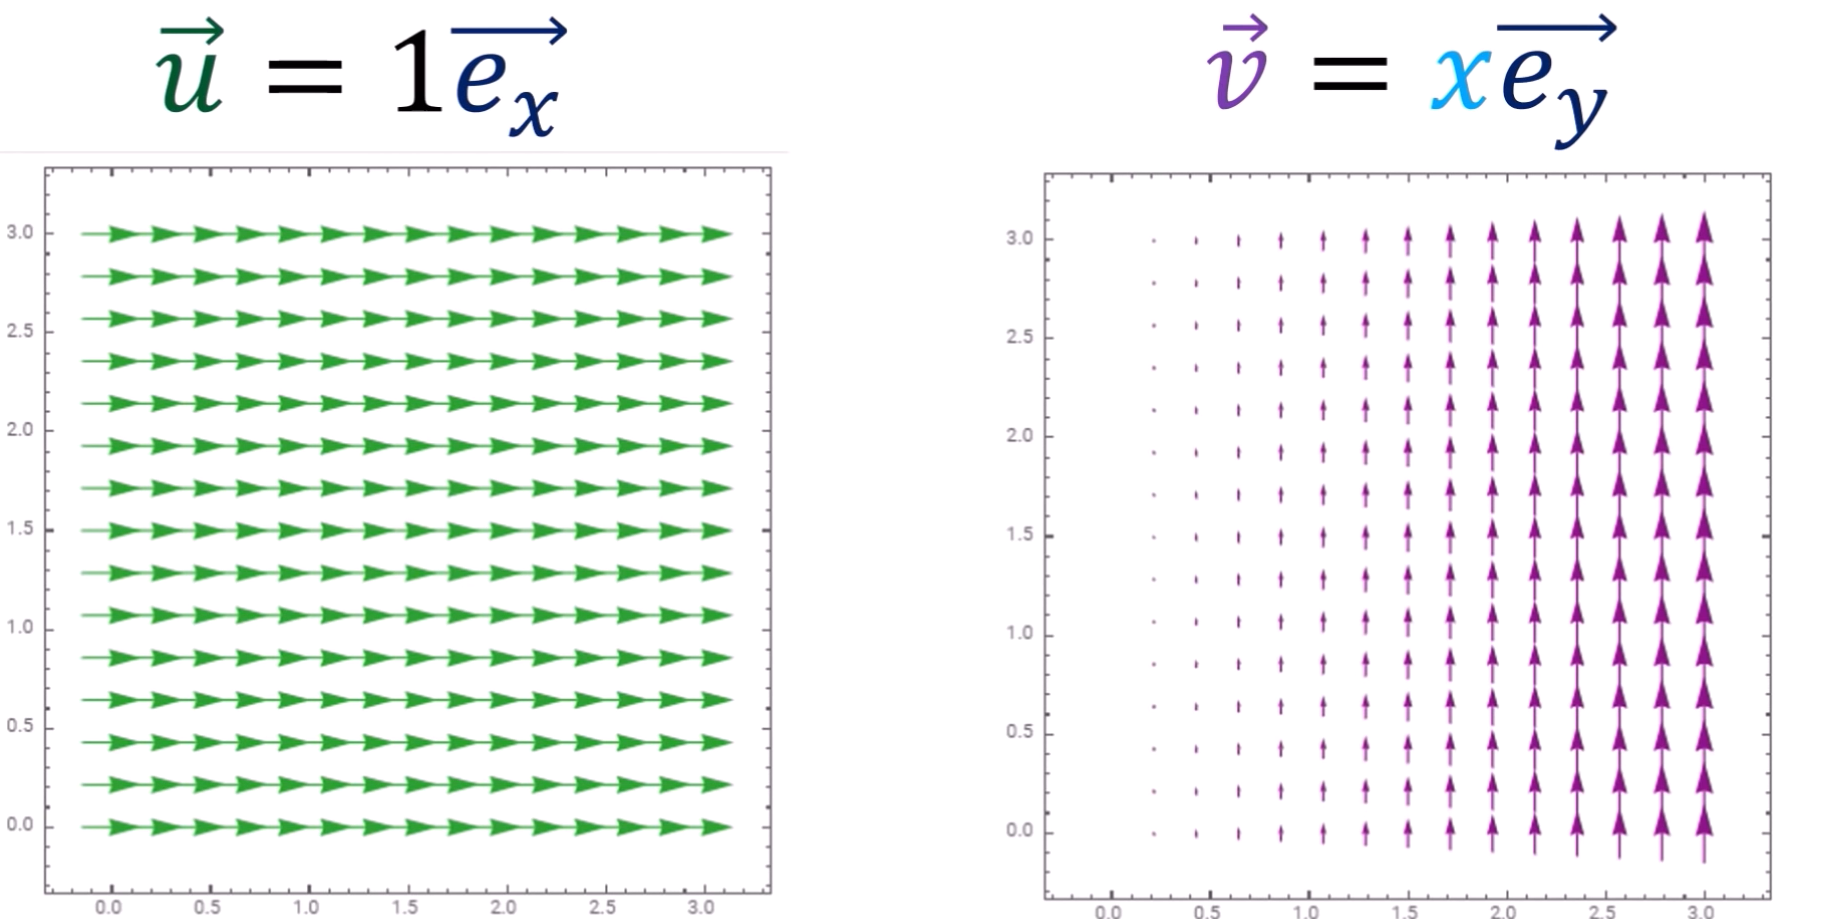
\includegraphics[scale=0.2]{figure/liebracket.png}
   \caption{Two vector fields}
\end{figure}

Derivative of $\Vec{u}$ in the direction of $\vec{v}$ is shown below
\begin{align*}
    \Vec{v}(\Vec{u})&=v^i\Vec{e_i}(u^j\Vec{e_j})\\
    &=v^i\partial_i(u^j\partial_j)\\
    &=v^i[(\partial_iu^j)\partial_j+u^j(\partial_i\partial_j)]&&\triangleright\text{product rule}\\
    &=v^i(\partial_iu^j)\partial_j+v^iu^j(\partial_i\partial_j)\\
    &=v^y(\partial_yu^x)\partial_x+v^yu^x(\partial_y\partial_x)\\
    &=x(\partial_y1)\partial_x+x\cdot1(\partial_y\partial_x)\\
    &=x(\partial_y\partial_x)\\
    &=x(\partial_y\Vec{e_x})\\
    &=x\frac{\Vec{e_x}}{\partial_y}\\
    &=\vec0
\end{align*}

Derivative of $\Vec{v}$ in the direction of $\vec{u}$ is shown below
\begin{align*}
    \Vec{u}(\Vec{v})&=u^i\Vec{e_i}(v^j\Vec{e_j})\\
    &=u^i\partial_i(v^j\partial_j)\\
    &=u^i[(\partial_iv^j)\partial_j+v^j(\partial_i\partial_j)]&&\triangleright\text{product rule}\\
    &=u^i(\partial_iv^j)\partial_j+u^iv^j(\partial_i\partial_j)\\
    &=u^x(\partial_yv^y)\partial_y+u^xv^y(\partial_x\partial_y)\\
    &=1(\partial_xx)\partial_y+1\cdot x(\partial_x\partial_y)\\
    &=\partial_y+x(\partial_y\partial_x)\\
    &=\partial_y+x(\partial_y\Vec{e_x})\\
    &=\partial_y+x\frac{\Vec{e_x}}{\partial_y}\\
    &=\partial_y\\
    &=\Vec{e_y}
\end{align*}

\begin{equation*}
    [\Vec{u},\Vec{v}]=\Vec{u}(\Vec{v})-\Vec{v}(\Vec{u})=\Vec{e_y}-\vec0=\Vec{e_y}
\end{equation*}

These four lines don't give us a closed rectangle. Lie bracket is defined like this to computes the difference between these two derivatives. $\Vec{e_y}$ is the separation vector.
\begin{figure}[H]
   \centering
   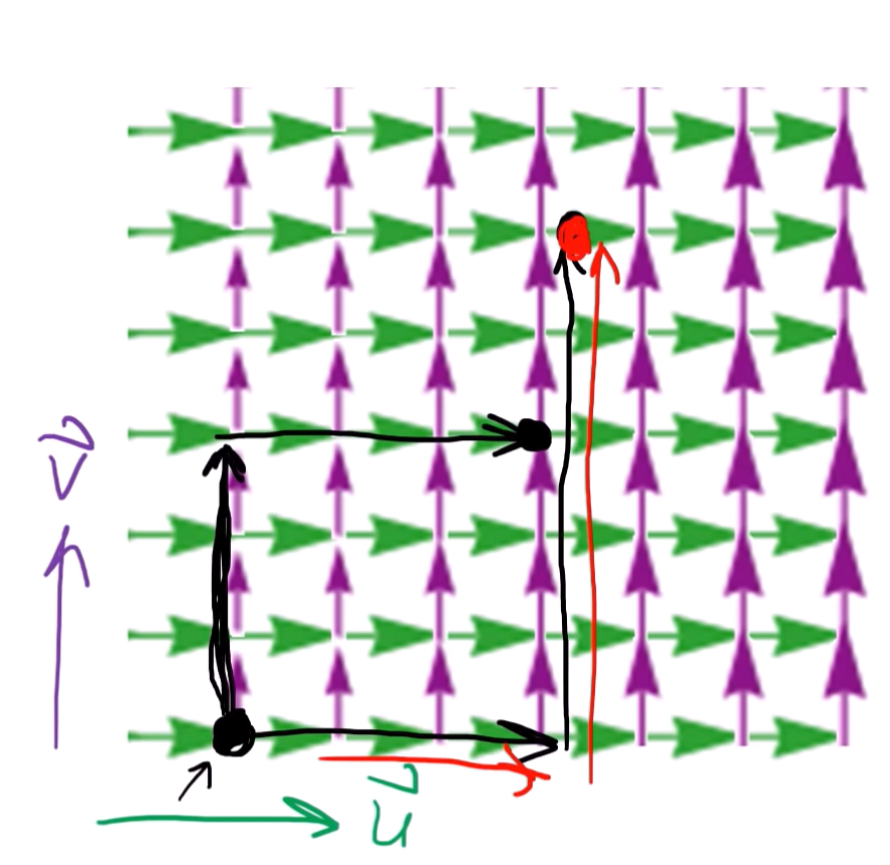
\includegraphics[scale=0.2]{figure/seperation vector.png}
   \caption{Separation vector}
\end{figure}
\end{example}

\begin{definition}
\boxed{\textbf{Lie derivative of tensor fields $T$}} w.r.t. smooth vector field $X$ is defined by
\begin{equation*}
    (\mathcal{L}_XT)_p=\frac{d}{dt}\bigg\rvert_{t=0}(\phi^*_tT)_p=\lim_{t\rightarrow0}\frac{\phi^*_t(T_{\phi_t(p)})-T_p}{t},
\end{equation*}
where $X$ is on smooth manifold $M$, $T$ is the covariant tensor field on $M$ and let $\phi_t(p)=\phi(t,p)$ be a diffeomorphism parameterized by point $p$ and ``time'' $t$. $X$ is induced by $\phi$
\end{definition}

\begin{remark}
Intuitively, if you have a tensor field $T$ and a vector field $X$, then $\mathcal{L}_XT$ is the infinitesimal change you would see when you flow $T$ using the vector field $-X$, which is the same thing as the infinitesimal change you would see in $T$ if you flowed along the vector field $X$.
\end{remark}

\begin{definition}\label{def:isometry}
\boxed{\textbf{Isometry}} $\phi:M\rightarrow N$ is a function which preserves distance between manifold $M$ and $N$. $\forall x\in M$, it has
\begin{enumerate}
    \item The derivative of $\phi$ at $x$ is an isomorphism of tangent space $D\phi_x:T_xM\rightarrow T_{\phi_x}N$
    \item $\forall v,w \in T_xM$, the Riemannian metric preserves as $\langle v,w\rangle=\langle D\phi_x\cdot v,D\phi_x\cdot w\rangle$
\end{enumerate}
\end{definition}

\begin{example}\cite{stanford3}
If $S$ and $S'$ are surfaces with metric $g$ and $g'$, then the surfaces are isometric if there exists $\phi:S\rightarrow S'$ such that for all tangent vector $X_p,Y_p\in T_pS$ and all $p\in S$, we have
\begin{equation*}
    \langle X_p,Y_p\rangle_g=\langle D\phi\cdot X_p,D\phi\cdot Y_p\rangle_{g'}
\end{equation*}
Notice that $D\phi$ is the Jacobian matrix pushes forward tangent vectors from $T_pS$ to $T_{\phi(p)}S'$. We can understand an isometry as preserving the intrinsic geometry at corresponding points.
\end{example}

\begin{definition}
\boxed{\textbf{Isometry group}} $G$ is group of $M$ such that $\forall p,q\in M, g\in G, d(p,q)=d(g\cdot p,g\cdot q)$ holds.
\end{definition}

\begin{definition}
\boxed{\textbf{Conformality}} $\phi:S_1\rightarrow S_2$ is a function that for all $X,Y\in T_pM$, there exists a function $u:M\rightarrow\mathbb{R}$ such that
\begin{equation*}
    e^{2u(p)}\langle X,Y\rangle_{g_1}=\langle D\phi_p\cdot X,D\phi_p\cdot Y\rangle_{g_2},
\end{equation*}
where $g_1,g_2$ are the metrics of $S_1, S_2$ at points $p,\phi(p)$.
\end{definition}

\begin{remark}\cite{stanford4}
Compared to isometries that preserve both lengths and angles, conformality is a weaker condition that preserves only angles. Conformality is very flexible, in fact, all surfaces are locally conformal to the Euclidean metric.
\end{remark}

\begin{definition}
\boxed{\textbf{Isotropy subgroup}} of $p$ is defined as $G_p=\{g\in G|g\cdot p=p\}$. In other words, $G_p$ is the subgroup of $G$ which leaves $p$ fixed.
\end{definition}

\begin{definition}
\boxed{\textbf{Symmetric space}} is a connected Riemannian manifold $M$ such that $\forall p\in M$, there is an involutive isometry $\phi_p:M\rightarrow M$ that has $p$ as an isolated fixed point. A point $x\in X$ is called a fixed point of $\phi$ if $\phi(x)=x$.
\end{definition}

\newpage
\section{Adjoint Representation}
\begin{definition}
\boxed{\textbf{Automorphism group}}\cite{singh} $\Psi:G\rightarrow G$ is defined as
\begin{equation*}
    \Psi_g(h)=ghg^{-1}
\end{equation*}
given $\forall g,h\in G$.
\end{definition}

\begin{definition}
\boxed{\textbf{Inner automorphism group}} $\mathrm{Inn}(G)$ is the collection of all inner automorphisms of the form $\Psi_g,\forall g\in G$. $\mathrm{Inn}(G)$ is a Lie group and commutative.
\end{definition}

\begin{definition}
\boxed{\textbf{Dual pairing}} $(m,v)$, where $m\in V^*$, the dual space to $V$, and $v\in V$
\end{definition}

\begin{definition}
\boxed{\textbf{Adjoint action $\mathrm{Ad}_g$}} is the derivative of $\Psi_g(h)$ with respect to $h$ at the identity, which is
\begin{align*}
    \mathrm{Ad}_g&:G\times\mathfrak{g}\rightarrow\mathfrak{g}\\
    \mathrm{Ad}_g&=d(\Psi_g)_e
\end{align*}
\end{definition}

\begin{itemize}
    \item For matrix group, $\mathrm{Ad}_g$ is derived as
    \begin{align*}
        \mathrm{Ad}_gw&=\frac{\partial}{\partial\xi}\Psi_g(w)\\
        &=\frac{\partial}{\partial\xi}\Psi_g(h_\xi|_{\xi=0})\\
        &=\frac{\partial}{\partial\xi}\left(g(h_\xi|_{\xi=0})g^{-1}\right)\\
        &=g\left(\frac{\partial}{\partial\xi}h_\xi|_{\xi=0}\right)g^{-1}\\
        &=gwg^{-1}
    \end{align*}
    where $h_\xi$ denotes the variation of $h$ by $\xi$ such that $h_0=e$ and $\frac{\partial}{\partial\xi}h_\xi|_{\xi=0}=w$ for $\Psi_g(h_\xi)=gh_\xi g^{-1}$.
    
    \item For conjugation of operators under dual pairing, using $\mathrm{Ad}_gw=gwg^{-1}$, we have
    \begin{align*}
        (m,\mathrm{Ad}_gw)&=(m,gwg^{-1})\\
        &=(g^Tm,wg^{-1})\\
        &=(g^Tmg^{-T},w)\\
        \mathrm{Ad}^*_gm&=g^Tmg^{-T},
    \end{align*}
    as if $A$ is a linear operator from $V$ to $V$, its conjugate $A^*:V^*\rightarrow V^*$ is defined by $(A^*m,v)=(m,Av)$. For detail, see  \cite{singh}.
    
    \item For $\mathrm{Diff}(\Omega)$, $\mathrm{Ad}_\phi$ is derived as
    \begin{align*}
        \mathrm{Ad}_\phi w&=\frac{\partial}{\partial\xi}(\Psi_\phi h_\xi)|_{\xi=0}\\
        &=\frac{\partial}{\partial\xi}(\phi\circ h_\xi\circ\phi^{-1})|_{\xi=0}\\
        &=D\phi|_{h_\xi\circ\phi^{-1}}w|_{\phi^{-1}}\\
        &=(D\phi\circ\phi^{-1})w\circ\phi^{-1}
    \end{align*}
    where $h_\xi$ denotes the variation of $h$ by $\xi$ such that $h_0=\mathrm{Id}$ and $\frac{\partial}{\partial\xi}h_\xi|_{\xi=0}=w$ for $\Psi_\phi(h_\xi)=\phi\circ h_\xi \circ\phi^{-1}$.
\end{itemize}

\begin{example}
Adjoint of the gradient is the negative divergence:
\begin{equation*}
    \langle\nabla f,g\rangle=-\langle f,\mathrm{div}g\rangle
\end{equation*}
\end{example}

\begin{definition}
\boxed{\textbf{Infinitesimal adjoint action $\mathrm{ad}$}} is the derivative of the adjoint map $\mathrm{Ad}$ with respect to $g$ at identity, which is
\begin{align*}
    \mathrm{ad}&:\mathfrak{g}\times\mathfrak{g}\rightarrow\mathfrak{g}\\
    \mathrm{ad}&=d(\mathrm{Ad}_g)_e
\end{align*}
\end{definition}

\begin{itemize}
    \item For matrix group, $\mathrm{ad}_g$ is derived as
    \begin{align*}
        \mathrm{ad}_vw&=\frac{\partial}{\partial\xi}\mathrm{Ad}_{g_\xi}w|_{\xi=0}\\
        &=\frac{\partial}{\partial\xi}(g_\xi wg_\xi^{-1})|_{\xi=0}\\
        &=\left(\frac{\partial}{\partial\xi}g_\xi wg_\xi^{-1}\right)\bigg\rvert_{\xi=0}+\left(g_\xi w\frac{\partial}{\partial\xi}g_\xi^{-1}\right)\bigg\rvert_{\xi=0}\\
        &=vw-\left(g_\xi wg_\xi^{-1}\frac{\partial}{\partial\xi}g_\xi g_\xi^{-1}\right)\bigg\rvert_{\xi=0}\\
        &=vw-wv
    \end{align*}
    where $g_\xi$ is the variation of $g$ by $\xi$ with $g_0=e$ and $\frac{\partial}{\partial \xi}g_\xi|_{\xi=0}=v$ for $\mathrm{Ad}_{g_\xi}w=g_\xi w g^{-1}_\xi$.
    
    \item For conjugation of operators under dual pairing, using $\mathrm{ad}_vw=vw-wv$, we have
    \begin{align*}
        (m,\mathrm{ad}_vw)&=(m,vw-wv)\\
        &=(m,vw)-(m,wv)\\
        &=(v^Tm,w)-(mv^T,w)\\
        &=(v^Tm-mv^T,w)\\
        \mathrm{ad}^*_vm&=v^Tm-mv^T,
    \end{align*}
    as if $A$ is a linear operator from $V$ to $V$, its conjugate $A^*:V^*\rightarrow V^*$ is defined by $(A^*m,v)=(m,Av)$. For detail, see  \cite{singh}.
    
    \item For $\mathrm{Diff}(\Omega)$, $\mathrm{ad}_v$ is derived as
    \begin{align*}
        \mathrm{ad}_vw&=\frac{\partial}{\partial\xi}((D\phi_\xi\circ\phi^{-1}_\xi)w\circ\phi^{-1}_\xi)|_{\xi=0}\\
        &=\frac{\partial}{\partial\xi}((D\phi_\xi\circ\phi^{-1}_\xi))|_{\xi=0}w+D\mathrm{Id}\frac{\partial}{\partial\xi}(w\circ\phi^{-1}_\xi)|_{\xi=0}\\
        &=\left((\frac{\partial}{\partial\xi}D\phi_\xi|{\phi^{-1}_\xi}+DD\phi_\xi|_{\xi=0}D\phi^{-1}_\xi)w\circ\phi^{-1}_\xi+Dv|_{\phi^{-1}_\xi}\frac{\partial\phi^{-1}_\xi}{\partial\xi}\right)\bigg\rvert_{\xi=0}\\
        &=(Dv+0)w-Dwv\\
        &=Dvw-Dwv
    \end{align*}
    where $\phi_\xi$ is the variation of $\phi$ by $\xi$ with $\phi_0=e$ and $\frac{\partial}{\partial \xi}\phi_\xi|_{\xi=0}=v$ for $\mathrm{Ad}_{\phi}w=(D\phi\circ\phi^{-1})w\circ\phi^{-1}$.
\end{itemize}


\begin{definition}
\boxed{\textbf{Left/Right multiplication}} is a diffeomorphism such that
\begin{align*}
    &L_y:x\rightarrow y\cdot x & \text{Left Multiplication}\\
    &R_y:x\rightarrow x\cdot y & \text{Right Multiplication}
\end{align*}
where $y\in G$, $G$ is a Lie group.
\end{definition}

\begin{definition}
\boxed{\textbf{Left/Right-invariant}} means $\forall y\in G$, we have $L_{y*}X=X \text{ or } R_{y*}X=X$.
\end{definition}

\begin{example}
The metric $G^I$ has the property of right-invariance: if $U,V\in T_\phi\mathrm{Diff}(M)$ then
\begin{align*}
    G^I_\phi(U,V)=G^I_{\phi\circ\psi}(U\circ\psi,V\circ\psi) && \forall\psi\in\mathrm{Diff}(M)
\end{align*}
\end{example}

\begin{definition}
\boxed{\textbf{Inertia operator}} $L:\mathfrak{g}\rightarrow\mathfrak{g}^*$ is defined by
\begin{equation*}
    \langle v,w\rangle=(Lv,w), \forall v,w\in\mathfrak{g}
\end{equation*}
$L$ must be invertible and
\begin{equation*}
    (Lv,w)=(Lw,v), \forall v,w\in\mathfrak{g}
\end{equation*}
in order to satisfy the properties of a well-formed Riemannian metric.
\end{definition}

\begin{definition}
A linear operator $f:\mathfrak{g}\rightarrow\mathfrak{g}$ is \boxed{\textbf{transposed}} with respect to the inner product defined by $L$, using the formula
\begin{equation*}
    \langle f^\dagger v,w\rangle=\langle v,fw\rangle, \forall v,w\in\mathfrak{g}
\end{equation*}
We use this to define the adjoint-transpose action $\mathrm{Ad}^\dagger:G\times\mathfrak{g}\rightarrow\mathfrak{g}$ via the transpose of $\mathrm{Ad}_g$ and the infinitesimal adjoint-transpose $\mathrm{ad}^\dagger:\mathfrak{g}\times\mathfrak{g}\rightarrow\mathfrak{g}$ via the transpose of $\mathrm{ad}_v$
\end{definition}

\newpage
\section{Diffeomorphism}
\begin{definition}
\boxed{\textbf{Information metric}} $G^I$ is defined by
\begin{equation*}
    G^I_\phi(U,V)=-\int_M\langle\Delta u,v\rangle_g \mathrm{vol}+\lambda\sum^k_{i=1}\left(\int_M\langle u,\xi_i\rangle_g \mathrm{vol}\cdot\int_M\langle v,\xi_i\rangle_g \mathrm{vol}\right),
\end{equation*}
where $U=u\circ\phi, V=v\circ\phi, \lambda>0, \Delta$ is the Laplace-de Rham operator lifted to vector fields, and $\xi_1,\cdots,\xi_k$ is an orthonormal basis of the harmonic 1-form on $M$.
\end{definition}

\begin{definition}
\boxed{\textbf{Fisher-Rao metric}} is the Riemannian metric on $\mathrm{Dens}(M)$ given by
\begin{equation*}
    G^F_\mu(\alpha,\beta)=\frac{1}{4}\int_M\frac{\alpha}{\mu}\cdot\frac{\beta}{\mu}\mu,
\end{equation*}
for tangent vectors $\alpha,\beta\in T_\mu\mathrm{Dens}(M)$. It can be interpreted as the Hessian of relative entropy, or information divergence.
\end{definition}

\begin{definition}
The background metric $g$ on manifold $M$ is called \boxed{\textbf{compatible with}} $\mu$ if $\mathrm{vol}_g=\mu$, for $\mu\in\mathrm{Dens}(M)$.
\end{definition}

\begin{definition}
\boxed{\textbf{Set of vector space isomorphisms}} $\mathcal{L}_{iso}$ is defined by
\begin{equation*}
    \mathcal{L}_{iso}(\mathbb{R}^m,V)=\{e:\mathbb{R}^m\rightarrow V|e \text{ is a vector space isomorphism}\}.
\end{equation*}
\end{definition}

\begin{definition}
\boxed{\textbf{Frame}} of $m$-dimension real vector space $V$ is the basis $e_1,\cdots,e_m$ of $V$.
\end{definition}

\begin{definition}
\boxed{\textbf{Frame bundle}} $\mathcal{F}$ of a smooth $m$-dimensional submanifold $M$ is defined by
\begin{equation*}
    \mathcal{F}(M)=\{(p,e)|p\in M,e\in\mathcal{F}(M)_p\},
\end{equation*}
where $\mathcal{F}(M)_p=\mathcal{L}_{iso}(\mathbb{R}^m,T_pM)$ is the space of frames of tangent space at $p$.
\end{definition}

\begin{definition}
A smooth curve $\beta:\mathbb{R}\rightarrow\mathcal{F}(M)$ is called a \boxed{\textbf{lift}} of smooth curve $\gamma:\mathbb{R}\rightarrow M$ if \cite{robbin}
\begin{equation*}
    \pi\circ\beta=\gamma.
\end{equation*}
\end{definition}

\begin{example}
The general linear group $GL(m,\mathbb{R})$ acts on this space by composition on the right via
\begin{equation*}
    GL(m)\times\mathcal{L}_{iso}(\mathbb{R}^m,V)\rightarrow\mathcal{L}_{iso}(\mathbb{R}^m,V):(a,e)\rightarrow a^*e=e\circ a
\end{equation*}
\end{example}

\begin{definition}
A curve $\beta(t)=(\gamma(t),e(t))\in\mathcal{F}(M)$ is called \boxed{\textbf{horizontal lift}} of $\gamma$ if the vector field $X(t)=e(t)\xi$ along $\gamma$ is parallel for every $\xi\in\mathbb{R}^m$. Thus a horizontal lift of $\gamma$ has the form
\begin{equation*}
    \beta(t)=(\gamma(t),\Phi_\gamma(t,0)e)
\end{equation*}
for some $e\in\mathcal{L}_{iso}(\mathbb{R}^m,T_{\gamma(0)}M)$.
\end{definition}

\begin{definition}
Suppose $\phi:M\rightarrow N$ is a differential map from $M$ to $N$, $\gamma:(-\epsilon,\epsilon)\rightarrow M$ is a curve on $M$, $\gamma(0)=p,\gamma'(0)=v\in T_pM$, then $\phi\circ\gamma$ is a curve on $N$, $\phi\circ\gamma(0)=\phi(p)$, we define the tangent vector
\begin{equation*}
    \phi_*(v)=(\phi\circ\gamma)'(0)\in T_{\phi(p)}N,
\end{equation*}
as the \boxed{\textbf{pushforward}} tangent vector of $v$ induced by $\phi$.
\end{definition}

\begin{definition}
\boxed{\textbf{Pullback and pushforward}} are defined as below
\begin{align*}
    \text{Pullback(right action):  }\varphi^*\rho&=|D\varphi|\rho(\varphi(\cdot))\\
    &=|D\varphi|\rho\circ\varphi\\
    \text{Pushforward(left action):  }\varphi_*\rho&=(\varphi^{-1})^*\rho\\
    &=|D\varphi^{-1}|\rho(\varphi^{-1}(\cdot))\\
    &=|D\varphi^{-1}|\rho\circ\varphi^{-1}
\end{align*}
where $(\varphi,\rho)\in\mathrm{Diff}(M)\times\mathrm{Dens}(M)$.
\end{definition}

\begin{remark}
Given a $\phi$, there can be two effects or two directions of the $\phi$. The pullback is the one from distorted to checkered, while the pushforward is the one from checkered to distorted, which is more intuitive.
\end{remark}

\begin{figure}[H]
\centering
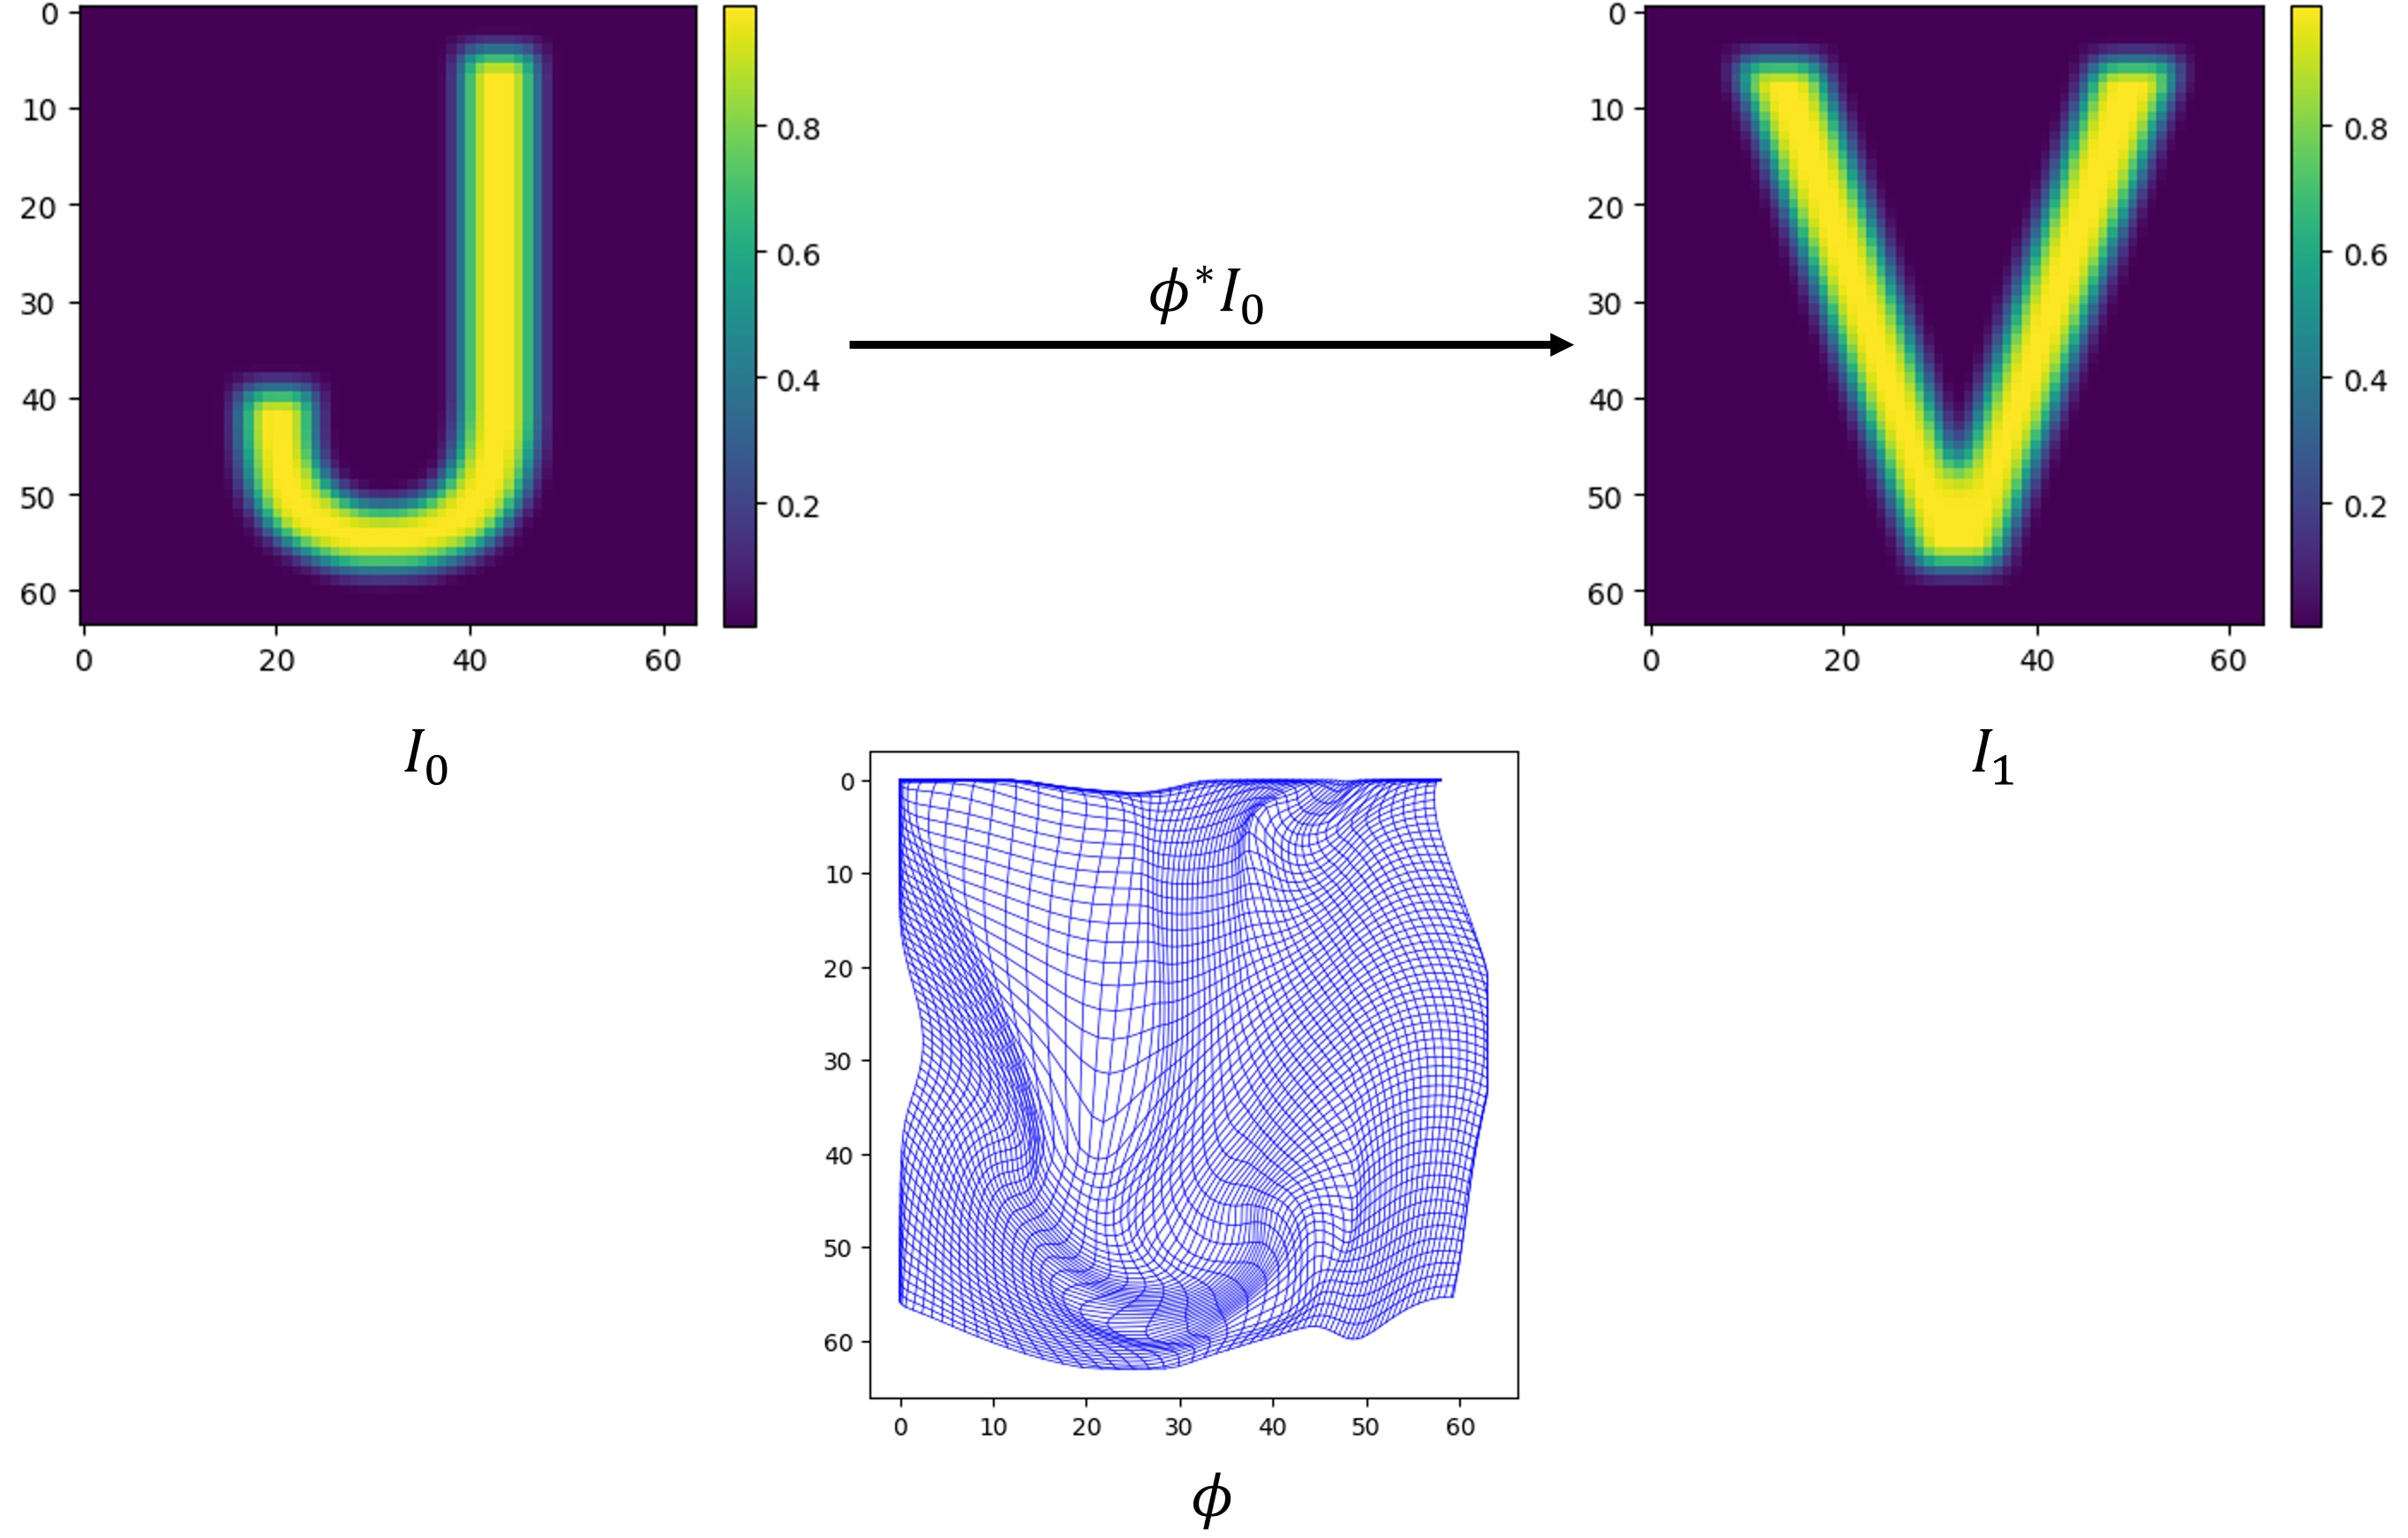
\includegraphics[scale=0.15]{figure/pullbackphi.png}
\caption{Pullback}
\end{figure}

\begin{figure}[H]
\centering
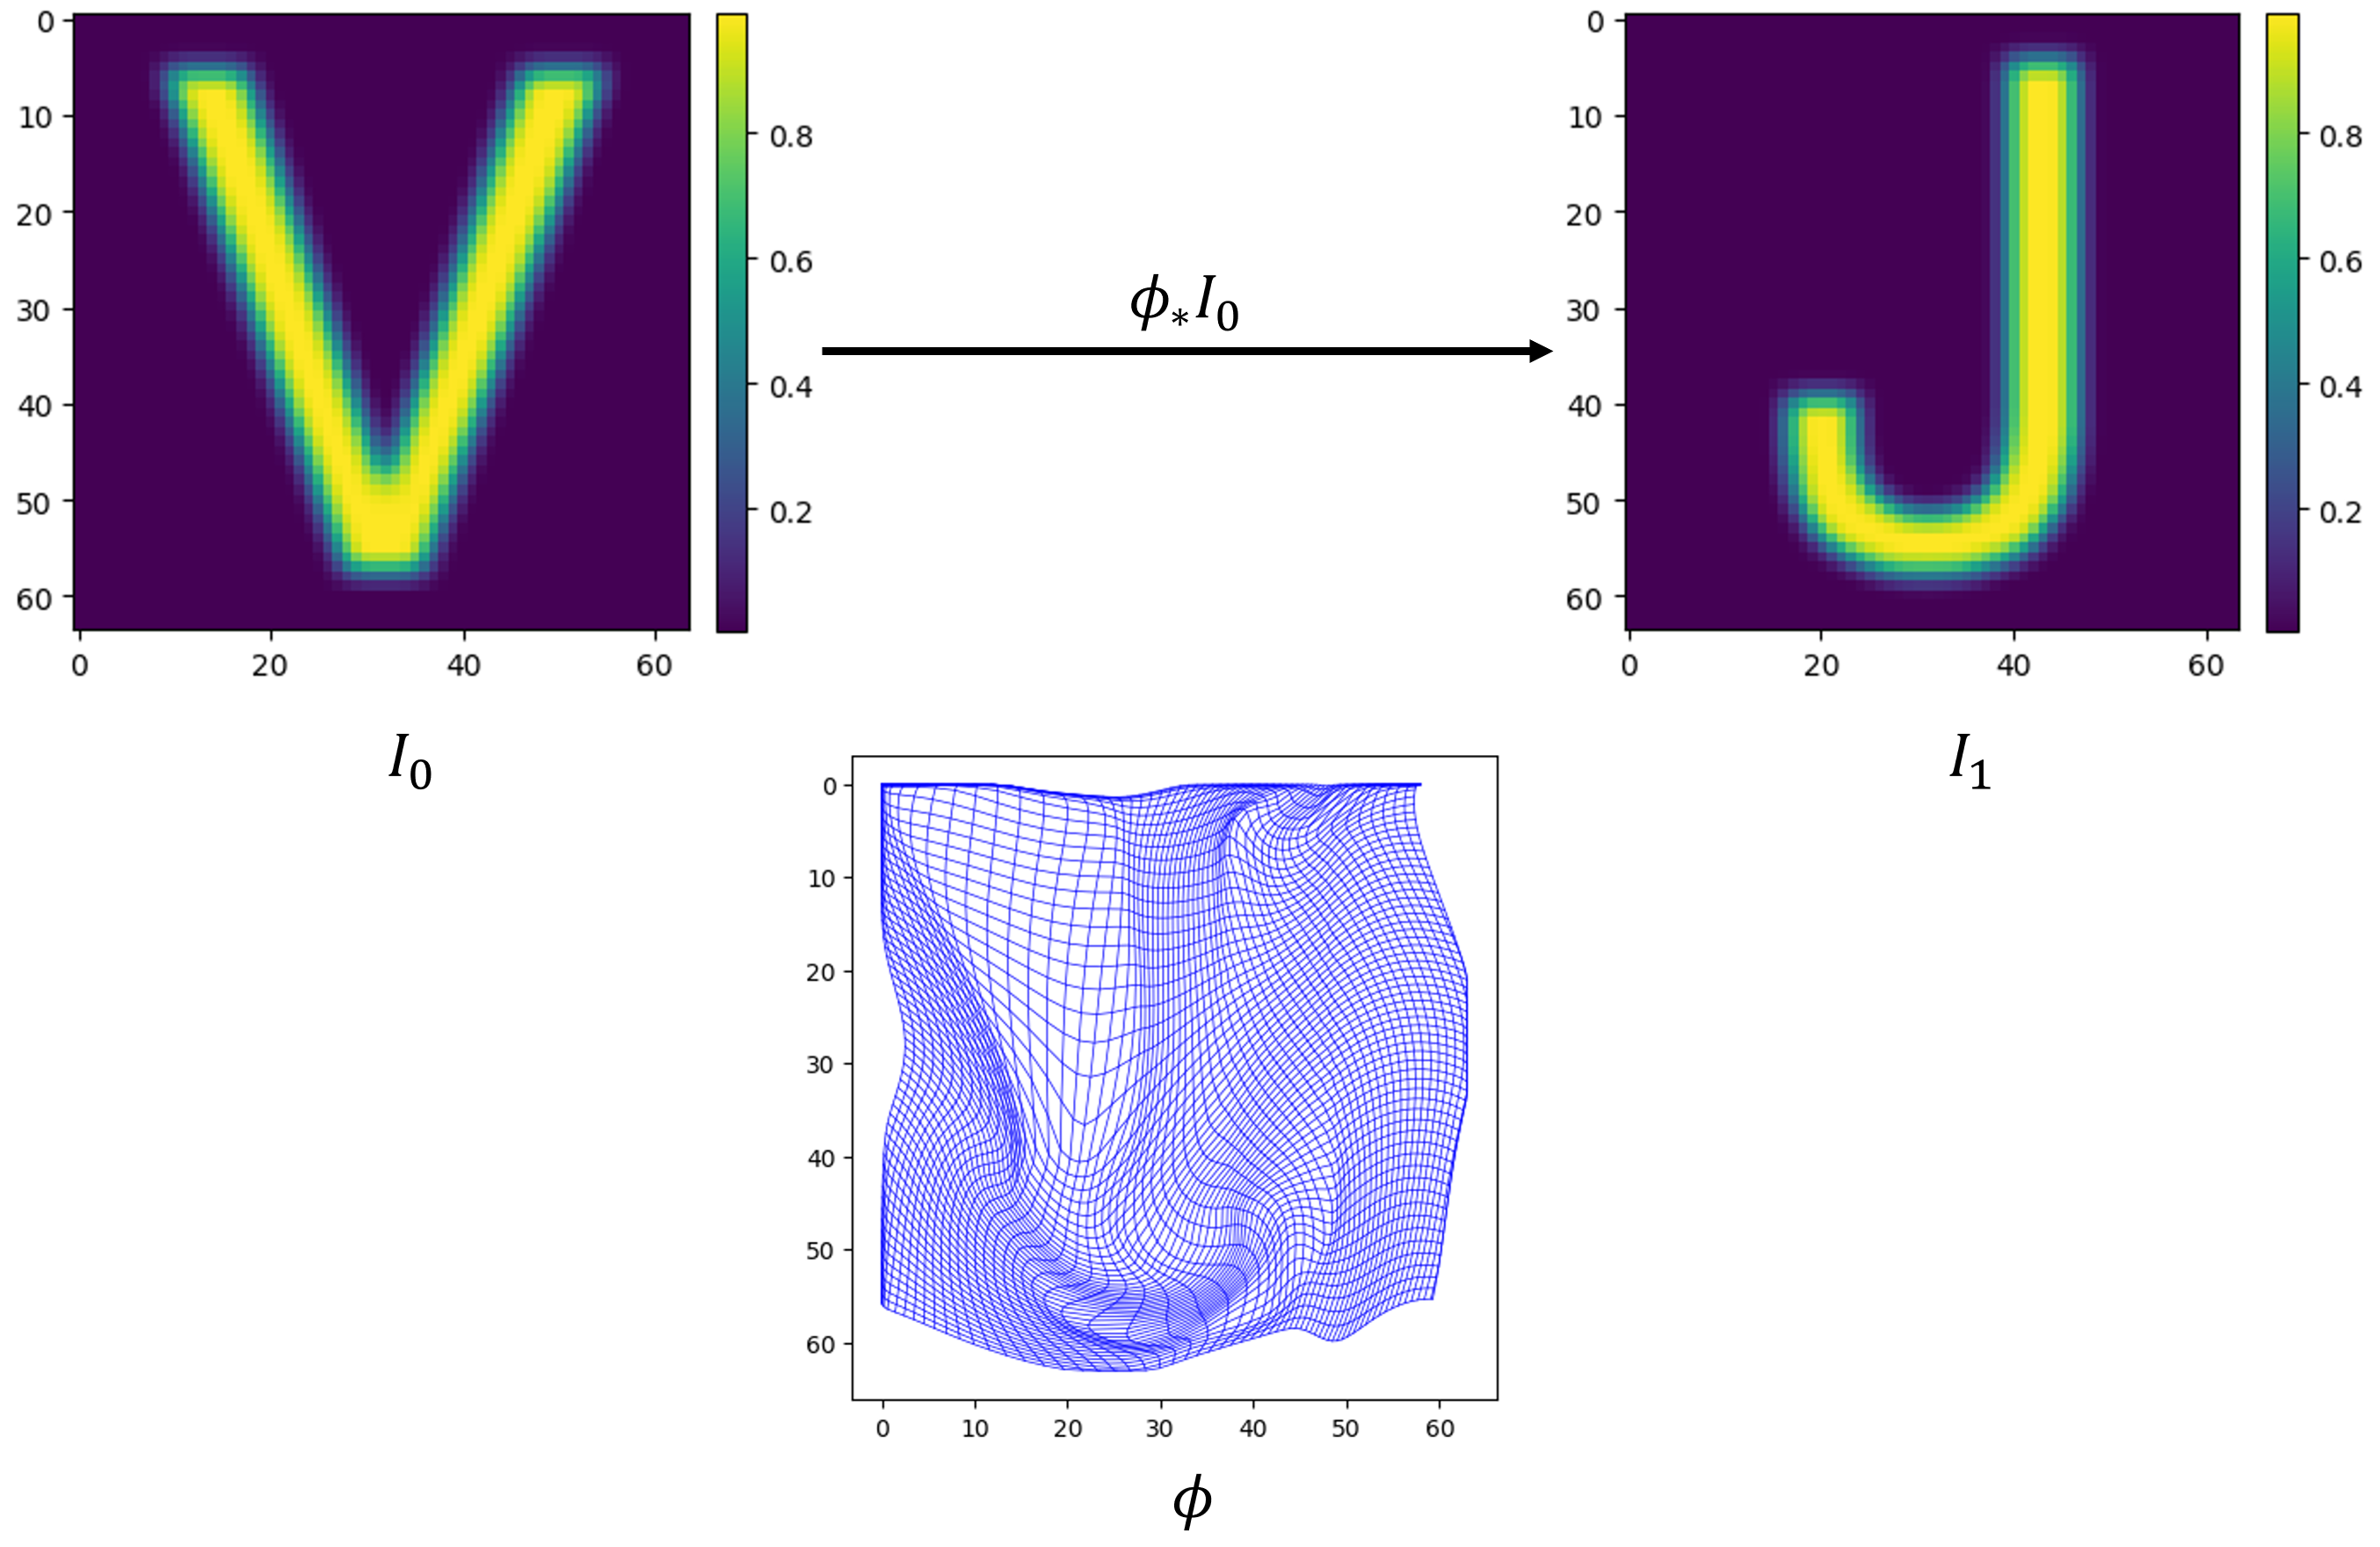
\includegraphics[scale=0.15]{figure/pushforwardphi.png}
\caption{Pushforward}
\end{figure}

\begin{remark}
\textbf{Relationship between $I_0, I_1, \phi, \phi^{-1}$:}
Intuitively, we may think that $\phi$ demonstrate the right way to distort $I_0:V$ to $I_1:J$, like distorting the ``painted flat tablecloth''. In a sense, that's right, if we write it as $I_1=\phi_*I_0$. However, we always use compose operation to distort the density map, which is $|D\phi^{-1}|I_0\circ\phi^{-1}$, so when we are using the composing, always remember that we are composing $\phi^{-1}$, instead of the more intuitively-correct $\phi$.
\end{remark}

\begin{figure}[H]
\centering
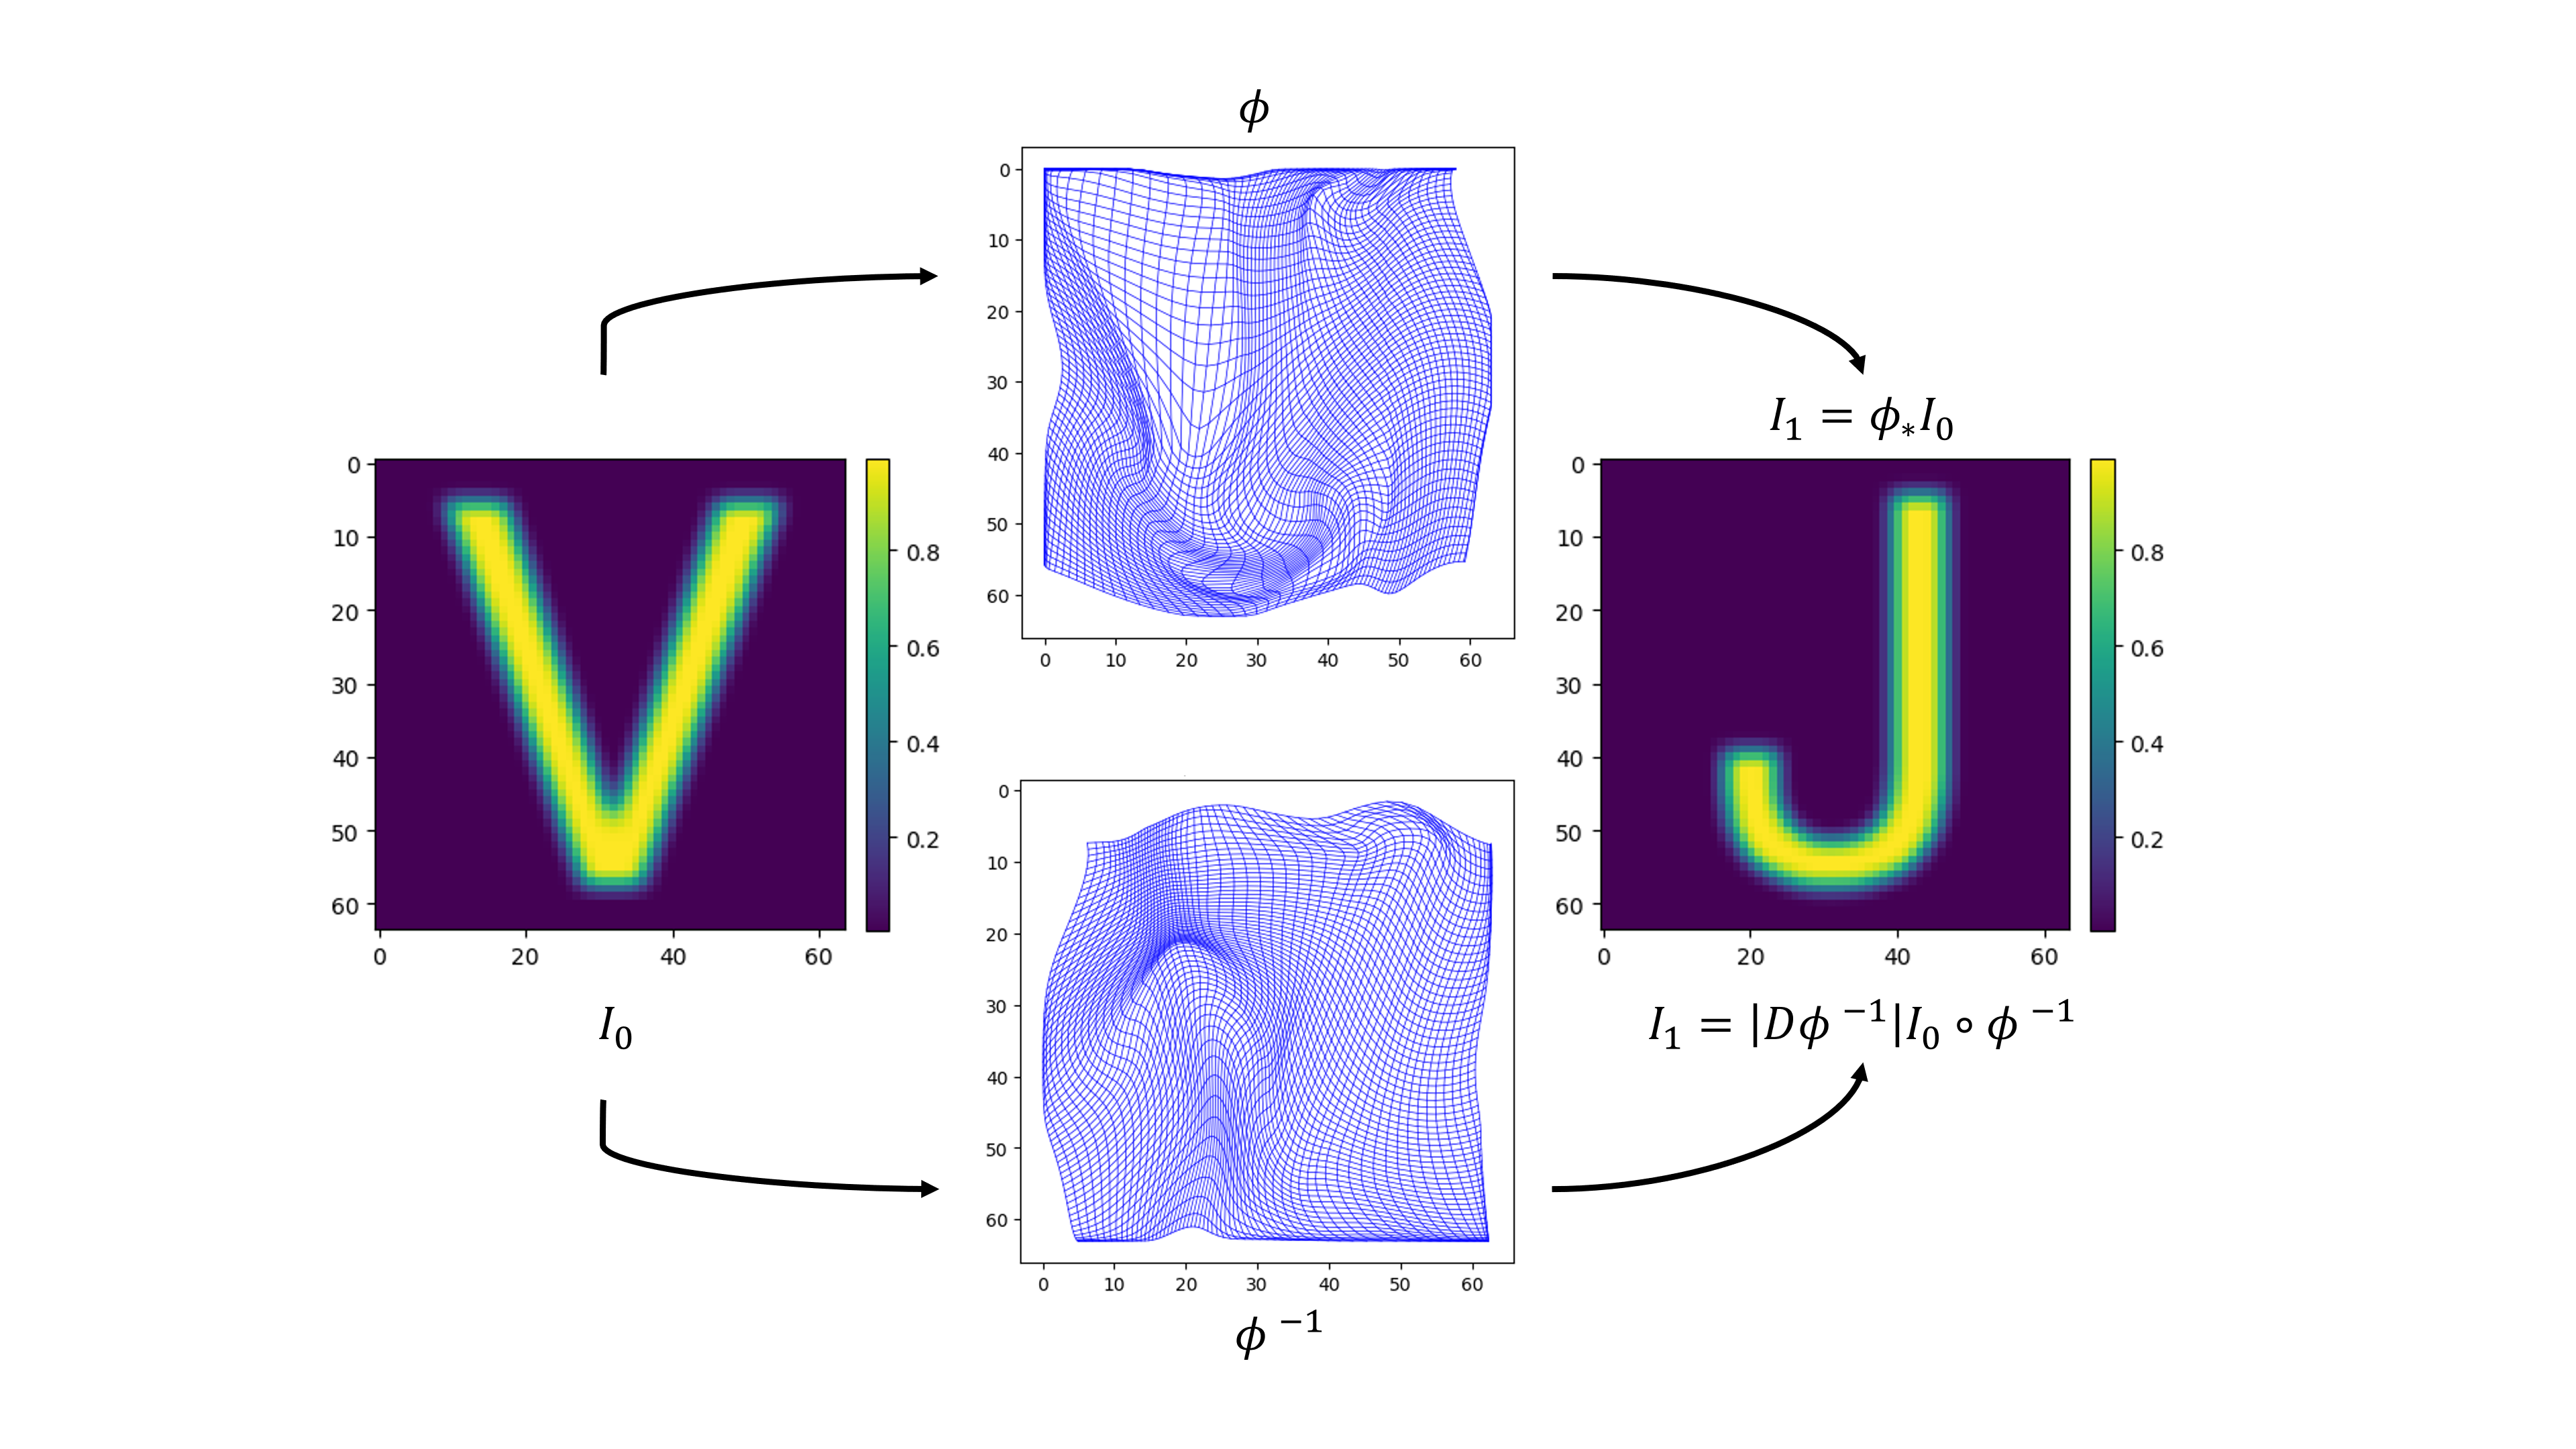
\includegraphics[scale=0.11]{figure/pushforward.png}
\caption{Pushforward}
\end{figure}

\begin{remark}
\textbf{``Blank Space''}
You may have the confusion that if we deform the image using the diffeomorphism $\varphi$ in Fig.(31), namely $\phi_*I$, what to fill in the blank triangle area at the bottom, since I analogize the diffeomorphism to distorting the ``painted flat tablecloth''.

How about we think this way, by implementing the algorithm through Python discretely, we can have $I\circ\varphi^{-1}:\mathbb{Z}^2\rightarrow\mathbb{R}^2\rightarrow\mathbb{R}$. The space of $\mathbb{Z}^2$ consists of all the integer tuple among $(0:M,0:N)$, where $M,N$ are the height and width of $I$. The space of $\mathbb{R}^2$ can be arbitrary real number tuple, but still in the range of $(0:M,0:N)$, as $I$ is not defined beyond this range. For simplicity, $I\circ\varphi^{-1}:\mathbb{Z}^2\rightarrow\mathbb{R}$ is still a function defined all over the $(0:M,0:N)$, which won't cause the blank space.

The essential cause of the above phenomena is that, due to the limitation in computer, we typically store the diffeomorphism in the data structure of array, which means $\phi:\mathbb{Z}^2\rightarrow\mathbb{R}^2$, where $\mathbb{Z}^2$ is consists of all the possible tuple among $(0:M,0:N)$, that's how we index the entries in the array. So we should never worry about the blank space, as how we plot the diffeomorphism is different from how to express it in algorithm.
\end{remark}

\begin{figure}[H]
\centering
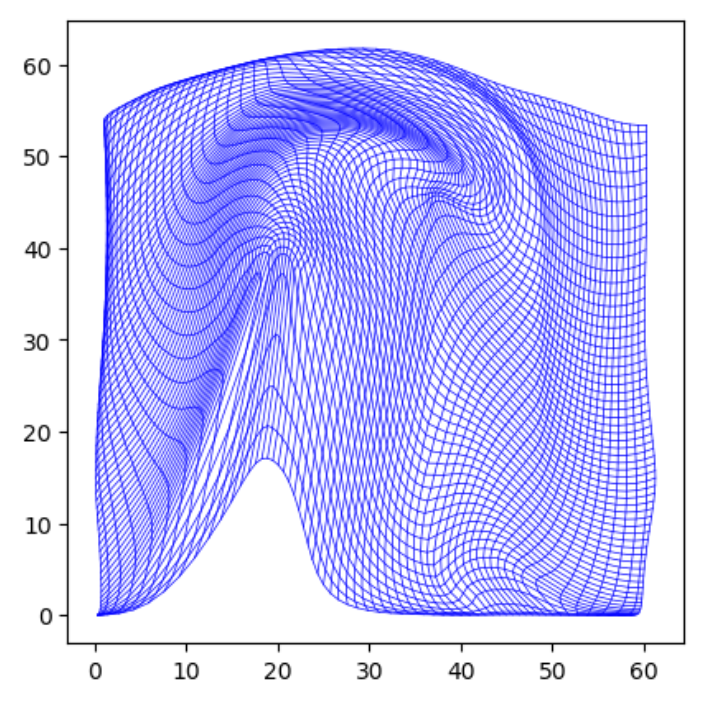
\includegraphics[scale=0.6]{figure/diffeo.png}
\caption{$\varphi$}
\end{figure}

\newpage
\section{Statistics}
\begin{definition}
\boxed{\textbf{Likelihood}} is the probability of certain observation given the reason, namely
\begin{equation*}
    p(\text{observation}|\text{reason}).
\end{equation*}
\end{definition}

\begin{definition}
\boxed{\textbf{Prior probability}} is the probability of the reason without any observation, namely
\begin{equation*}
    p(\text{reason}).
\end{equation*}
\end{definition}

\begin{definition}
\boxed{\textbf{Posterior probability}} is the probability of the reason with certain observation, namely
\begin{align*}
    p(\text{reason}|\text{observation})&=\frac{p(\text{observation}|\text{reason})}{p(\text{observation})}\times p(\text{reason})\\
    &\propto \text{Likelihood}\times\text{Prior Probability}
\end{align*}
\end{definition}

\begin{definition}
\boxed{\textbf{Probability mass function(PMF)}} is a function that gives the probability that a discrete random variable is exactly equal to some value.
\begin{equation*}
    P(X=a)=f(a).
\end{equation*}
\end{definition}

\begin{definition}
\boxed{\textbf{Probability density function(PDF)}} is a function the gives the probability of a continuous random variable is located among certain interval.
\begin{equation*}
    P(a\leq X\leq b)=\int _{a}^{b}f(x)\,dx.
\end{equation*}
\end{definition}

\begin{example}
Suppose bacteria of a certain species typically live 4 to 6 hours. The probability that a bacterium lives exactly 5 hours is equal to zero. A lot of bacteria live for approximately 5 hours, but there is no chance that any given bacterium dies at exactly 5.0000000000... hours. However, the probability that the bacterium dies between 5 hours and 5.01 hours is quantifiable. 
\end{example}

\begin{remark}
A PDF must be integrated over an interval to yield a probability.
\end{remark}

\begin{definition}
\boxed{\textbf{Maximum likelihood estimation (MLE)}} is a method of estimating the parameters of a probability distribution by maximizing a likelihood function, so that under the assumed statistical model the observed data is most probable.
\end{definition}

\begin{example}
Now suppose that there was only one coin but its $p$ could have been any value $0\le p\le 1$. The likelihood function to be maximized is
\begin{equation*}
    L(p)={\binom {80}{49}}p^{49}(1-p)^{31}
\end{equation*}
and the maximization is over all possible values $0\le p\le 1$.

By differentiating $L(p)$ with respect to $p$ and setting to zero, we yield that the maximum likelihood estimator for p is $\frac{49}{80}$.
\end{example}

\begin{definition}
\boxed{\textbf{Monte Carlo methods}} are a broad class of computational algorithms that rely on repeated random sampling to obtain numerical results. Monte Carlo methods vary, but tend to follow a particular pattern:
\begin{enumerate}
    \item Define a domain of possible inputs;
    \item Generate inputs randomly from a probability distribution over the domain;
    \item Perform a deterministic computation on the inputs;
    \item Aggregate the results.
\end{enumerate}
\end{definition}

\begin{example}
Consider a quadrant (circular sector) inscribed in a unit square. Given that the ratio of their areas is $\frac{\pi}{4}$, the value of $\pi$ can be approximated using a Monte Carlo method:
\begin{enumerate}
    \item Draw a square, then inscribe a quadrant within it;
    \item Uniformly scatter a given number of points over the square;
    \item Count the number of points inside the quadrant, i.e. having a distance from the origin of less than 1. The ratio of the inside-count and the total-sample-count is an estimate of the ratio of the two areas, namely the approximation of $\frac{\pi}{4}$;
    \item Multiply the result by 4 to estimate $\pi$.
\end{enumerate}
\begin{figure}[H]
    \centering
    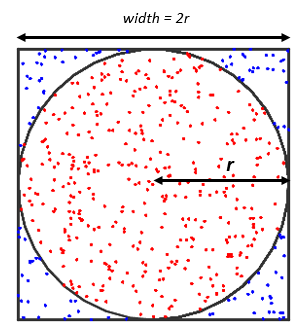
\includegraphics[scale=0.7]{figure/estimating-pi-monte-carlo-method.png}
    % \caption{Caption}
    % \label{fig:my_label}
\end{figure}
\end{example}

\begin{definition}
\boxed{\textbf{Normal distribution}} $X\sim N(\mu,\sigma^2)$ is defined as 
\begin{equation*}
     f(x)=\frac{1}{\sqrt{2\pi}}e^{-\frac{(x-\mu)^2}{2\sigma^2}}, F(x)=\int_0^\infty\frac{1}{\sqrt{2\pi}}e^{-\frac{(x-\mu)^2}{2\sigma^2}}dx,
 \end{equation*}
 where $\mu$ is the mean value and $\sigma$ is the standard deviation.
\end{definition}

\begin{remark}
Some properties of normal distribution:
\begin{itemize}
    \item If $X\sim N(\mu,\sigma^2), a, b$ are real, then $aX+b\sim N(a\mu+b,(a\sigma)^2)$.
    \item If $X\sim N(\mu_X,\sigma_X^2)$ and $Y\sim N(\mu_Y,\sigma_Y^2)$ are two independent random variables, then $ X+Y \sim N(\mu_X + \mu_Y, \sigma^2_X + \sigma^2_Y), {\displaystyle X-Y\sim N(\mu _{X}-\mu _{Y},\sigma _{X}^{2}+\sigma _{Y}^{2})}$.
\end{itemize}
\end{remark}

\begin{theorem}
\textbf{Law of large numbers (LLN).} When $\{X_1,\cdots,X_n\}$ is an infinite sequence of independent identical distributed random variables with expectation $E(X_1),\cdots,E(X_n)=\mu$, we can have
\begin{equation*}
    \Bar{X}_n\rightarrow\mu, \text{when }n\rightarrow\infty,
\end{equation*}
where $\Bar{X}_n=\frac{1}{n}\sum^n_{i=1} X_i$.
\end{theorem}

\begin{remark}
We can approximate the expectation of an unknown distribution by performing a sufficient number of the trials.
\end{remark}

\begin{figure}[H]
    \centering
    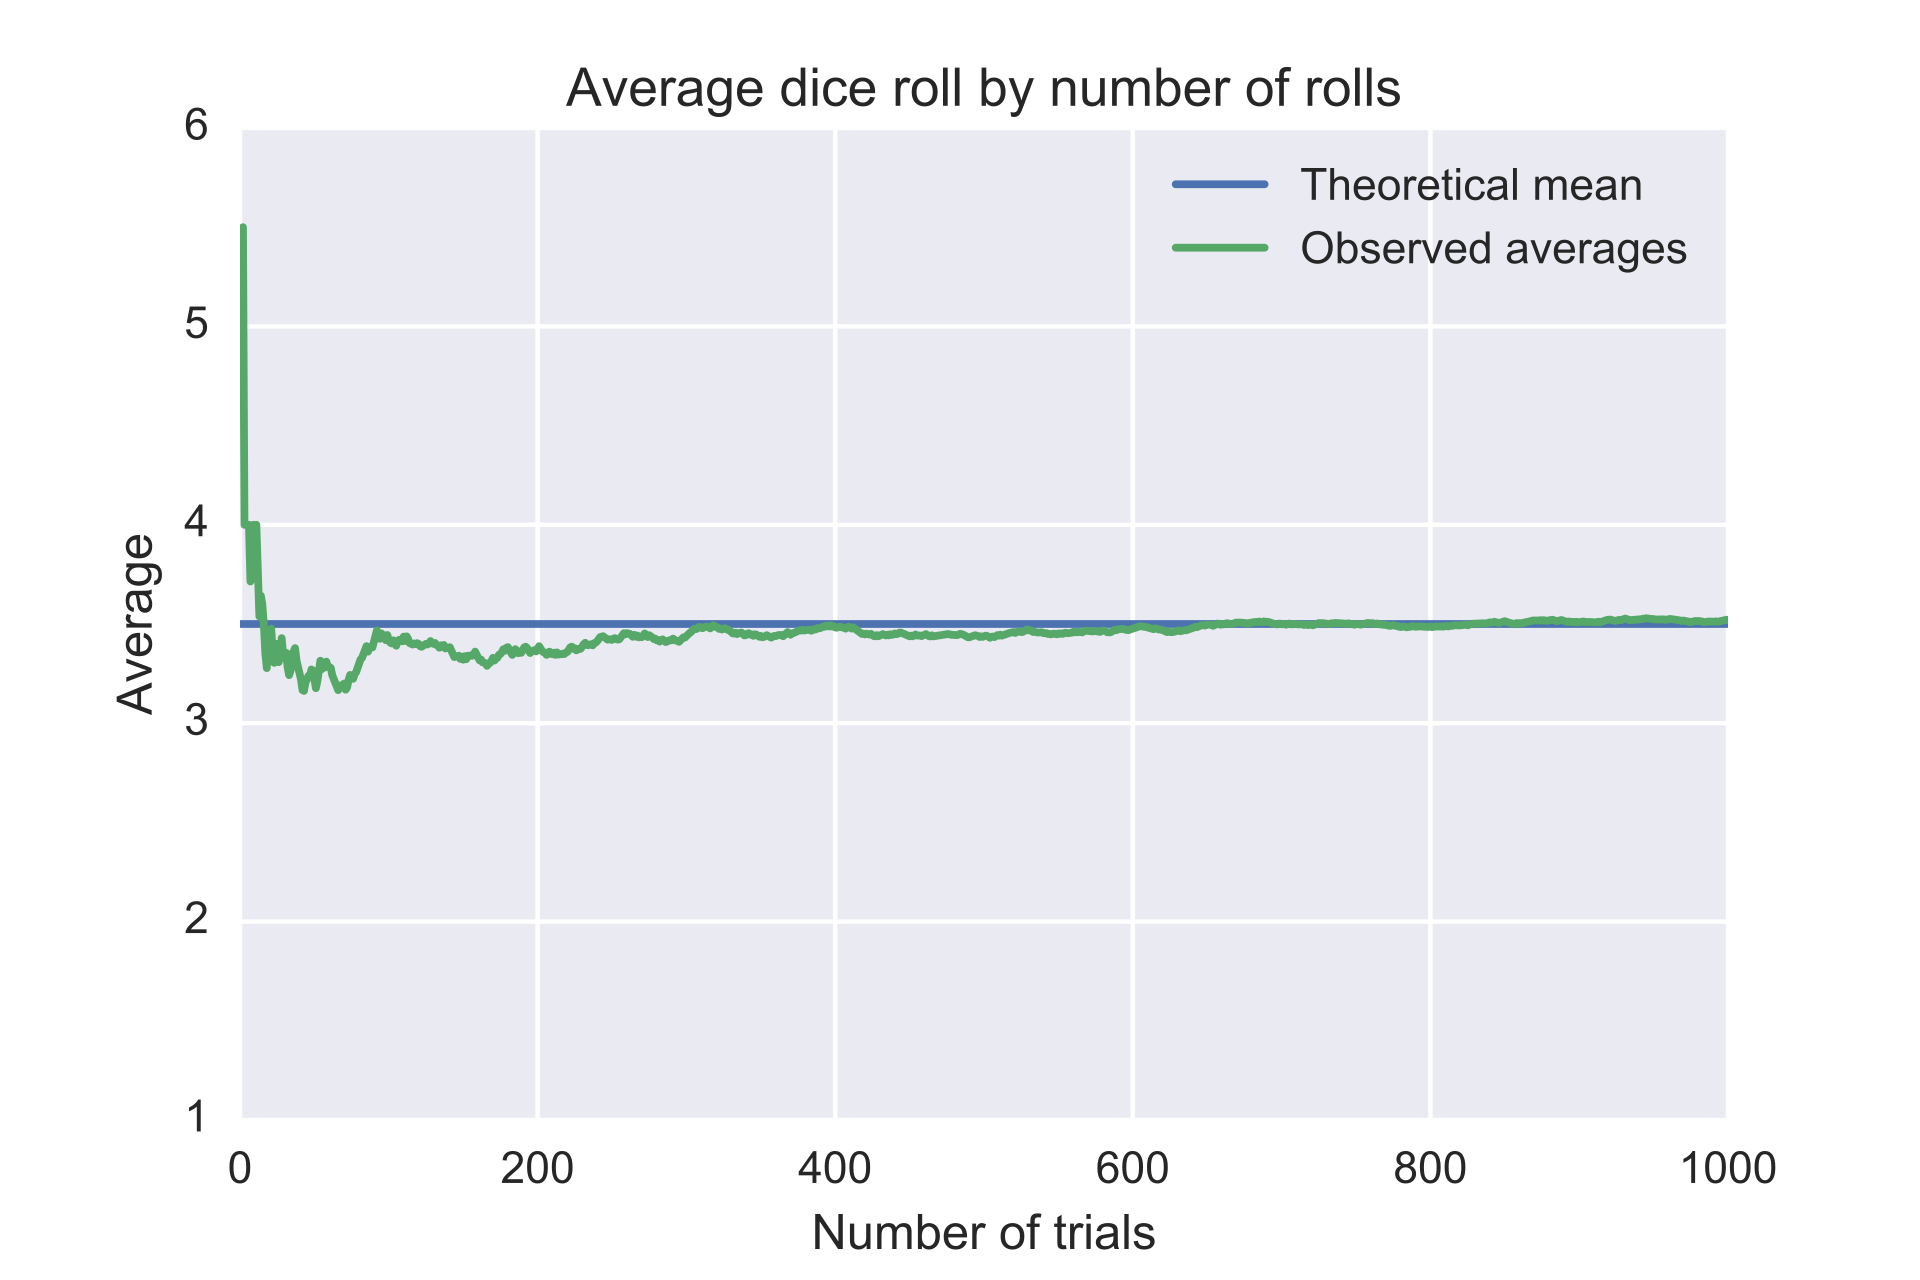
\includegraphics[scale=0.15]{figure/1920px-Lawoflargenumbers.svg.png}
    \caption{Law of large numbers}
    % \label{fig:my_label}
\end{figure}

\begin{theorem}
\textbf{Central limit theorem (CLT).} In many situation, when independent random variables are added, their properly normalized sum tends toward a normal distribution even if the original variables themselves are not normal distributed.
\end{theorem}

\begin{remark}
The theorem is a key concept in probability theory because this theorem allows us to leverage the normal distribution to solve other unknown distributions.
\end{remark}

\begin{example}
Given a sequence of i.i.d. random variables $\{X_1,\cdots,X_n\}$, we randomly pick $m$(relatively large) samples from the population to calculate the mean value and repeat it $k$ times. And the $k$ mean values would be normal distributed.
\end{example}

\begin{definition}
\boxed{\textbf{Confidence interval}} is defined as 

\end{definition}

\begin{definition}
\boxed{\textbf{Covariance}} for two random variables $X$ and $Y$, each with sample size $d$ is defined by
\begin{align*}
    \operatorname{cov}(X,Y)&=E[(X-E[X])(Y-E(Y])]\\
    &=\sum^d_{i=1}\frac{(x_i-\Bar{x})(y_i-\Bar{y})}{d}
\end{align*}
\end{definition}

\begin{definition}
\boxed{\textbf{Covariance matrix}} for $n$ sets of random variables $\{X^1\},\cdots,\{X^n\}$, each with sample size $d$ is defined by
\begin{align*}
    \Sigma=
    \begin{pmatrix}
        \operatorname{cov}(X^1,X^1) & \cdots & \operatorname{cov}(X^1,X^n)\\
        \vdots &  \ddots &  \vdots \\
        \operatorname{cov}(X^n,X^1) & \cdots & \operatorname{cov}(X^n,X^n)
    \end{pmatrix}
\end{align*}
\end{definition}

\begin{definition}
\boxed{\textbf{Principal components analysis(PCA)}} seeks a sequence of linear subspaces that maximize the variance of the data, the intent of which is to find an orthonormal basis $\{e_1,\cdots,e_k\}$ of a set of points $\{S^1,\cdots,S^n\}\in\mathbb{R}^d$, and the new basis is of the same dimension $d$ as the original space, which satisfies the recursive relationship
\begin{align*}
    e_1&=\argmax_{\|e\|=1}\sum^n_{i=1}\langle e,S^i\rangle^2\\
    e_2&=\argmax_{\|e\|=1}\sum^n_{i=1}[\langle e_1,S^i\rangle^2+\langle e,S^i\rangle^2]\\
    \vdots\\
    e_k&=\argmax_{\|e\|=1}\sum^n_{i=1}[\langle e_1,S^i\rangle^2+\cdots+\langle e_{k-1},S^i\rangle^2+\langle e,S^i\rangle^2]
\end{align*}
In other words, the subspace $V_k=\operatorname{span}(\{e_1,\cdots,e_k\})$ is the $k$-dimensional subspace that maximizes the variance of the data projected to the subspace. The basis $\{e_i\}$ is computed as the set of ordered eigenvectors of the sample covariance matrix of the data.
\end{definition}

\begin{remark}
Concatenating all the feature vector together as a matrix, using SVD to decompose the matrix is a common way of performing PCA.
\end{remark}

\begin{example}
Given a dataset $S=\{S^1,\cdots,S^n\}$ of $n$ samples, where $S^i\in\mathbb{R}^d$ and $\Bar{S}$ is the mean of the dataset $S$
\begin{equation*}
    S^i=
    \begin{pmatrix}
        s^i_1\\
        \vdots\\
        s^i_d
    \end{pmatrix},
    \Bar{S}=
    \begin{pmatrix}
        \Bar{s}_1\\
        \vdots\\
        \Bar{s}_d
    \end{pmatrix}.
\end{equation*}
Then we can have a $d\times d$ covariance matrix $\Sigma$
\begin{equation*}
    \Sigma=
    \begin{pmatrix}
        \operatorname{cov}(s_1,s_1) & \cdots & \operatorname{cov}(s_1,s_d)\\
        \vdots &  \ddots &  \vdots \\
        \operatorname{cov}(s_d,s_1) & \cdots & \operatorname{cov}(s_d,s_d)
    \end{pmatrix}=
    \begin{pmatrix}
        \text{cov of $1^{st}$ and $1^{st}$ dim} & \cdots & \text{cov of $1^{st}$ and $d^{th}$ dim}\\
        \vdots &  \ddots &  \vdots \\
        \text{cov of $d^{th}$ and $1^{st}$ dim} & \cdots & \text{cov of $d^{th}$ and $d^{th}$ dim}
    \end{pmatrix},
\end{equation*}
where
\begin{equation*}
    \operatorname{cov}(s_j,s_k)=\frac{\sum^n_{i=1}(s^i_j-\Bar{s}_j)(s^i_k-\Bar{s}_k)}{n}.
\end{equation*}
To form a reduced dimension space $S'$, simply pick the largest $k$ eigenvalues of the covariance matrix above and the corresponding eigenvectors and the new dataset $S'$ is formed as below
\begin{equation*}
    \underbrace{
    \begin{pmatrix}
        S'^1 & \cdots & S'^n
    \end{pmatrix}}_{k\times n}=
    \underbrace{
    \begin{pmatrix}
        e^T_1\\
        \vdots\\
        e^T_p
    \end{pmatrix}}_{k\times d}\cdot
    \underbrace{
    \begin{pmatrix}
        S^1 & \cdots & S^n
    \end{pmatrix}}_{d\times n}
\end{equation*}
\end{example}

\begin{definition}
\boxed{\textbf{Principal geodesic analysis(PGA)}} seeks a sequence of geodesic submanifolds that maximize the variance of the data. These submanifolds are called the principal geodesic submanifolds.
\begin{itemize}
    \item \textbf{Definition 1.} The principal geodesic submanifolds are defined by first constructing an orthonormal basis $e_1,\cdots,e_d$ of $T_\mu M$. Then, these vectors are used to form a sequence of nested subspaces $V_k=\operatorname{span}(\{e_1,\cdots,e_k\})\cap U$, where $U\subset T_\mu M$ is a neighbourhood of 0, such that projection is well-defined for all geodesic submanifolds of $\operatorname{Exp}_\mu(U)$. 
    
    The principal geodesic submanifolds are given by 
    \begin{equation*}
        H_k=\operatorname{Exp}_\mu(V_k)
    \end{equation*}
    The first principal direction is now chosen to maximize the projected variance along the corresponding geodesic:
    \begin{align*}
        e_1&=\argmax_{\|e\|=1}\sum^n_{i=1}\|\operatorname{Log}_\mu(\pi_H(x_i))\|^2, &&\text{where } H=\operatorname{Exp}_\mu(\operatorname{span}(\{e\})\cap U)\\
        e_k&=\argmax_{\|e\|=1}\sum^n_{i=1}\|\operatorname{Log}_\mu(\pi_H(x_i))\|^2, &&\text{where } H=\operatorname{Exp}_\mu(\operatorname{span}(\{e_1,\cdots,e_{k-1},e\})\cap U)\\
    \end{align*}
    where we define the \textbf{projection operator} $\pi_H:M\rightarrow H$ as
    \begin{align*}
        \pi_H(x)&=\argmin_{y\in H}d(x,y)^2\\ 
        &=\argmin_{y\in H}\|\operatorname{Log}_x(y)\|^2\\
        &\approx\argmin_{y\in H}\|\operatorname{Log}_p(x)-\operatorname{Log}_p(y)\|^2
    \end{align*}
    
    \item \textbf{Definition 2.} The intent of principal geodesic analysis is to find an orthonormal basis $\{e_1,\cdots,e_k\}$ of a set of points $\{x_1,\cdots,x_n\}\in\mathbb{R}^d$, which satisfies the recursive relationship
    \begin{align*}
        e_1&=\argmin_{\|e\|=1}\sum^n_{i=1}\|x_i-\langle e,x_i\rangle e\|^2\\
        e_2&=\argmin_{\|e\|=1}\sum^n_{i=1}\|x_i-\langle e_1,x_i\rangle e_1-\langle e,x_i\rangle e\|^2\\
        \vdots\\
        e_k&=\argmin_{\|e\|=1}\sum^n_{i=1}\|x_i-\langle e_1,x_i\rangle e_1-\cdots-\langle e_{k-1},x_i\rangle e_{k-1}-\langle e,x_i\rangle e\|^2
    \end{align*}
    In other words, the subspace $V_k=\operatorname{span}(\{e_1,\cdots,e_k\})$ is the $k$-dimensional subspace that minimizes the sum-of-squared distances to the data.
    The principal geodesic submanifolds are given by 
    \begin{equation*}
        H_k=\operatorname{Exp}_\mu(V_k)
    \end{equation*}
    The first principal direction is now chosen to minimize the sum-of-squared distance of the data to the corresponding geodesic:
    \begin{align*}
        e_1&=\argmax_{\|e\|=1}\sum^n_{i=1}\|\operatorname{Log}_{x_i}(\pi_H(x_i))\|^2, &&\text{where } H=\operatorname{Exp}_\mu(\operatorname{span}(\{e\})\cap U)\\
        e_k&=\argmax_{\|e\|=1}\sum^n_{i=1}\|\operatorname{Log}_{x_i}(\pi_H(x_i))\|^2, &&\text{where } H=\operatorname{Exp}_\mu(\operatorname{span}(\{e_1,\cdots,e_{k-1},e\})\cap U)\\
    \end{align*}
\end{itemize}
\end{definition}

\begin{example}
\begin{algorithm}[H]
\caption{Principal Geodesic Analysis}\label{algoKM}
    \begin{algorithmic}
    \Inputs{$x_1,\cdots,x_n\in M$}
        \State $\mu\leftarrow\text{intrinsic mean of }\{x_i\}$\Comment{Remark \ref{intrinsicmean}}
        \State $u_i\leftarrow\operatorname{Log}_\mu(x_i)$\Comment{Map $x_i\in M$ to $T_\mu M$ as $u_i$}
        \State $\Sigma\leftarrow \frac{1}{n}\sum^n_{i=1}u_iu_i^T$
        \State $\{e_k,\lambda_k\}\leftarrow \text{eigenvectors and eigenvalues of }\Sigma$
        \State \Return{$\{e_k,\lambda_k\}$}
    \end{algorithmic}
\end{algorithm} 
\end{example}

\begin{remark}
\begin{itemize}
    \item The sample variance of the data is the expected value of the squared Riemannian distance from the mean.
    \item For data in $\mathbb{R}^n$ the two definitions are equivalent since PGA reduces to PCA in the linear case.
\end{itemize}
\end{remark}

\begin{definition}
\boxed{\textbf{Fréchet mean and variance}} are defined as
\begin{align*}
    p_*&=\argmin_p\phi(p), && \triangleright\text{Fréchet mean}\\
    \phi(p)&=\sum^N_{i=1}d^2(p,x_i)w_i, && \triangleright\text{Fréchet variance}
\end{align*}
where $(M,d)$ is a complete metric space, $x_1,x_2,\cdots,x_n$ are the random points in $M$ and $p\in M$.
\end{definition}

\begin{remark}
The \textbf{Karcher} means are then those points, $p$ of $M$, which locally minimize $\phi$, while the \textbf{Fréchet} means are then those points, which globally minimize $\phi$.
\end{remark}

\begin{remark}
Actually, the Fréchet mean is the generalization of the arithmetic mean, median, geometric mean, and harmonic mean, by using different distance functions.
\begin{itemize}
    \item For real numbers, the \textbf{arithmetic} mean is a Fréchet mean, by using the usual Euclidean distance as the distance function.
    \item For positive real numbers, the \textbf{geometric} mean is a Fréchet mean, by using the (hyperbolic) distance function $d(x,y)=|\log(x)-\log(y)|$
    \item For positive real numbers, the \textbf{harmonic} mean is a Fréchet mean, by using the distance function $d(x,y)=|\frac{1}{x}-\frac{1}{y}|$
\end{itemize}
\end{remark}

\begin{remark}\label{intrinsicmean}
\textbf{How to compute the intrinsic mean of manifold data:} According to 4.1.2 in \cite{tomthesis}, Karcher\cite{karcher} shows that the gradient of $\phi$ above is
\begin{equation*}
    \nabla\phi(p)=-2\sum^N_{i=1}\operatorname{Log}_p(x_i)w_i.
\end{equation*}
If $w_i=\frac{1}{2N}$, then we have
\begin{align*}
    \phi(p)&=\frac{1}{2N}\sum^N_{i=1}d^2(p,x_i),\\
    \nabla\phi(p)&=-\frac{1}{N}\sum^N_{i=1}\operatorname{Log}_p(x_i).
\end{align*}
The gradient descent algorithm takes successive steps in the negative gradient direction. Given a current estimate $\mu_j$, say $\mu_1=x_1$, as the intrinsic mean, the equation for updating the mean by taking a step in the negative gradient direction is
\begin{equation*}
    \mu_{j+1}=\operatorname{Exp}_{\mu_j}\left(\frac{\tau}{N}\sum^N_{i=1}\operatorname{Log}_{\mu_j}(x_i)\right),
\end{equation*}
where $\tau$ is the step size.
And this updating equation is easy to understand: Log map all the $x_i\in M$ to the tangent space of $\mu_j$, after derived the mean in the tangent space, exp map this mean back to the $M$, namely the final intrinsic mean we want.
\end{remark}

\begin{definition}
\boxed{\textbf{Fréchet median}} is defined as
\begin{align*}
    p_*&=\argmin_p\psi(p), && \triangleright\text{Fréchet median}\\
    \psi(p)&=\sum^N_{i=1}|d^2(p,x_i)|,
\end{align*}
where $x_1,x_2,\cdots,x_n$ are the random points in $M$ and $p\in M$.
\end{definition}

\begin{definition}
\boxed{\textbf{Weighted geometric median}} is defined as
\begin{align*}
    p_*&=\argmin_p\psi(p),\\
    \psi(p)&=\sum^N_{i=1}d^2(p,x_i)w_i,
\end{align*}
where $x_1,x_2,\cdots,x_n$ are the random points in $M$ and $p\in M$.
\end{definition}

\begin{corollary}
Given $\Delta f=g$, $f(x,y)=\mathcal{F}^{-1}\left[\frac{1}{2\cos(2\pi u/M)+2\cos(2\pi v/N)-4}G(u,v)\right]$.
\begin{proof}
\begin{align*}
    f(x+1,y)+f(x-1,y)+f(x,y+1)+f(x,y-1)-4f(x,y)&=g(x,y)\\
    \mathcal{F}[f(x+1,y)+f(x-1,y)+f(x,y+1)+f(x,y-1)-4f(x,y)]&=\mathcal{F}[g(x,y)]\\
    e^{-2\pi ju/M}F(u,v)+e^{2\pi ju/M}F(u,v)+e^{-2\pi jv/N}F(u,v)+e^{2\pi jv/N}F(u,v)-4F(u,v)&=G(u,v)\\
    \triangleright\text{time shifting\cite{shift}: }\mathcal{F}(f(x+a,y+b))=e^{-2\pi jau/M-2\pi jbv/N}F(u,v)
\end{align*}

After withdrawing the common factor, we have
\begin{align*}
    F(u,v)&=\frac{1}{e^{-2\pi ju/M}+e^{2\pi ju/M}+e^{-2\pi jv/N}+e^{2\pi jv/N}-4}G(u,v)\\
    f(x,y)&=\mathcal{F}^{-1}\left[\frac{1}{e^{-2\pi ju/M}+e^{2\pi ju/M}+e^{-2\pi jv/N}+e^{2\pi jv/N}-4}G(u,v)\right]
\end{align*}

As $e^{ju}=\cos(u)+j\sin(u)$, we can write $f(x,y)$ in this way:
\begin{equation*}
    f(x,y)=\mathcal{F}^{-1}\left[\frac{1}{2\cos(2\pi u/M)+2\cos(2\pi v/N)-4}G(u,v)\right]
\end{equation*}

Likewise, you can find the 3D one like below:
\begin{equation*}
    f(x,y,z)=\mathcal{F}^{-1}\left[\frac{1}{2\cos(2\pi u/M)+2\cos(2\pi v/N)+2\cos(2\pi w/O)-6}G(u,v,w)\right]
\end{equation*}
\end{proof}
\end{corollary}

\begin{remark}
The formula below defines MATLAB's discrete Fourier transform $G$ of an $m\times n$ matrix $g$:
\begin{equation*}
    G(u,v)=\sum^{m}_{x=1}\sum^{n}_{y=1}w^{(x-1)(u-1)}_mw^{(y-1)(v-1)}_ng(x,y),
\end{equation*}
where $w_m=e^{-2\pi i/m},w_n=e^{-2\pi i/n}$ and $x,u\in[1,m], y,v\in[1,n]$.

In a more specific way, we have
\begin{equation*}
    G(u,v)=\sum^{m}_{x=1}\sum^{n}_{y=1}e^{-2\pi i\left(\frac{(x-1)(u-1)}{m}+\frac{(y-1)(v-1)}{n}\right)}g(x,y)
\end{equation*}
\end{remark}

\newpage
\section{Linear Algebra}
\subsection{Multiplication}
\begin{definition}
Matrix multiplication of $U,V$ can be presented by two ways
\begin{align*}UV&=
    \begin{pmatrix}
        \langle u_1,v^1\rangle & \langle u_1,v^2\rangle & \cdots &\langle u_1,v^n\rangle \\
        \langle u_2,v^1\rangle & \langle u_2,v^2\rangle & \cdots &\langle u_2,v^n\rangle \\
        \vdots & \vdots & \ddots &\vdots \\
        \langle u_n,v^1\rangle & \langle u_n,v^2\rangle & \cdots &\langle u_n,v^n\rangle \\
    \end{pmatrix}&&\triangleright\text{inner product}\\
    &=\sum^n_{i=1}\sum^n_{i=1}u^i\otimes v^i&&\triangleright\text{outer product}
\end{align*}
where the superscript indexes the columns and the subscript indexes rows.
\end{definition}
\subsection{Eigen}
\begin{definition}
If $v,\lambda$ satisfy $Av=\lambda v$, then $v,\lambda$ are \boxed{\textbf{eigenvalue and eigenvector}} of $A$.
\begin{align*}
    Av&=\lambda v\\
    Av-\lambda v&=0\\
    (A-\lambda I)v&=0\\
    |A-\lambda I|&=0
\end{align*}
\end{definition}

\begin{figure}[H]
    \centering
    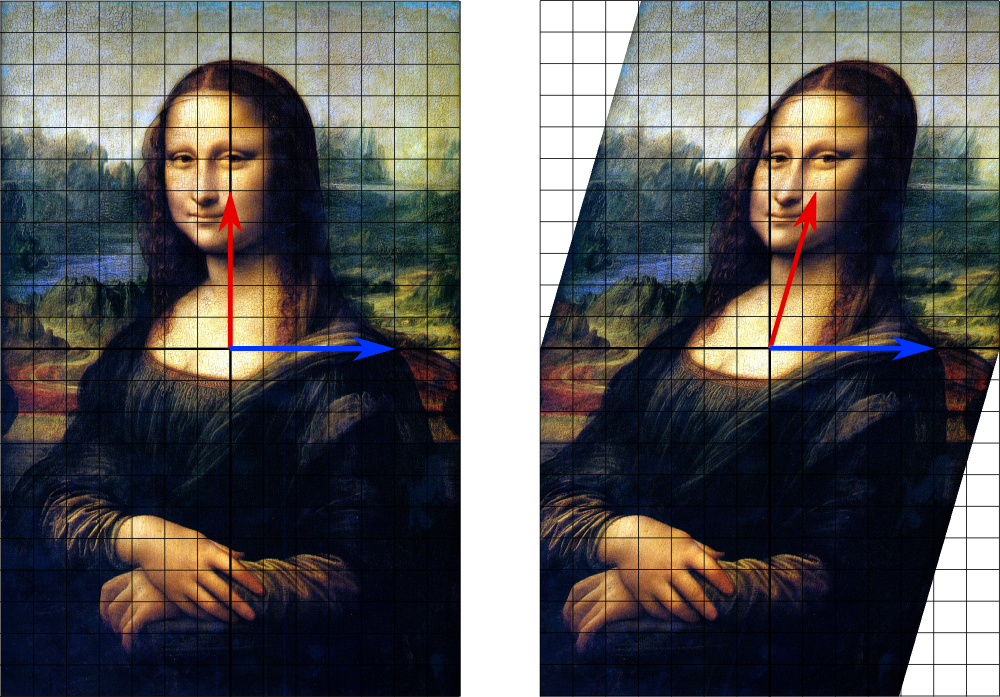
\includegraphics[scale=0.05]{figure/monalisa.png}
    \caption{In this shear mapping the red arrow changes direction, but the blue arrow does not. The blue arrow is an eigenvector of this shear mapping because it does not change direction, and since its length is unchanged, its eigenvalue is 1.}
    \label{fig:my_label}
\end{figure}

\begin{remark}
\begin{align*}
    \prod_i\lambda_i&=\operatorname{det}(A)\\
    \sum_i \lambda_i&=\operatorname{tr}(A)
\end{align*}

\begin{remark}
Let $A$ be a square $n\times n$ matrix with $n$ linearly independent eigenvectors $v_i$. Then $A$ can be factorized as
\begin{equation*}
    A=Q\Lambda Q^{-1},
\end{equation*}
where $Q$ is the square $n\times n$ matrix whose $i$-th column is the eigenvector $v_i$ of $A$, and $\Lambda$ is the diagonal matrix whose diagonal elements are the corresponding eigenvalues, $\Lambda_{ii}= \lambda_i$. Note that only diagonalizable matrices can be factorized in this way. For example, the defective matrix cannot be diagonalized.
\end{remark}

\end{remark}

\subsection{Inverse}
\begin{itemize}
    \item $(AB)^{-1}=B^{-1}A^{-1}$
    \item $(ABC...)^{-1}=...C^{-1}B^{-1}A^{-1}$
    \item $(A^{-1})^T=(A^T)^{-1}$
    \item $(rA)^{-1}=r^{-1}A^{-1}$
\end{itemize}

\subsection{Transpose}
\begin{itemize}
    \item $(AB)^T=B^TA^T$
    \item $(ABC...)^T=...C^TB^TA^T$
    \item $(A+B)^T=A^T+B^T$
    \item $(A^{-1})^T=(A^T)^{-1}$
    \item $(rA)^T=rA^{-1}$
\end{itemize}

\subsection{Trace}
\begin{itemize}
    \item $\operatorname{tr}(AB)=\operatorname{tr}(BA)$
    \item $\operatorname{tr}(ABC)=\operatorname{tr}(BCA)=\operatorname{tr}(CAB)$
    \item $\operatorname{tr}(A+B)=\operatorname{tr}(A)+\operatorname{tr}(B)$
    \item $\operatorname{tr}(A^T)=\operatorname{tr}(A)$
    \item $\operatorname{tr}(rA)=r\operatorname{tr}(A)$
    \item $\operatorname{tr}(P^{-1}AP)=\operatorname{tr}(A)$
\end{itemize}

\subsection{Determinant}
\begin{itemize}
    \item $\operatorname{det}(AB)=\operatorname{det}(A)\operatorname{det}(B)$
    \item $\operatorname{det}(A^{-1})=\operatorname{det}(A)^{-1}$, if $A$ is invertable
    \item $\operatorname{det}(A^T)=\operatorname{det}(A)$
    \item $\operatorname{det}(rA)=r^n\operatorname{det}(A)$
    \item $\operatorname{det}(A)=\prod\lambda_i$
    \item $\operatorname{det}(A)=\prod a_{ii}$, and $a_{ii}$ are the eigenvalues of $A$, if $A$ is triangular or diagonal
    \item $\operatorname{det}(A)A^{-1}=\operatorname{adj}(A)$
\end{itemize}

\begin{align*}
    &A\text{ is invertible}\Leftrightarrow\operatorname{det}(A)\not=0\Leftrightarrow\text{full rank}\Leftrightarrow\text{nonsingular}\Leftrightarrow\text{each column linearly independent}\\
    &A\text{ is non-invertible}\Leftrightarrow\operatorname{det}(A)=0\Leftrightarrow\text{rank deficient}\Leftrightarrow\text{singular}\Leftrightarrow\text{each column not linearly independent}
\end{align*}

\subsection{Logarithm}
\begin{itemize}
    \item $\log(AB)=\log A+\log B$
\end{itemize}

\subsection{Decomposition}
\begin{definition}
\boxed{\textbf{Orthogonal matrix.}} A square matrix $A\in\mathbb{R}^{n\times n}$ is called orthogonal if 
\begin{equation*}
    A^{-1}=A^T
\end{equation*}
\end{definition}

\begin{remark}
$A$ is orthogonal means rows or columns of $A$ are orthonormal(orthogonal and maganitude is 1) in $\mathbb{R}^{n\times n}$, $|\operatorname{det}(A)|=1, \|Ax\| = \|x\|.$ When $A$ is orthogonal and $\operatorname{det}(A)=1$, it's called rotation matrix.
\end{remark}

\begin{definition}
\boxed{\textbf{Cholesky decomposition.}} Let $A\in\mathbb{R}^{n\times n}$ be symmetric and positive definite. Then there exist a unique lower triangular matrix $L\in\mathbb{R}^{n\times n}$ with strictly positive diagonal entries such that
\begin{equation*}
    A=LL^T
\end{equation*}
\end{definition}

\begin{remark}
Using the Cholesky decomposition, we solve $LL^Tx=b$ instead of $Ax=b$ by
\begin{enumerate}
    \item Solving $Lz=b$ for $z$ using forward substitution
    \item Solving $L^Tx=z$ for $x$ using backward substitution
\end{enumerate}
\end{remark}

\begin{definition}
\boxed{\textbf{LU decomposition.}} Let $A\in\mathbb{R}^{n\times n}$ be invertable and let $A$ be diagonally dominant, namely $\forall i, |a_{ii}|\ge\sum_{i\not=j}|a_{ij}|$. Then there exist a lower triangular matrix $L\in\mathbb{R}^{n\times n}$ and a upper triangular matrix $U\in\mathbb{R}^{n\times n}$ such that
\begin{equation*}
    A=LU
\end{equation*}
\end{definition}

\begin{remark}
Using the LU decomposition, we solve $LUx=b$ instead of $Ax=b$ by
\begin{enumerate}
    \item Solving $Lz=b$ for $z$ using forward substitution
    \item Solving $Ux=z$ for $x$ using backward substitution
\end{enumerate}
\end{remark}

\begin{definition}
\boxed{\textbf{Eigendecomposition.}}Let $A$ be a square $n\times n$ matrix with $n$ linearly independent eigenvectors $v_i$. Then $A$ can be factorized as
\begin{equation*}
    A=Q\Lambda Q^{-1},
\end{equation*}
where $Q$ is the square $n\times n$ matrix whose $i$-th column is the eigenvector $v_i$ of $A$, and $\Lambda$ is the diagonal matrix whose diagonal elements are the corresponding eigenvalues, $\Lambda_{ii}= \lambda_i$. 
\end{definition}

\begin{remark}
When $A$ is a $n\times n$ real symmetric matrix can be decomposed as
\begin{equation*}
    A=Q\Lambda Q^T,
\end{equation*}
since the eigenvalues are real and the eigenvectors are and orthonormal, therefore $Q$ is an orthogonal matrix.
\end{remark}

\begin{remark}
A square $n\times n$ matrix $A$ is called diagonalizable or nondefective if there exists an invertible matrix $P$ such that $P^{-1}AP$ is a diagonal matrix. Only diagonalizable matrices can be eigendecomposed. 
\end{remark}

\begin{definition}
\boxed{\textbf{Singular value decomposition(SVD).}} Let $A\in\mathbb{R}^{n\times n}$, then there exist orthogonal matrices $U,V\in\mathbb{R}^{n\times n}, UU^T=I, VV^T=I$ and a diagonal matrix $\Sigma=\operatorname{diag}(\sigma_1,\cdots,\sigma_n), \forall \sigma_i\ge0$ such that 
\begin{equation*}
    A=U\Sigma V^T,
\end{equation*}
where $\sigma_i$ are called singular values.
\end{definition}

\begin{figure}[H]
    \centering
    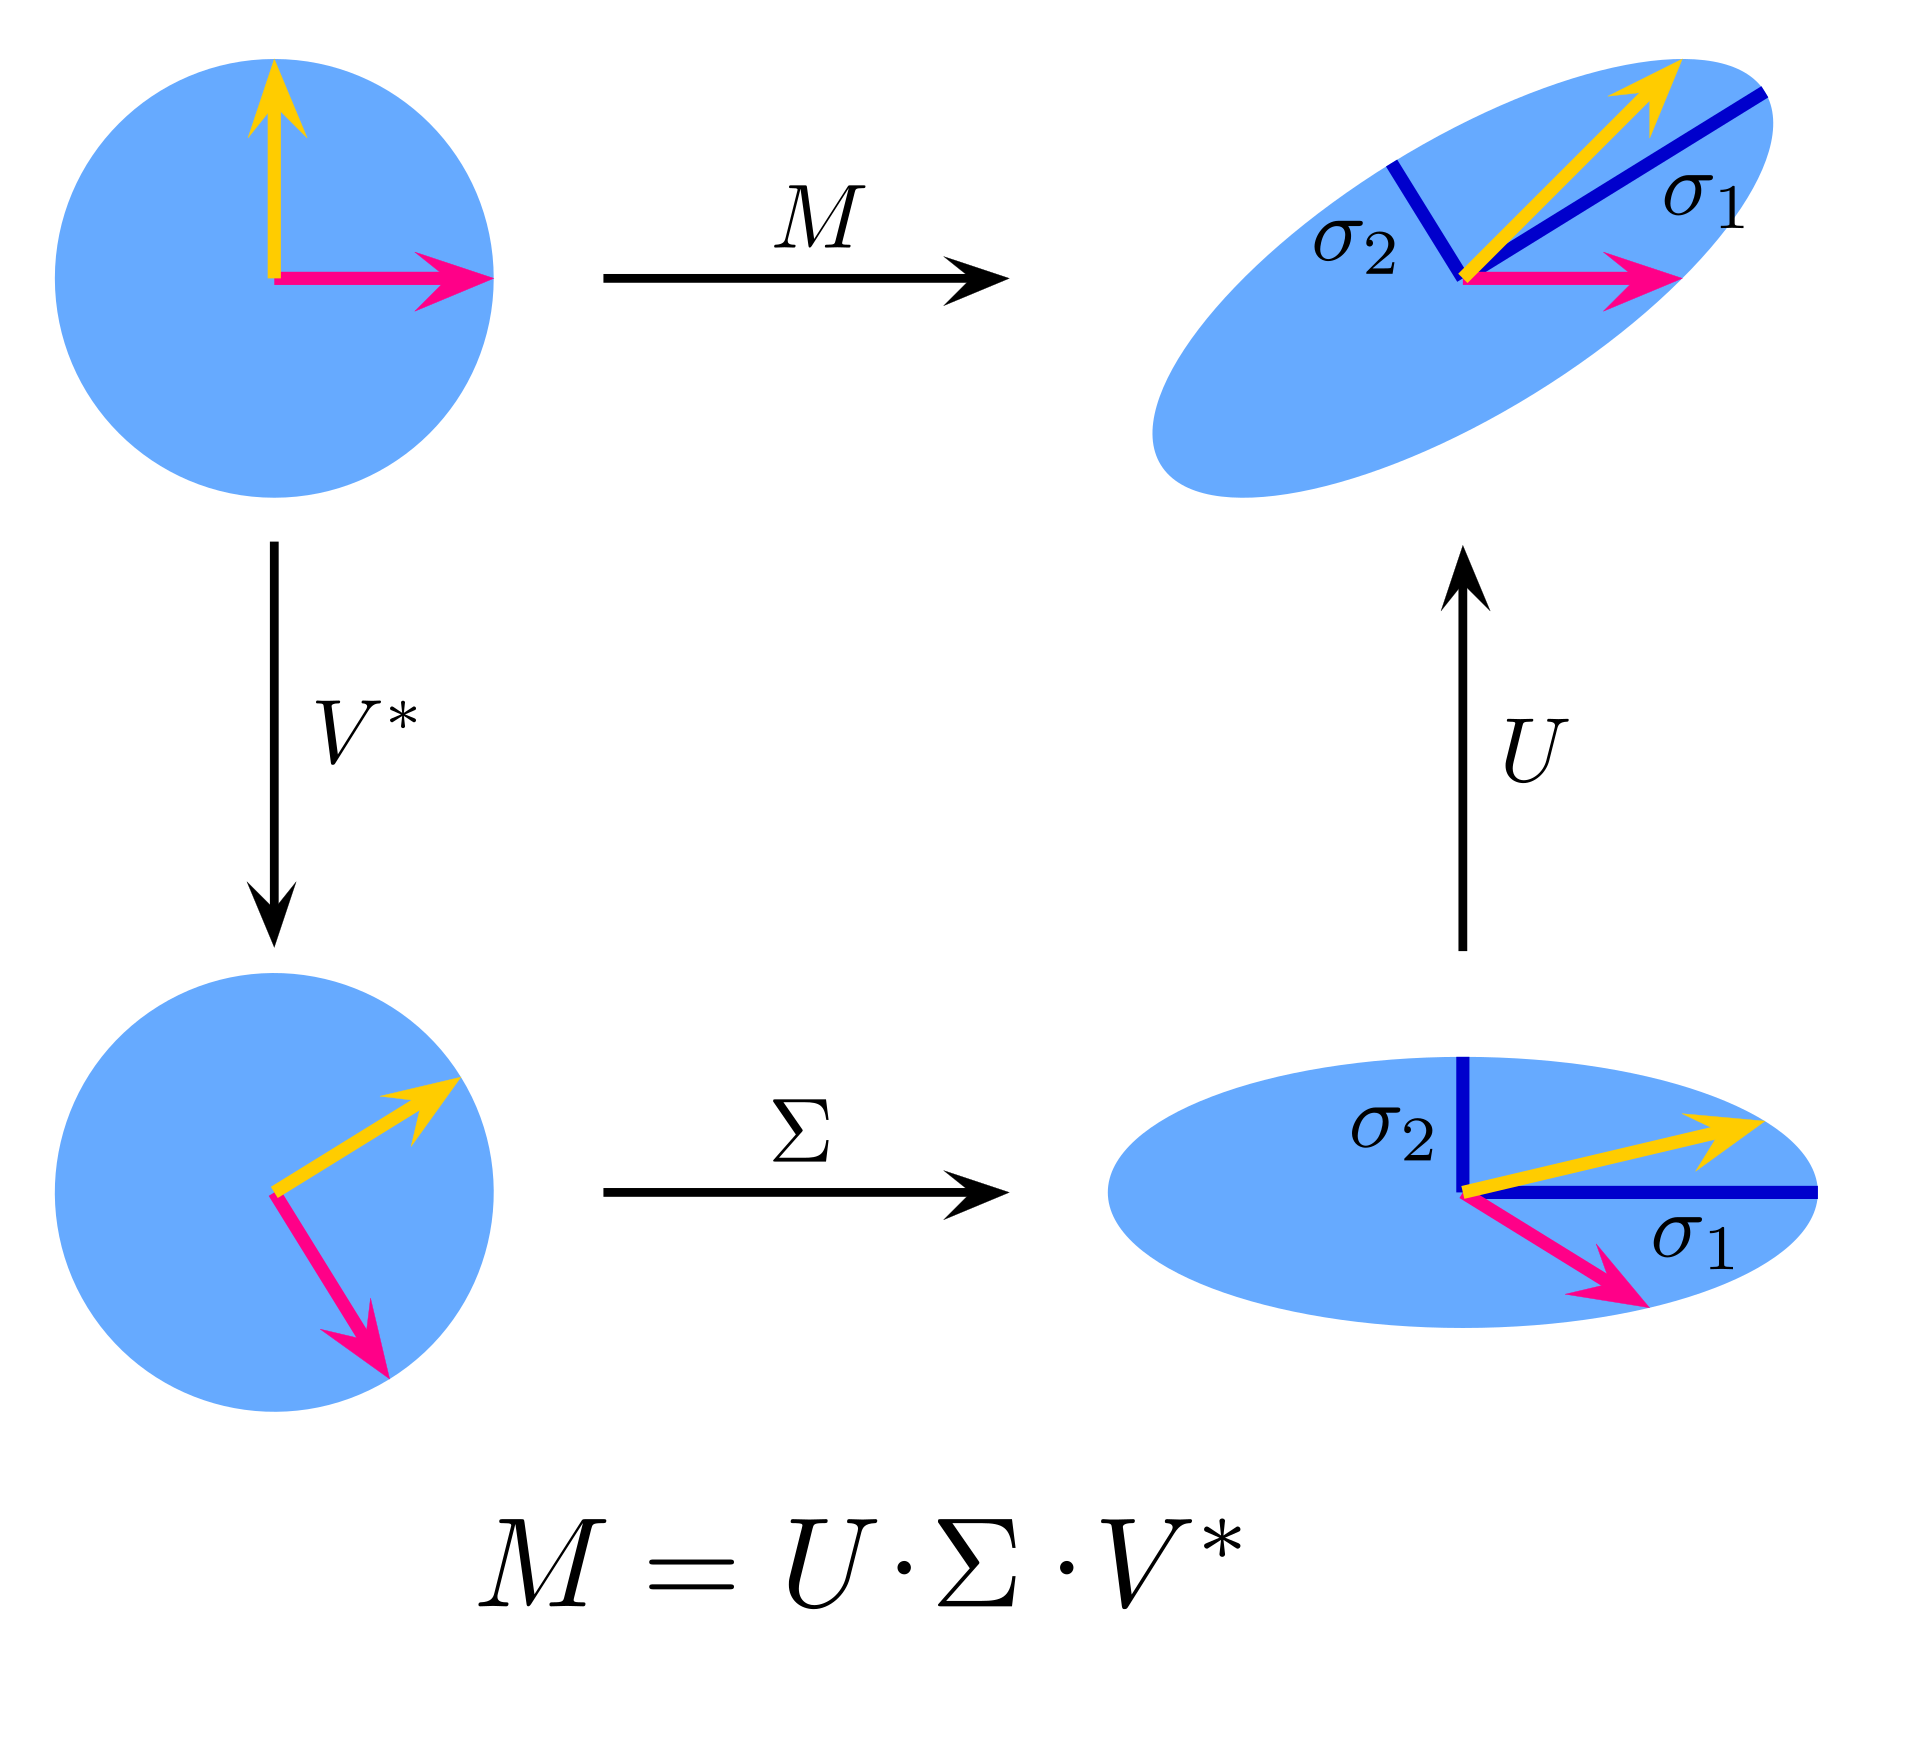
\includegraphics[scale=0.1]{figure/svd.png}
    \caption{Illustration of the singular value decomposition $U\Sigma V^T$ of a real $2\times2$ matrix $M$.
    Down left: The action of $V^T$, is a rotation.
    Down right: The action of $\Sigma$, a scaling by the singular values $\sigma_1$ horizontally and $\sigma_2$ vertically.
    Top right: The action of $U$ is also a rotation.}
    \label{fig:my_label}
\end{figure}

\begin{remark}
The SVD can be thought of as decomposing a matrix into a weighted, ordered sum of separable matrices. By separable, we mean that a matrix A can be written as an outer product of two vectors $X = uv^T$. Specifically, the matrix $A$ can be decomposed as
\begin{equation*}
    A=\sum_{i=1}^n\sigma_i\cdot u_i\cdot v^T_i,
\end{equation*}
where $u_i$ and $v_i$ are the $i$-th columns of the $U,V$, $\sigma_i$ are the ordered singular values. As a result, SVD is widely used in PCA.
\end{remark}

\begin{remark}
For real positive definite symmetric matrix
\begin{itemize}
    \item The columns of $U$ are eigenvectors of $AA^T$.
    \item The columns of $V$ are eigenvectors of $A^TA$.
    \item The non-zero singular values from $\Sigma$ are the square roots of the non-zero eigenvalues of $AA^T$ or $A^TA$.
\end{itemize}
\end{remark}

\begin{remark}
Using the SVD decomposition, we solve $Ax=b$ by
\begin{equation*}
     x=V\Sigma^{-1} U^Tb
\end{equation*}
\end{remark}

\begin{example}
\textbf{SVD in image compression}
The figure below is of the size $450\times 333$, so we can store this image as a matrix $A\in\mathbb{R}^{450\times 333}$. 
\begin{figure}[H]
    \centering
    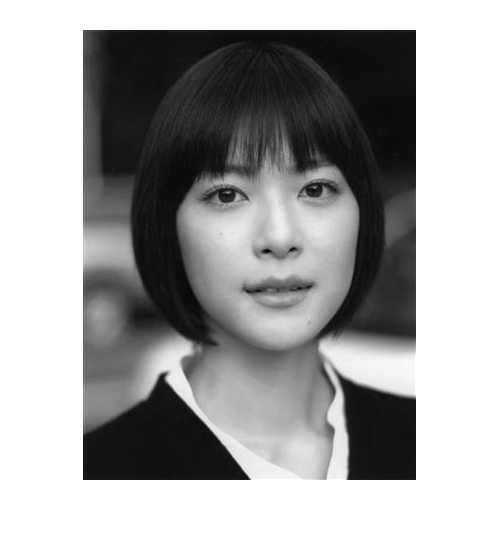
\includegraphics[scale=0.3]{figure/uj_orig.jpg}
    \caption{Original image}
    % \label{fig:my_label}
\end{figure}
Now we can decompose $A$ by SVD as below
\begin{equation*}
    A=\sigma_1u_1v^T_1+\sigma_2u_2v^T_2+\cdots+\sigma_nu_nv^T_n,
\end{equation*}
where $n=\min\{450,333\}$, $u_iv_i^T$ are matrices of rank 1. And assuming $\sigma_1\ge\sigma_2\ge\cdots\ge\sigma_n\ge0$.
And we can see the influence that adding more terms into the image brings in the figure below.
\end{example}
\begin{figure}[H]
    \centering
    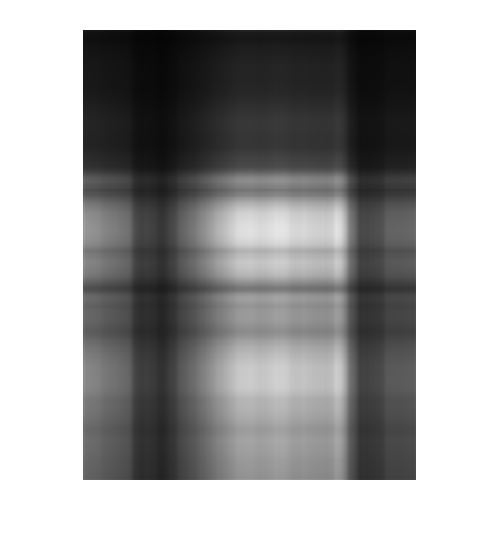
\includegraphics[scale=0.18]{figure/uj_1.png}
    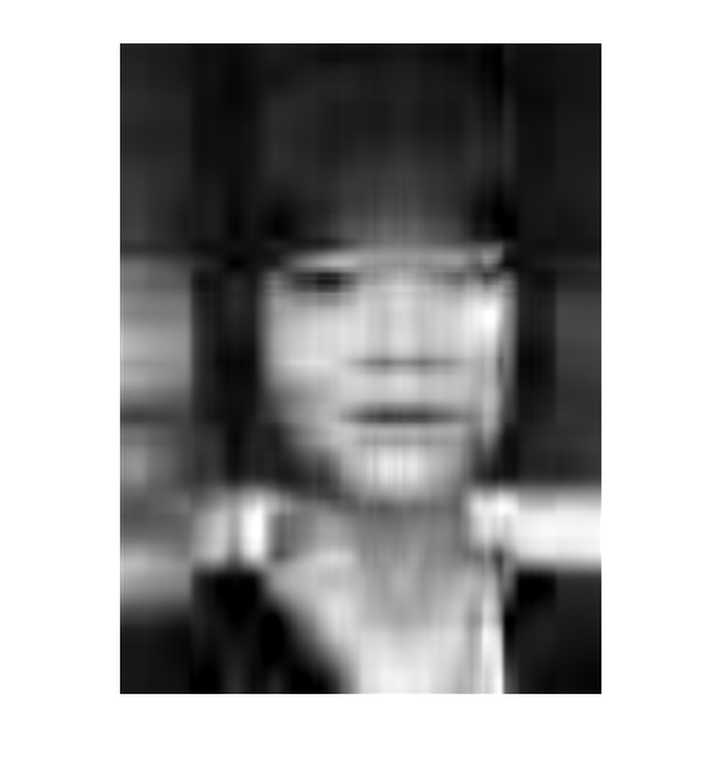
\includegraphics[scale=0.12]{figure/uj_5.jpg}
    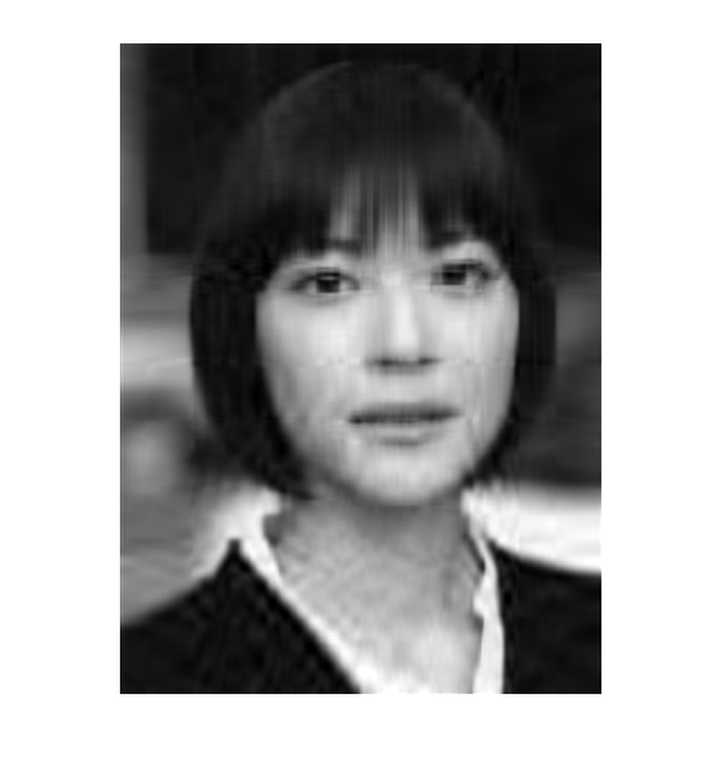
\includegraphics[scale=0.12]{figure/uj_20.jpg}
    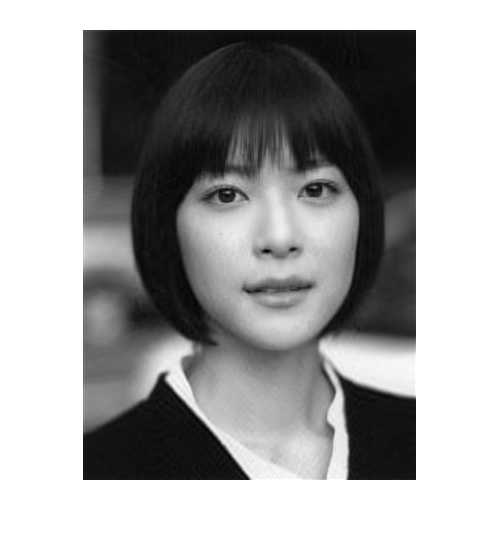
\includegraphics[scale=0.13]{figure/uj_50.jpg}
    \caption{From left to right: only keep the first term; keep the first five terms; keep the first twenty terms; keep the first fifty terms}
    % \label{fig:my_label}
\end{figure}
Without any compression techniques, we need to store $450\times333=149,850$ pixels' value to present an image. With SVD, if we keep the first fifty terms, only $(1+450+333)\times50=39,200$ pixels' value need to be saved, which is 26\% of original size.

\begin{definition}
\boxed{\textbf{Diagonalization.}} Let $A\in\mathbb{R}^{n\times n}$, if there exist invertible matrix $P\in\mathbb{R}^{n\times n}$ such that 
\begin{equation*}
    P^{-1}AP=Diag,
\end{equation*}
then $A$ is diagonalizable.
\end{definition}

\newpage
\section{Geometric Transformations}
\begin{table}[H]
\centering
\begin{tabular}{cccc}
\hline
\textbf{Transformation} & \multicolumn{1}{c}{\textbf{Matrix}} & \textbf{\#DoF} & \textbf{Preserves} \\ \hline
Translation             & $\begin{pmatrix} 1 & 0 & t_1\\ 0 & 1 & t_2\\ 0 & 0 & 1\end{pmatrix}$ & 2              & orientation        \\
Scaling                 & $\begin{pmatrix} s_{1} & 0 & 0\\ 0 & s_{2} & 0\\ 0 & 0 & 1\end{pmatrix}$  & 2 & orientation\\
Shearing                 & $\begin{pmatrix} 1 & s_{1} & 0\\ s_{2} & 1 & 0\\ 0 & 0 & 1\end{pmatrix}$  & 2 & orientation\\
Rotation       & $\begin{pmatrix} \cos(\theta) & -\sin(\theta) & 0\\ \sin(\theta) & \cos(\theta) & 0\\ 0 & 0 & 1\end{pmatrix}$ & 1              & lengths            \\
Affine                  & $\begin{pmatrix} a_{11} & a_{12} & a_{13}\\ a_{21} & a_{22} & a_{23}\\ 0 & 0 & 1\end{pmatrix}$ & 6              & parallelism        \\\hline
\end{tabular}
\end{table}
\begin{remark}
The transformations can be combined by matrix multiplication, of which the order matters,
\begin{align*}
    &\begin{pmatrix} 
        1 & 0 & t_1\\ 
        0 & 1 & t_2\\ 
        0 & 0 & 1
    \end{pmatrix}\cdot
    \begin{pmatrix} 
        \cos(\theta) & -\sin(\theta) & 0\\ 
        \sin(\theta) & \cos(\theta) & 0\\ 
        0 & 0 & 1
    \end{pmatrix}\cdot
    \begin{pmatrix} 
        s_{1} & 0 & 0\\ 
        0 & s_{2} & 0\\ 
        0 & 0 & 1
    \end{pmatrix}\\
    =&\begin{pmatrix} 
        \cos(\theta) & -\sin(\theta) & t_1\\ 
        \sin(\theta) & \cos(\theta) & t_2\\ 
        0 & 0 & 1
    \end{pmatrix}\cdot
    \begin{pmatrix} 
        s_{1} & 0 & 0\\ 
        0 & s_{2} & 0\\ 
        0 & 0 & 1
    \end{pmatrix}\\
    =&\begin{pmatrix} 
        s_1\cos(\theta) & -\sin(\theta) & t_1\\ 
        \sin(\theta) & s_2\cos(\theta) & t_2\\ 
        0 & 0 & 1
    \end{pmatrix}
\end{align*}

especially when there is a translation operation.
\begin{align*}
    &
    \begin{pmatrix} 
        \cos(\theta) & -\sin(\theta) & 0\\ 
        \sin(\theta) & \cos(\theta) & 0\\ 
        0 & 0 & 1
    \end{pmatrix}\cdot
    \begin{pmatrix} 
        s_{1} & 0 & 0\\ 
        0 & s_{2} & 0\\ 
        0 & 0 & 1
    \end{pmatrix}\cdot
    \begin{pmatrix} 
        1 & 0 & t_1\\ 
        0 & 1 & t_2\\ 
        0 & 0 & 1
    \end{pmatrix}\\
    =&\begin{pmatrix} 
        s_1\cos(\theta) & -\sin(\theta) & 0\\ 
        \sin(\theta) & s_2\cos(\theta) & 0\\ 
        0 & 0 & 1
    \end{pmatrix}\cdot
    \begin{pmatrix} 
        1 & 0 & t_1\\ 
        0 & 1 & t_2\\ 
        0 & 0 & 1
    \end{pmatrix}\\
    =&\begin{pmatrix} 
        s_1\cos(\theta) & -\sin(\theta) & s_1t_1\cos(\theta)-t_2\sin(\theta)\\ 
        \sin(\theta) & s_2\cos(\theta) & t_1\sin(\theta)+s_2t_2\cos(\theta)\\ 
        0 & 0 & 1
    \end{pmatrix}
\end{align*}
\end{remark}

\begin{definition}
\boxed{\textbf{Affine transformation}} is a geometric transformation of a Euclidean space that preserves lines and parallelism (but not necessarily distances and angles).
\end{definition}

\begin{remark}
Affine transformations include scaling, rotation, translation, shear mapping, reflection, or compositions of them in any combination and sequence.
\end{remark}

\begin{definition}
\boxed{\textbf{Rigid transformation}} is a geometric transformation of a Euclidean space that preserves the Euclidean distance between every pair of points.
\end{definition}

\begin{remark}
Rigid transformations include rotation, translation, reflection, or compositions of them in any combination and sequence.
\end{remark}
% \begin{table}[H]
% \centering
% \begin{tabular}{ccc}
% \hline
% \multicolumn{1}{l}{\textbf{Transformation}} & { \textbf{Affine}}                  & { \textbf{Rigid}}                   \\ \hline
% Scaling                                     & \cmark & \xmark \\
% Rotation                                    & \cmark & \cmark \\
% Translation                                 & \cmark & \cmark \\
% Shear mapping                               & \cmark & \xmark \\
% Reflection                                  & \cmark & \cmark \\ \hline
% \end{tabular}
% \end{table}
\newpage
\section{Diffusion Tensor Image}
\begin{definition}
\boxed{\textbf{Fractional anisotropy (FA)}} is a scalar value between 0 and 1 that describes the degree of anisotropy of a diffusion process, which is defined as below:
\begin{equation*}
    {\text{FA}}={\sqrt  {{\frac  {3}{2}}}}{\frac  {{\sqrt  {(\lambda _{1}-{\hat  {\lambda }})^{2}+(\lambda _{2}-{\hat  {\lambda }})^{2}+(\lambda _{3}-{\hat  {\lambda }})^{2}}}}{{\sqrt  {\lambda _{1}^{2}+\lambda _{2}^{2}+\lambda _{3}^{2}}}}}
\end{equation*}
where
\begin{equation*}
     {\hat {\lambda }}=(\lambda _{1}+\lambda _{2}+\lambda _{3})/3.
\end{equation*}
\end{definition}

\begin{remark}
When $\operatorname{FA}=0$, the tensor is a sphere. The FA more close to 1, the tensor more anisotropy.
\end{remark}

\begin{definition}
\boxed{\textbf{DWI signal}} $S_j$ in a voxel $x$ is defined as below:
\begin{equation*}
    S_j(x)=S_0(x)e^{-bg^T_jD(x)g_j}
\end{equation*}
where $b$ is the know b-value, $S_0$ is the acquired baseline image, $D(x)$ is the diffusion tensor at voxel $x$, and $g_j$ is the $j$-th gradient encoding direction.
\end{definition}

\begin{definition}
\boxed{\textbf{Deterministic tractography}} computes streamlines (sometimes called fibers) by forward integration of the principal eigenvector of the diffusion tensors from one region.
\end{definition}

\begin{remark}
One major problem with tractography is that imaging noise causes errors in the principal eigenvector direction, and these errors accumulate in the integration of the streamlines. Another disadvantage to tractography is that it has difficulty in cases where the goal is to find pathways between two regions.
\end{remark}

\begin{remark}
Tractography is simply the Euler integration on the principal eigenvector field(red vector in figure below) derived by DTI image, while the geodesic will follow the tangent vector(blue vector in figure below). And that's the reason why the geodesic will deviate from the integral curve among the high curvature area. Principal eigenvector of the metric tensor and tangent vector of the metric tensor are not necessarily the same.
\end{remark}

\begin{figure}[H]
    \centering
    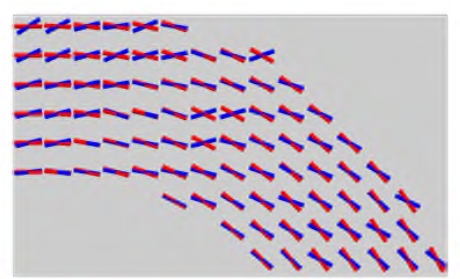
\includegraphics[scale=0.5]{figure/teneigen.png}
    \caption{Tangent vectors of the geodesics (blue) of the generated noisy data at a SNR of 15 under the inverse-tensor metric without modulation. The red vectors are the principal eigenvectors of the diffusion tensors.}
    % \label{fig:my_label}
\end{figure}

\newpage
\section{Deep Learning}
\subsection{Common terms}
\begin{definition}
One \boxed{\textbf{batch}} of samples is a group of samples concatenated together to go through the network before updating the model weights.
\end{definition}

\begin{table}[H]
\centering
\begin{tabular}{cc}
\hline
{ \textbf{Types}}              & { \textbf{Batch size}}                    \\ \hline
Stochastic gradient descent & 1 \\
Mini-Batch gradient descent & $(1, \text{size of training dataset})$\\
Batch gradient descent      & size of training dataset \\ \hline
\end{tabular}
\end{table}

\begin{example}
In PyTorch's implementation, mini-batch concatenates the designated samples together and put it into the network. For instance, if the image is of size 128*128*128, 4 channels, and mini-batch size is 2, then the shape of input tensor during training is 2*4*128*128*128. 

You may wonder that when it comes to testing, the input is only one sample at a time, but the model stays the same, how can that still work? The things is, a model only regulates the shape of convolution kernel, pooling parameters, activation function and how they are organized, the size of the input does not matter, it can either 2*4*128*128*128 or 1*4*128*128*128. The final loss is actually summation of all samples' loss. As long as the output size matches the ground-truth size, the workflow can be performed uninterruptedly.
\end{example}

\begin{definition}
One \boxed{\textbf{iteration}} is a time span when an a batch of training data is passed forward and backward through the neural network.
\end{definition}

\begin{definition}
One \boxed{\textbf{epoch}} is a time span when an entire training dataset is passed forward and backward through the neural network.
\end{definition}

\subsection{Loss Functions}
\begin{definition}
\boxed{\textbf{Intersection of Union(Jaccard index, IoU)}} is defined as 
\begin{equation*}
    \operatorname{IoU}=\frac{|A\cap B|}{|A\cup B|}
\end{equation*}
\end{definition}

\begin{definition}
\boxed{\textbf{Dice loss function}} is defined as 
\begin{equation*}
    L_{\operatorname{dice}}=-\frac{2|A\cap B|}{|A|+|B|}=-\frac{2\times\left<v_{\operatorname{true}}, v_{\operatorname{pred}}\right>}{\|v_{\operatorname{true}}\|^2_2+\|v_{\operatorname{pred}}\|^2_2+\epsilon}\in(-1,0],
\end{equation*}
where $v_{\operatorname{true}},v_{\operatorname{pred}}\in\mathbb{R}^{h\times w\times d}$ are \textbf{one-hot vectors}, and $\epsilon$ is a small constant to avoid zero division. 
\end{definition}

\begin{remark}
Since dice loss function is a loss function, just as other loss function, lower score indicates better alignment. And that's the reason why the negative sign is indispensable.
\end{remark}

\begin{definition}
\boxed{\textbf{$L^1$ loss function}} is defined as 
\begin{equation*}
    L_{L^1}=\|v_{\operatorname{true}}-v_{\operatorname{pred}}\|_1,
\end{equation*}
where $v_{\operatorname{true}},v_{\operatorname{pred}}$ are vectors.
\end{definition}

\begin{definition}
\boxed{\textbf{$L^2$ loss function}} is defined as 
\begin{equation*}
    L_{L^2}=\|v_{\operatorname{true}}-v_{\operatorname{pred}}\|^2_2,
\end{equation*}
where $v_{\operatorname{true}},v_{\operatorname{pred}}$ are vectors.
\end{definition}

\begin{definition}
\boxed{\textbf{Hausdorff distance}} is defined as 
\begin{equation*}
     d_{\mathrm {H} }(X,Y)=\max \left\{\,\sup _{x\in X}\inf _{y\in Y}d(x,y),\,\sup _{y\in Y}\inf _{x\in X}d(x,y)\,\right\}
\end{equation*}
where X and Y be two non-empty subsets of a metric space $(M,d)$.
\end{definition}

\begin{figure}[H]
    \centering
    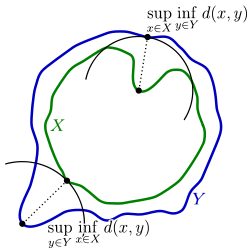
\includegraphics[scale=0.6]{figure/hausdorff.png}
    \caption{Components of the calculation of the Hausdorff distance between the green line X and the blue line Y.}
\end{figure}

\begin{definition}
\boxed{\textbf{Entropy}} of the \textbf{discrete probability distribution} $p$ is defined as
\begin{equation*}
   H(p)=-\sum _{x\in {\mathcal {X}}}{p (x)\log p (x)} \in[0,1]
\end{equation*}

\begin{remark}
If entropy is closer to 1, means the distribution is of high level of disorder (low level of purity). If entropy is closer to 0, means the distribution is of low level of disorder (high level of purity).
\end{remark}

\begin{definition}
\boxed{\textbf{Cross-entropy loss function}} of the \textbf{discrete probability distribution} $p$ and $q$ over a given set is defined as 
\begin{equation*}
    H(p,q)=-\sum_{x\in {\mathcal {X}}} p(x)\log(q(x))=-\left<p,\log(q)\right>\in[0,\infty),
\end{equation*}
which measures the distance between the distributions.
\end{definition}

\begin{remark}
Cross-entropy loss, or log loss, measures the performance of a classification model whose output is a \textbf{probability value between 0 and 1}. Cross-entropy loss increases as the predicted probability diverges from the actual label. 
\end{remark}

\end{definition}

\begin{example}
As for the two discrete distributions below:
\begin{table}[H]
\centering
\begin{tabular}{cccc}
\hline
\textbf{Distribution} & \textbf{Class A} & \textbf{Class B} & \textbf{Class C} \\ \hline
$p$            & 0       & 0       & 1    \\ 
$q$           & 0.1     & 0.2     & 0.7        \\ \hline
\end{tabular}
\end{table}
we can have the cross entropy 
\begin{equation*}
    H(p,q)=-(0\times\log(0.1)+0\times\log(0.2)+0\times\log(0.7))=0.35
\end{equation*}
\end{example}

\begin{remark}
According to the example above, the only thing that contributes to the value of loss is the predicted possibility of the ground-truth class, since the possibilities of other classes are all wiped out by 0. The closer predicted possibility of the ground-truth class to 1, the lower loss will be.
\begin{figure}[H]
    \centering
    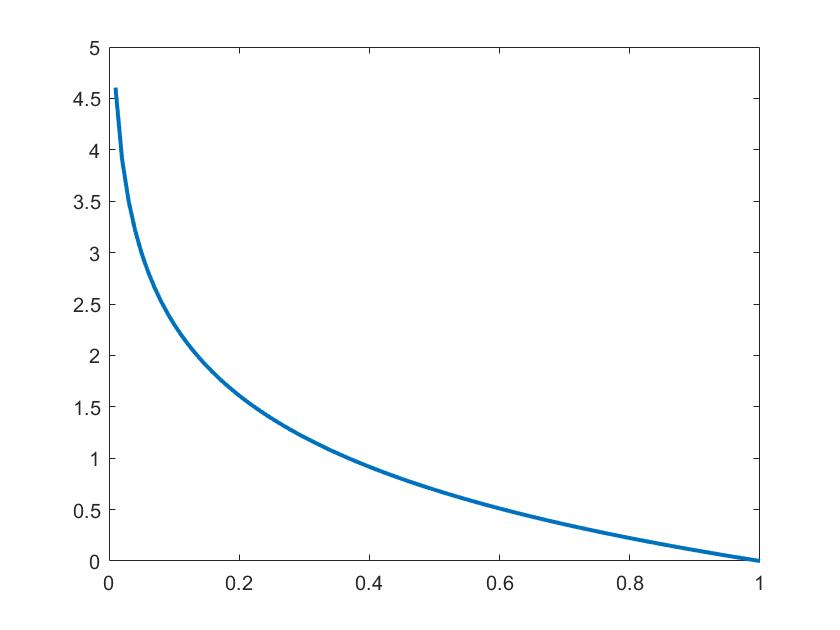
\includegraphics[scale=0.25]{figure/log.jpg}
    \caption{$y=-\log(x)$}
    \label{fig:my_label}
\end{figure}
\end{remark}

\begin{definition}
\boxed{\textbf{Kullback–Leibler(KL) divergence}} is defined as
\begin{align*}
    D_{\text{KL}}(p,q)&=\sum _{x\in {\mathcal {X}}}p(x)\log \left({\frac {p(x)}{q(x)}}\right)\\
    &=-\sum _{x\in {\mathcal {X}}}p(x)\log q(x)+\sum _{x\in {\mathcal {X}}}p(x)\log p(x)\\
    &=-H(p,q)+H(p)\in[0,\infty),
\end{align*}
\end{definition}

\begin{remark}
KL divergence describes how different $q$ is from $p$ from the perspective of $p$. When $p$ is fixed, just as the ground-truth data in training, minimizing KL divergence and cross-entropy is equivalent, as $H(p)$ is a constant.
\end{remark}

\begin{example}
As for the two discrete distributions below:
\begin{table}[H]
\centering
\begin{tabular}{cccc}
\hline
\textbf{Distribution} & \textbf{Class A} & \textbf{Class B} & \textbf{Class C} \\ \hline
$p$            & 0       & 0       & 1    \\ 
$q$           & 0.1     & 0.2     & 0.7        \\ \hline
\end{tabular}
\end{table}
we can have the KL divergence
\begin{equation*}
    D_{\operatorname{KL}}(p,q)=(0\times\log(0)+0\times\log(0)+1\times\log(1))-(0\times\log(0.1)+0\times\log(0.2)+0\times\log(0.7))=0.35
\end{equation*}
\end{example}

\subsection{Normalization}
\begin{definition}
\boxed{\textbf{Batch normalization}}\cite{batch} is defined as
\begin{align*}
     \mu_{c}&=\frac{1}{HWN}\sum^N_n\sum^W_w\sum^H_h x_{cnhw}\\
     \sigma_{c}^2&=\frac{1}{HWN}\sum^N_n\sum^W_w\sum^H_h(x_{cnhw}-\mu_c)^2\\
     \hat{x}_{c}&=\frac{x_{c}-\mu_{c}}{\sqrt{\sigma_{c}^2+\epsilon}}
\end{align*}
where $x$ are the values of input over a mini-batch, $C,N,H,W$ are the channel, batch, height, width size, respectively. Batch normalization should be performed by each channel.
\end{definition}

\begin{definition}
\boxed{\textbf{Layer normalization}} is defined as
\begin{align*}
     \mu_{n}&=\frac{1}{HWC}\sum^C_c\sum^W_w\sum^H_h x_{cnhw}\\
     \sigma_{n}^2&=\frac{1}{HWC}\sum^C_c\sum^W_w\sum^H_h(x_{cnhw}-\mu_n)^2\\
     \hat{x}_{n}&=\frac{x_{n}-\mu_{n}}{\sqrt{\sigma_{n}^2+\epsilon}}
\end{align*}
where $x$ are the values of input over a mini-batch, $C,N,H,W$ are the channel, batch, height, width size, respectively. Layer normalization should be performed by each sample in a mini-batch.
\end{definition}

\begin{definition}
\boxed{\textbf{Instance normalization}} is defined as
\begin{align*}
     \mu_{cn}&=\frac{1}{HW}\sum^W_w\sum^H_h x_{cnhw}\\
     \sigma_{cn}^2&=\frac{1}{HW}\sum^W_w\sum^H_h(x_{cnhw}-\mu_{cn})^2\\
     \hat{x}_{cn}&=\frac{x_{cn}-\mu_{cn}}{\sqrt{\sigma_{cn}^2+\epsilon}}
\end{align*}
where $x$ are the values of input over a mini-batch, $C,N,H,W$ are the channel, batch, height, width size, respectively. Instance normalization should be performed by each channel and sample in a batch.
\end{definition}

\begin{definition}
\boxed{\textbf{Group normalization}}\cite{group} is a middle ground between layer and instance normalization, which is defined as
\begin{align*}
     \mu_{gn}&=\frac{1}{HW|G_i|}\sum^{|G_i|}_{c\in G_i}\sum^W_w\sum^H_h x_{cnhw}\\
     \sigma_{gn}^2&=\frac{1}{HW|G_i|}\sum^{|G_i|}_{c\in G_i}\sum^W_w\sum^H_h(x_{cnhw}-\mu_n)^2\\
     \hat{x}_{gn}&=\frac{x_{n}-\mu_{n}}{\sqrt{\sigma_{n}^2+\epsilon}}\\
     G&=\{G_1,\cdots\}\\
     G_i&=\{c_i,\cdots,c_{i'}\}
\end{align*}
where $x$ are the values of input over a mini-batch, $C,N,H,W,|G|$ are the channel, batch, height, width, group size, respectively. Instance normalization should be performed by each group among the channel set.
\end{definition}

\begin{figure}[H]
    \centering
    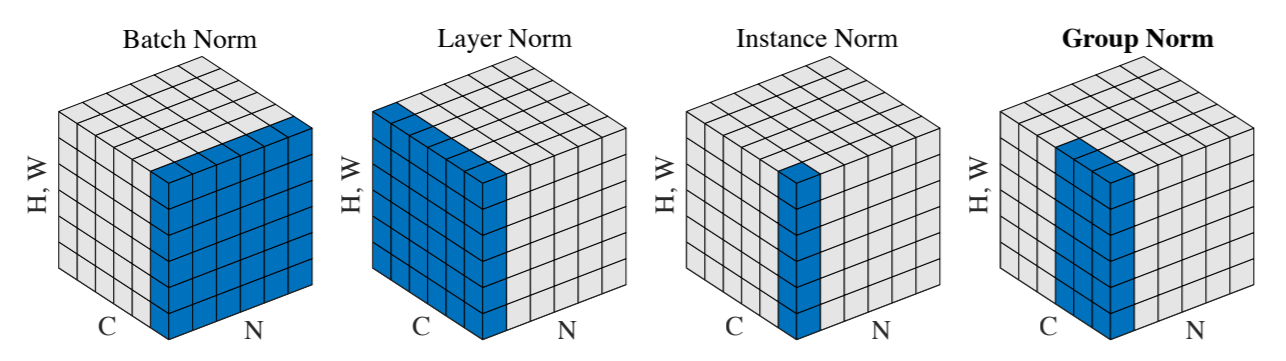
\includegraphics[scale=0.4]{figure/normalization.png}
    \caption{Normalization methods. Each subplot shows a feature map tensor, with $N$ as the batch axis, $C$ as the channel axis, and $(H, W)$ as the spatial axes. The pixels in blue are normalized by the same mean and variance, computed by aggregating the values of these pixels.}
    \label{fig:my_label}
\end{figure}

\subsection{Optimizer}
\begin{definition}
\boxed{\textbf{Adam optimizer}}
\end{definition}
\subsection{Regularization}
\subsection{Activation Function}
\begin{table}[H]
\centering
\begin{tabular}{cccc}
\hline
\textbf{Types}                    & \textbf{Functions}                                       & \textbf{Range}                                           & \textbf{Order of continuity} \\ \hline
Sigmoid(logistic)        & $\sigma(x)=\frac {1}{1+e^{-x}}$               & $(0,1)$  & $C^\infty$\\
Tanh(hyperbolic tangent) & $\tanh(x)={\frac {e^{x}-e^{-x}}{e^{x}+e^{-x}}}$ & $(-1,1)$   & $C^\infty$\\
ReLU(rectified linear unit)  & $\operatorname{ReLU}(x)=\max\{0,x\}$            & $[0,+\infty)$    & $C^0$\\       
Leaky ReLU               & $\operatorname{Leaky ReLU}(x)=\max\{0.01x,x\}$  & $(-\infty,+\infty)$ & $C^0$\\
ELU(exponential linear unit)& ${\begin{cases}\alpha \left(e^{x}-1\right)&{\text{if }}x\leq 0\\x&{\text{if }}x>0\end{cases}}$ & $(-\alpha,+\infty)$ & $\begin{cases}C^{1}&{\text{if }}\alpha =1\\C^{0}&{\text{otherwise}}\end{cases}$\\ 
GELU(gaussian error linear unit)& $\begin{aligned}&{\frac {1}{2}}x\left(1+{\text{erf}}\left({\frac {x}{\sqrt {2}}}\right)\right)\end{aligned}$ & $(-0.17,+\infty)$ & $C^\infty$\\
\hline
\end{tabular}
\end{table}

\begin{figure}[H]
    \centering
    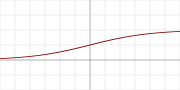
\includegraphics[scale=0.6]{figure/sigmoid.png}
    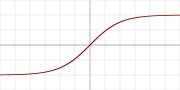
\includegraphics[scale=0.6]{figure/tanh.png}
    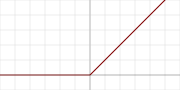
\includegraphics[scale=0.6]{figure/relu.png}
    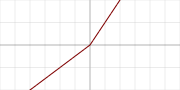
\includegraphics[scale=0.6]{figure/leakyrelu.png}
    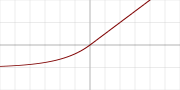
\includegraphics[scale=0.6]{figure/elu.png}
    \includegraphics[scale=0.08]{figure/gelu.png}
    \caption{Plots of sigmoid, tahn, ReLU, Leaky ReLU, ELU, GELU activation functions, correspondingly.}
\end{figure}

The following table lists activation functions that are not functions of a single fold $x$ from the previous layer or layers:
\begin{table}[H]
\centering
\begin{tabular}{cccc}
\hline
{ \textbf{Types}} & { \textbf{Functions}}                            & { \textbf{Range}}        & { \textbf{Order of continuity}} \\ \hline
{ Softmax}        & { $\frac {e^{x_{i}}}{\sum _{j=1}^{J}e^{x_{j}}}$} & { $(0,1)$}               & { $C^{\infty }$}                \\ 
{ Maxout}         & { $\max _{i}x_{i}$}                              & { $ (-\infty ,\infty )$} & { $C^{0}$}                      \\ \hline
\end{tabular}
\end{table}

\begin{remark}
Activation functions have different mathematical properties:
\begin{itemize}
    \item \textbf{Nonlinear.} When the activation function is non-linear, then a two-layer neural network can be proven to be a universal function approximator. This is known as the Universal Approximation Theorem. The identity activation function does not satisfy this property. When multiple layers use the identity activation function, the entire network is equivalent to a single-layer model.
    \item \textbf{Range.} When the range of the activation function is finite, gradient-based training methods tend to be more stable, because pattern presentations significantly affect only limited weights. When the range is infinite, training is generally more efficient because pattern presentations significantly affect most of the weights. In the latter case, smaller learning rates are typically necessary.
    \item \textbf{Continuously differentiable.} This property is desirable (ReLU is not continuously differentiable and has some issues with gradient-based optimization, but it is still possible) for enabling gradient-based optimization methods. The binary step activation function is not differentiable at 0, and it differentiates to 0 for all other values, so gradient-based methods can make no progress with it.
    \item \textbf{Monotonic.} When the activation function is monotonic, the error surface associated with a single-layer model is guaranteed to be convex.
\end{itemize}
\end{remark}
\subsection{Data Augmentation}

\newpage
\begin{thebibliography}{99} 
\bibitem{optimization}Luenberger, D.G., 1997. \textit{Optimization by vector space methods}. John Wiley \& Sons.
\bibitem{fletcher}Fletcher, P.T., Pizer, S.M. and Joshi, S., 2004. \textit{Statistical variability in nonlinear spaces: Application to shape analysis and DT-MRI} (pp. 6469-6469). University of North Carolina at Chapel Hill.
\bibitem{hao}Hao, X., 2014. \textit{Improved segmentation and analysis of white matter tracts based on adaptive geodesic tracking}. The University of Utah.
\bibitem{zhang}Zhang, M., 2016. \textit{Bayesian models on manifolds for image registration and statistical shape analysis}. The University of Utah.
\bibitem{singh}Singh, N.P., 2013. \textit{Multivariate regression of shapes via deformation momenta: Application to quantifying brain atrophy in aging and dementia}. The University of Utah.
\bibitem{yger}Yger, F., Berar, M. and Lotte, F., 2016. \textit{Riemannian approaches in brain-computer interfaces: a review}. IEEE Transactions on Neural Systems and Rehabilitation Engineering, 25(10), pp.1753-1762.
\bibitem{bhatia}Bhatia, R., 2009. \textit{Positive definite matrices} (Vol. 24). Princeton university press.
\bibitem{robbin}Robbin, J.W. and Salamon, D.A., 2011. \textit{Introduction to differential geometry}. ETH, Lecture Notes, preliminary version.
\bibitem{stanford} Lecture 4 Note: Surface Theory I. PDF file. Spring, 2013. \url{https://graphics.stanford.edu/courses/cs468-13-spring/assets/lecture4-suteparuk.pdf}
\bibitem{stanford2} Lecture 10: Computing Geodesics. PDF file. Spring, 2013. \url{https://graphics.stanford.edu/courses/cs468-13-spring/assets/lecture10-lukaczyk.pdf}
\bibitem{stanford3} Lecture 15: Isometries, Rigidity and Curvature. PDF file. Spring, 2013. \url{https://graphics.stanford.edu/courses/cs468-13-spring/assets/lecture15-lindsey.pdf}
\bibitem{stanford4} Lecture 19: Conformal Geometry. PDF file. Spring, 2013. \url{https://graphics.stanford.edu/courses/cs468-13-spring/assets/lecture19-buganza-tepole.pdf}
\bibitem{ucl} Introduction to RKHS, and some simple kernel
algorithms. PDF file. October 16, 2019. \url{http://www.gatsby.ucl.ac.uk/~gretton/coursefiles/lecture4_introToRKHS.pdf}
\bibitem{cd1} Tensor Calculus 17: The Covariant Derivative (flat space). YouTube. September 25, 2018. \url{https://www.youtube.com/watch?v=U5iMpOn5IHw&list=LLVT8QysnCZqdisAyo0CI0-g&index=2}
\bibitem{cd2} Tensor Calculus 18: Covariant Derivative (extrinsic) and Parallel Transport. YouTube. October 16, 2018. \url{https://www.youtube.com/watch?v=Af9JUiQtV1k&list=LLVT8QysnCZqdisAyo0CI0-g&index=2&t=1482s}
\bibitem{cd3} Tensor Calculus 19: Covariant Derivative (Intrinsic) and Geodesics. YouTube. October 27, 2018. \url{https://www.youtube.com/watch?v=EFKBp52LtDM&t=146s}
\bibitem{metric} Tensors for Beginners 9: The Metric Tensor. YouTube. January 27, 2018. \url{https://www.youtube.com/watch?v=C76lWSOTqnc}
\bibitem{shift} PROPERTIES OF THE DFT. PDF file. \url{http://eeweb.poly.edu/iselesni/EL713/zoom/dftprop.pdf}
\bibitem{rg} Riemannian Geometry: Definitions, Pictures, and Results. PDF file. \url{https://arxiv.org/pdf/1412.2393.pdf}
\bibitem{karcher} Karcher, H., 1977. Riemannian center of mass and mollifier smoothing. Communications on pure and applied mathematics, 30(5), pp.509-541.
\bibitem{tomthesis}Fletcher, P.T., Statistical Variability in Nonlinear Spaces: Application to Shape Analysis and DT-MRI, Ph.D. Thesis, Department of Computer Science, University of North Carolina, August 2004.
\bibitem{batch}Ioffe, S. and Szegedy, C., 2015, June. Batch normalization: Accelerating deep network training by reducing internal covariate shift. In International conference on machine learning (pp. 448-456). PMLR.
\bibitem{group}Wu, Y. and He, K., 2018. Group normalization. In Proceedings of the European conference on computer vision (ECCV) (pp. 3-19).
\end{thebibliography}
\end{document}